\documentclass[journal=jacsat,manuscript=article]{achemso}

\usepackage[version=3]{mhchem} % Formula subscripts using \ce{}
\usepackage{comment}

\newcommand*\mycommand[1]{\texttt{\emph{#1}}}

\author{Carlo Andrea De Filippo}
\affiliation{Science Department, University of Roma Tre, Via della Vasca Navale 84, 00146, Rome, Italy}
\email{carloandrea.defilippo@uniroma3.it}

\author{Pietro Corsi}
\affiliation{Science Department, University of Roma Tre, Via della Vasca Navale 84, 00146, Rome, Italy}


\author{Cristiano De Michele}
\affiliation{Physics Department, University of Rome ``La Sapienza'', Piazzale Aldo Moro 2, Rome, Italy}

\author{Barbara Capone}
\affiliation{Science Department, University of Roma Tre, Via della Vasca Navale 84, 00146, Rome, Italy}
\email{barbara.capone@uniroma3.it}

\title{Supporting information}
  
 \begin{document}


\section{Initial configuration}

The particles are initially arranged in a orthorhombic lattice with number of particles $\vec{n} = (18, 18, 4)$ and intermolecular distances set as $\vec{a} = 1.1 \, (D_{max}, D_{max}, L_{max} + D_{max})$, where $D_{max}$ and $L_{max}$ are the maximum diameter and length of the particles in the system. 


\begin{figure}[!h]
    \centering
    \includegraphics[width=0.5 \columnwidth]{Figures/Initial_conf.png}
    \caption{Snapshot of the orthorhombic initial configuration for a system of spherocylinders with $A = 5$. A) monodisperse system. B) system with polydispersity on L. C) system with polydispersity on D. (DA MODIFICARE METTENDO LE DIVERSE DISTANZE E NUOVI TIPI DI SIMULAZIONI)}
    \label{fig:Initial_conf}
\end{figure}

%%%%%%%%%%%%%%%%%%%

\section{Complete EOS of the systems for all the elongations}

In fig. \ref{fig:EOS_tot} are represented all the equations of state of the different polydispersities as a function of the average aspect ratio of the particles.

\begin{figure}[!h]
    \centering
    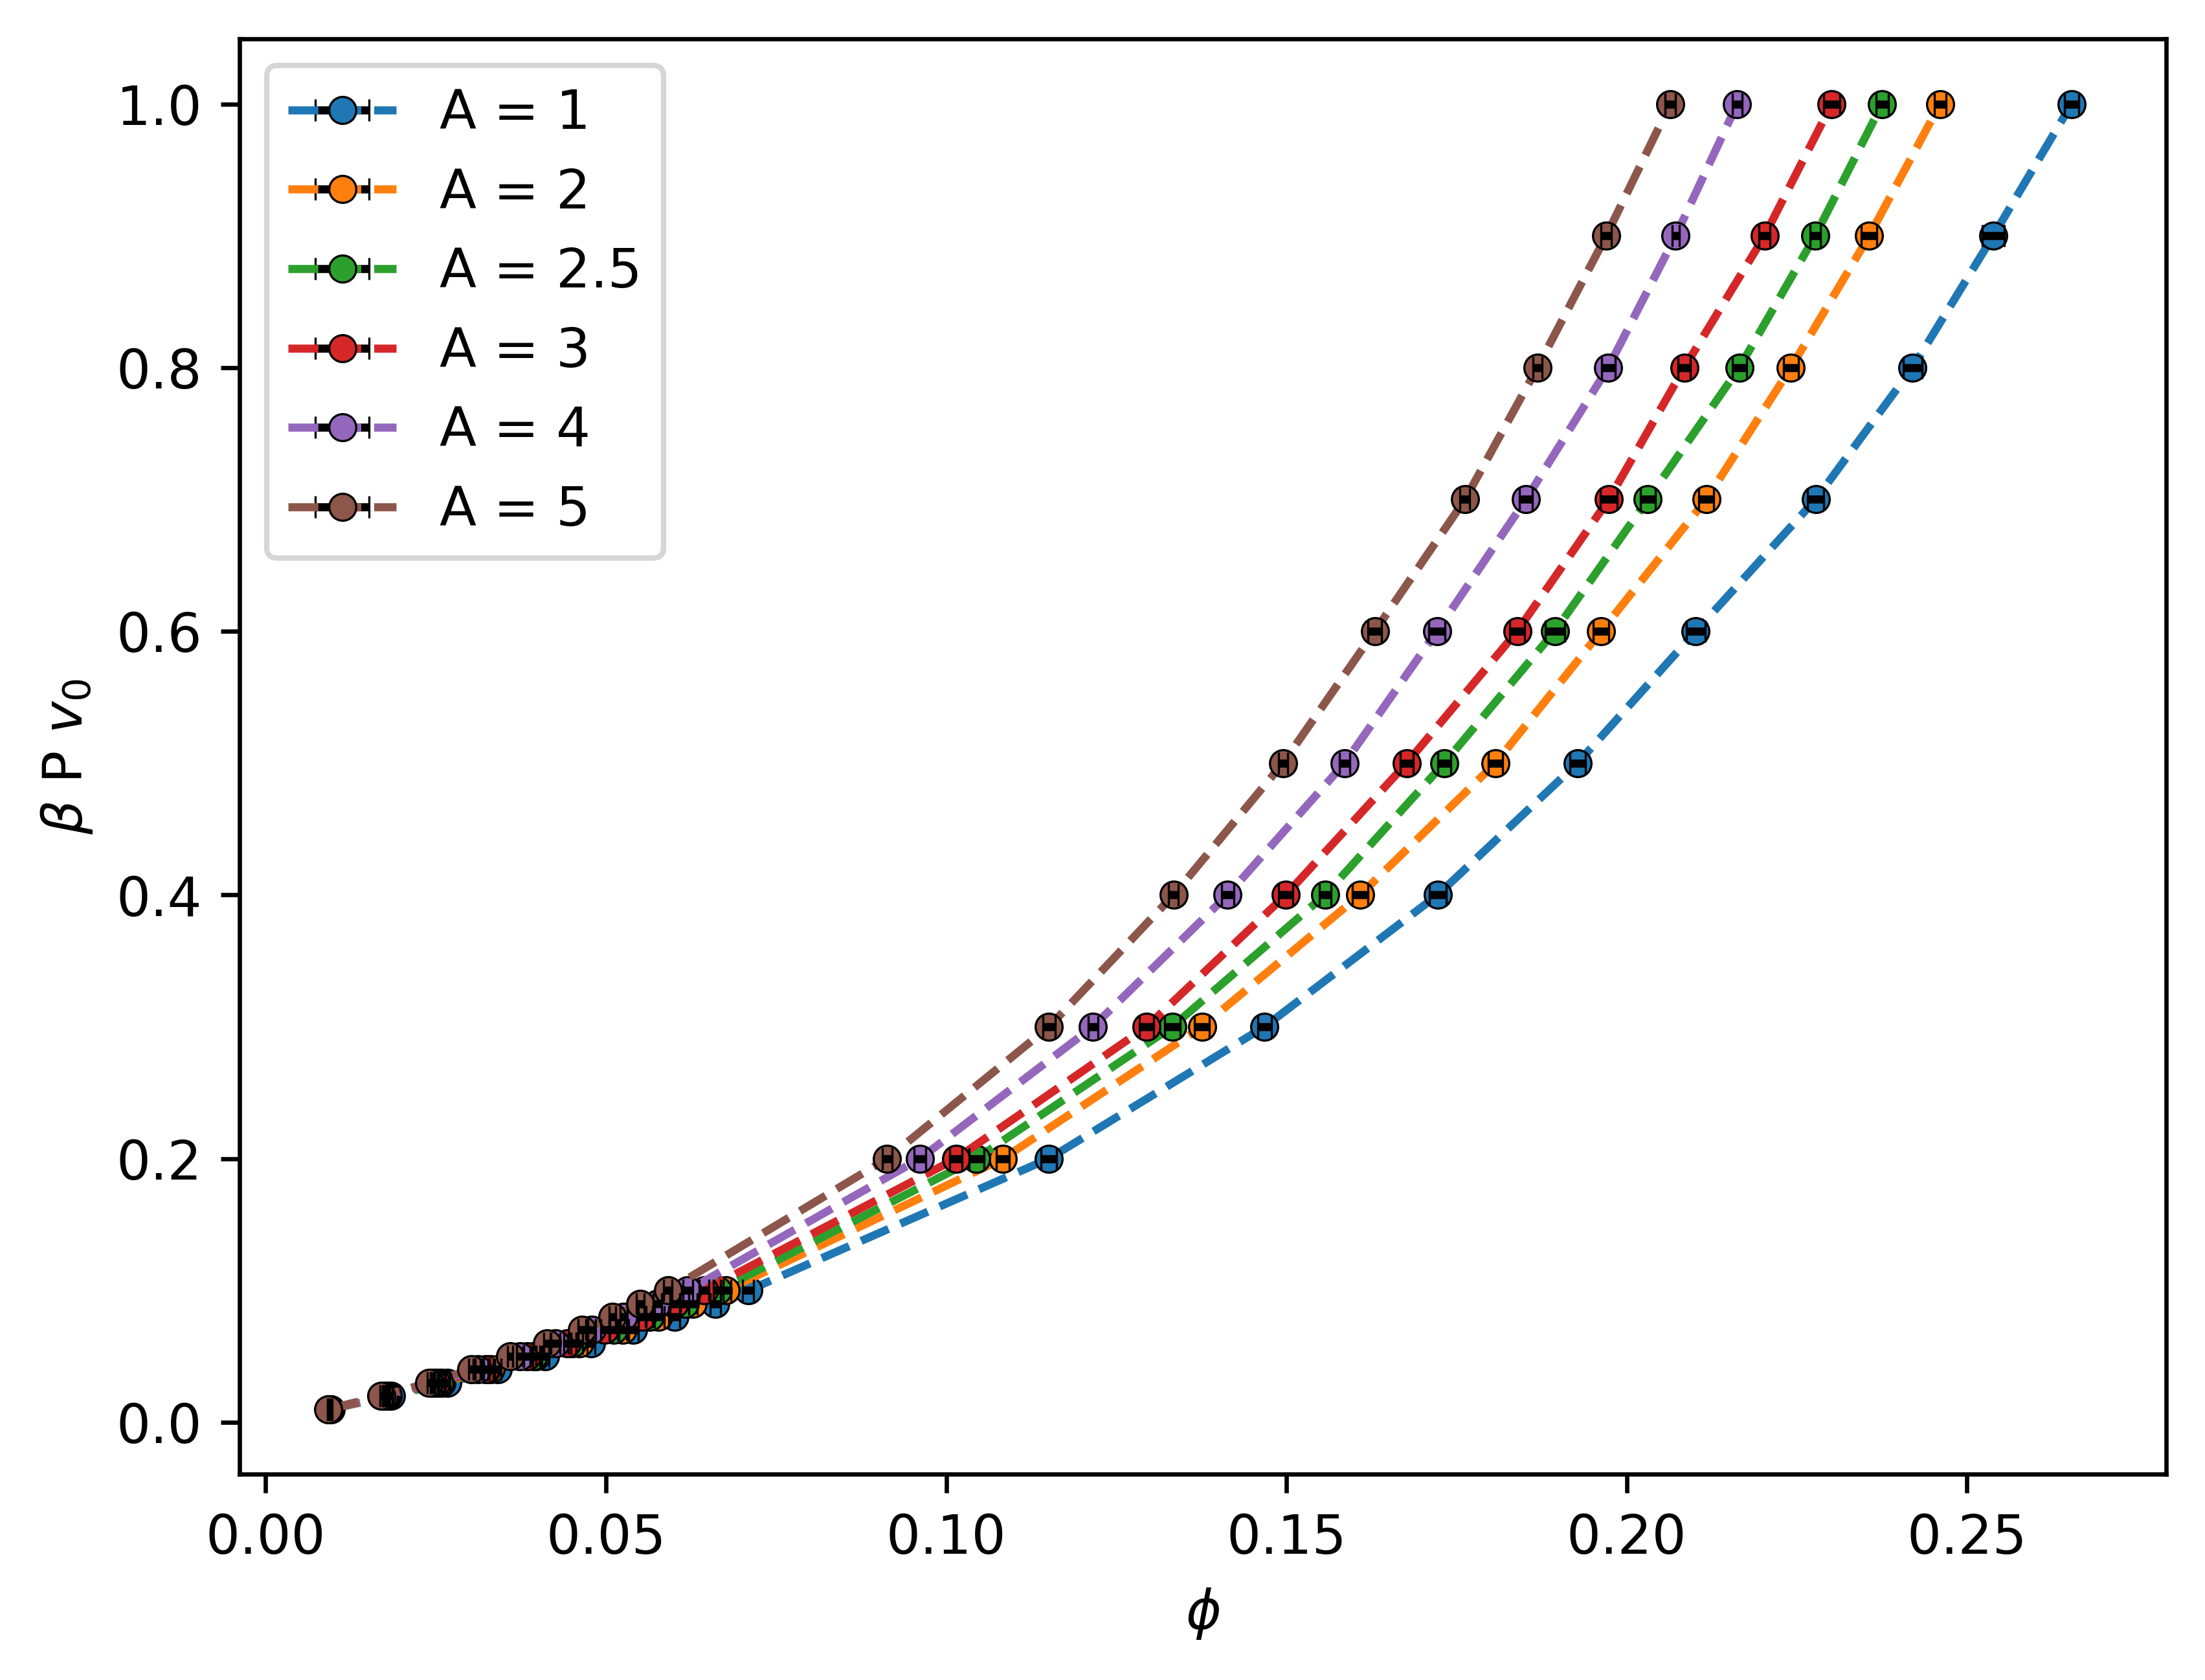
\includegraphics[width=0.3 \columnwidth]{Figures/EOS/Mono.png}
    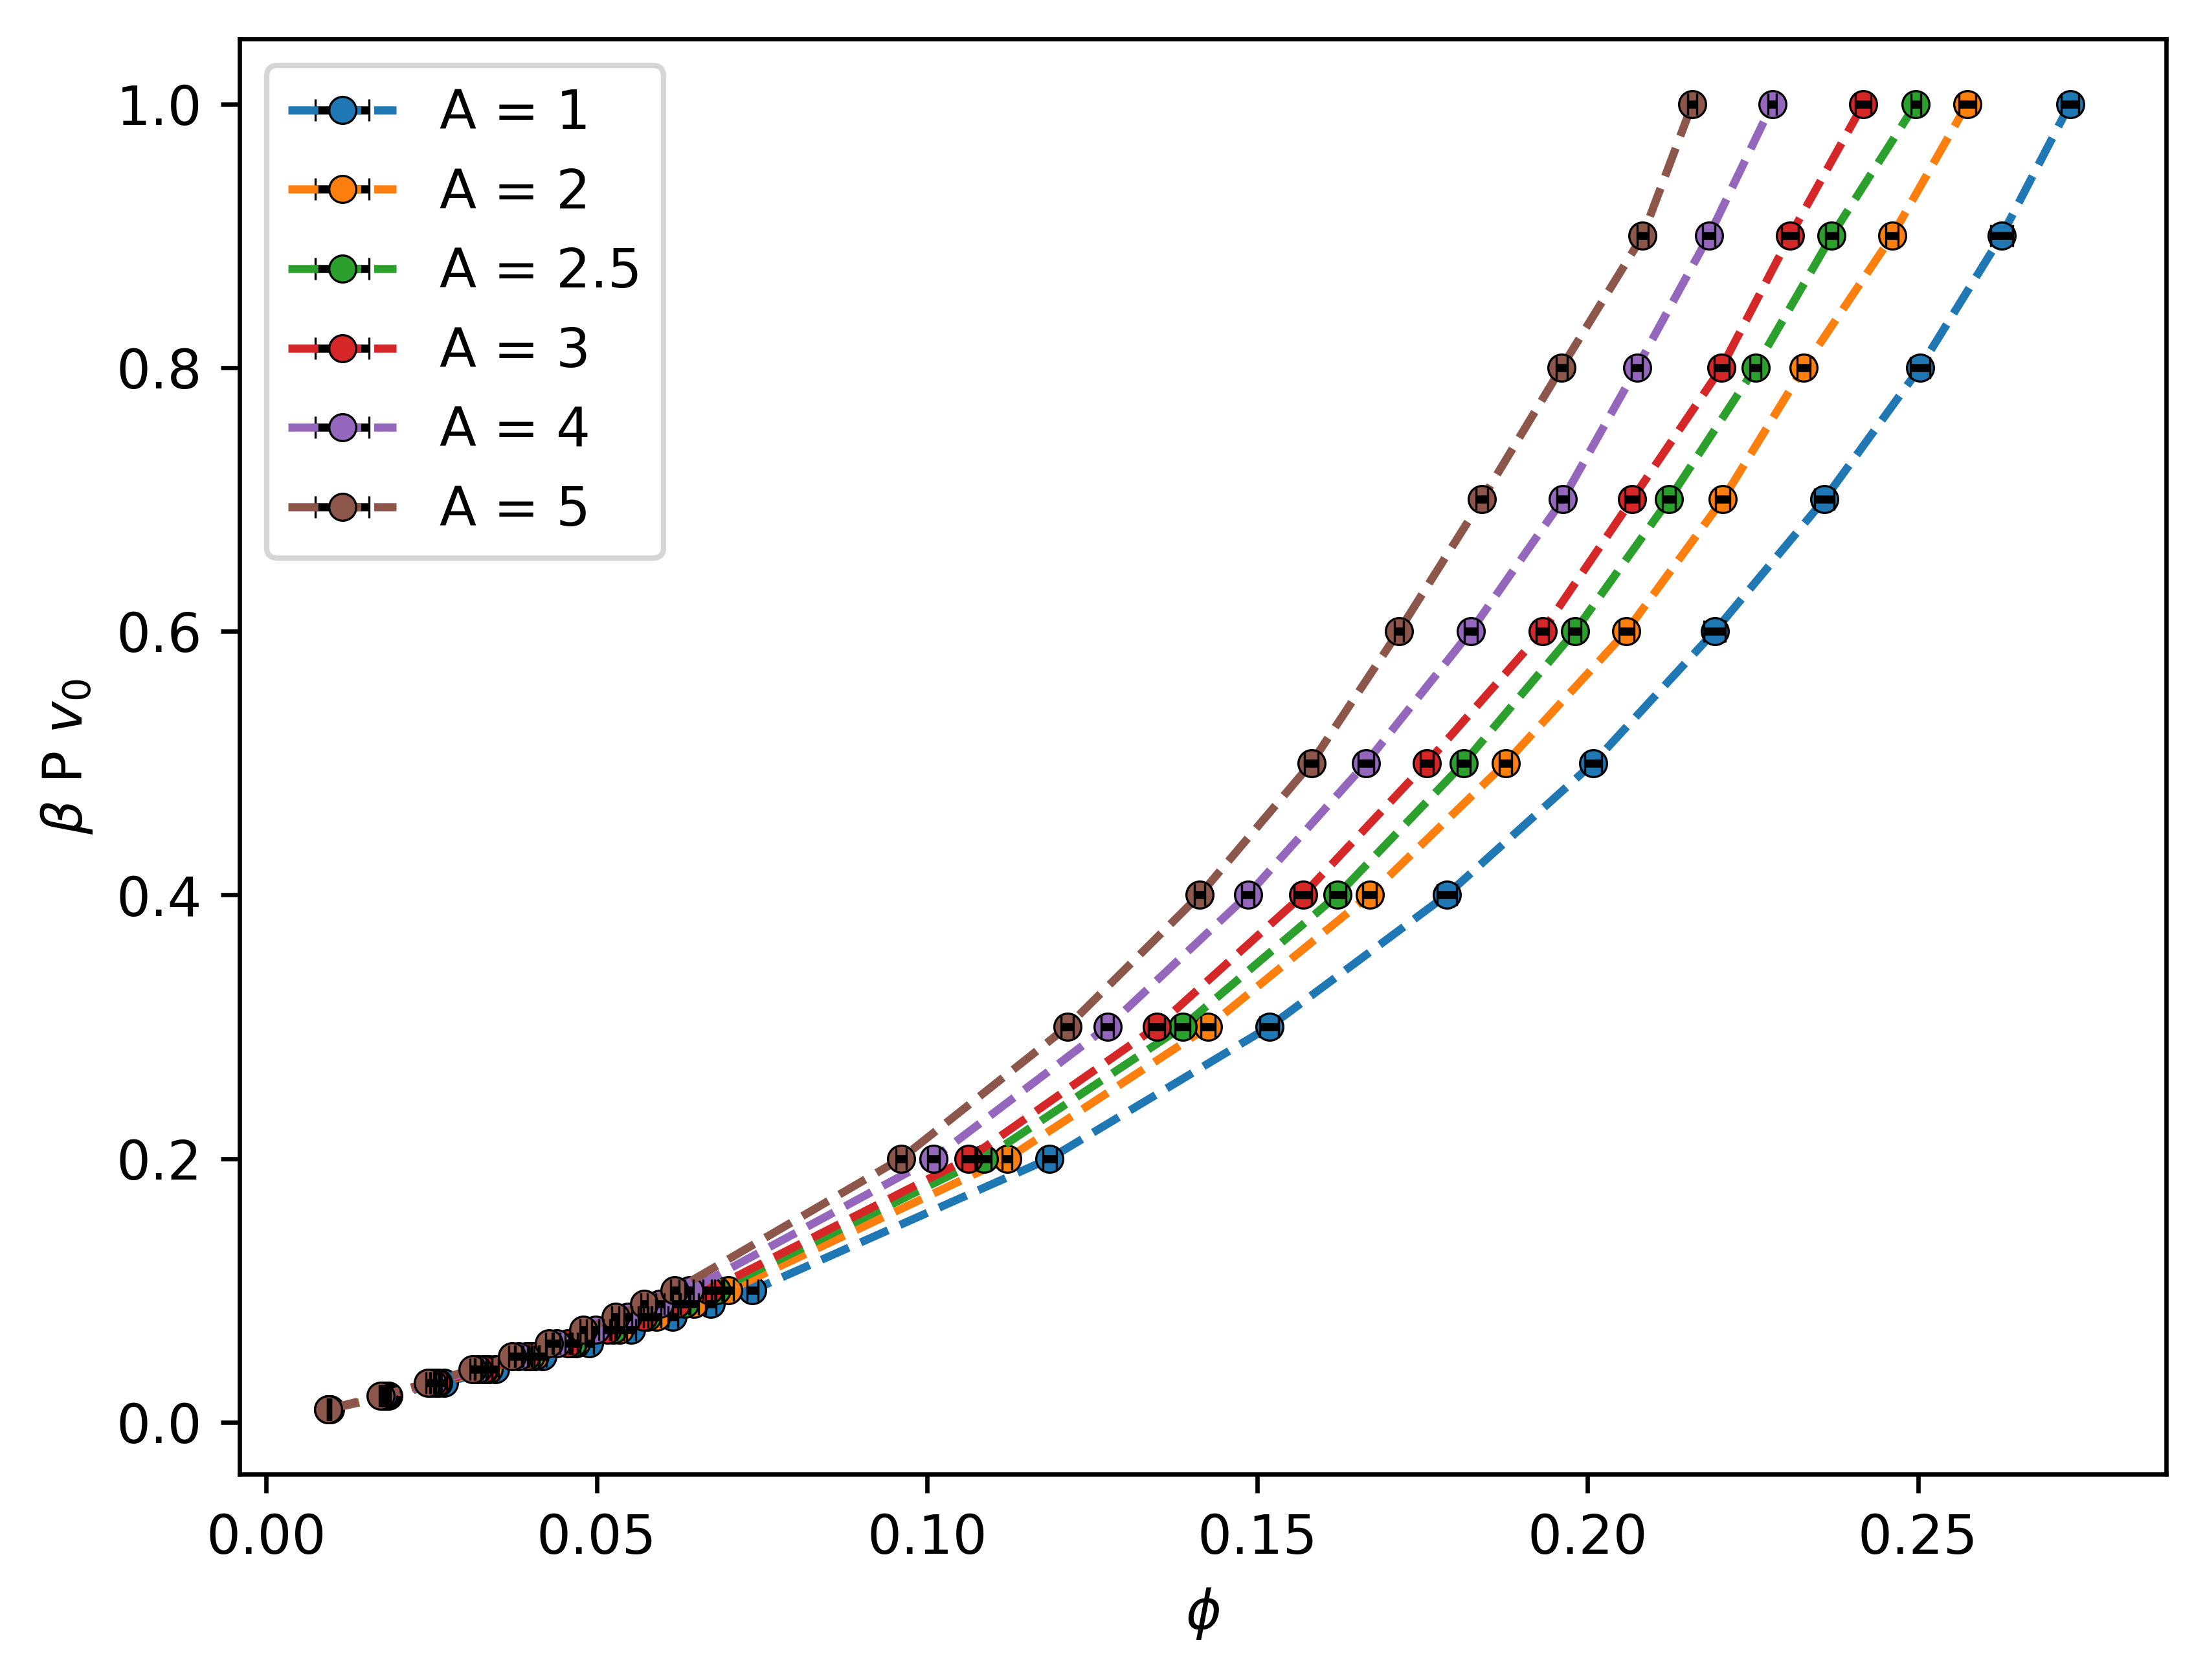
\includegraphics[width=0.3 \columnwidth]{Figures/EOS/PolyD.png}
    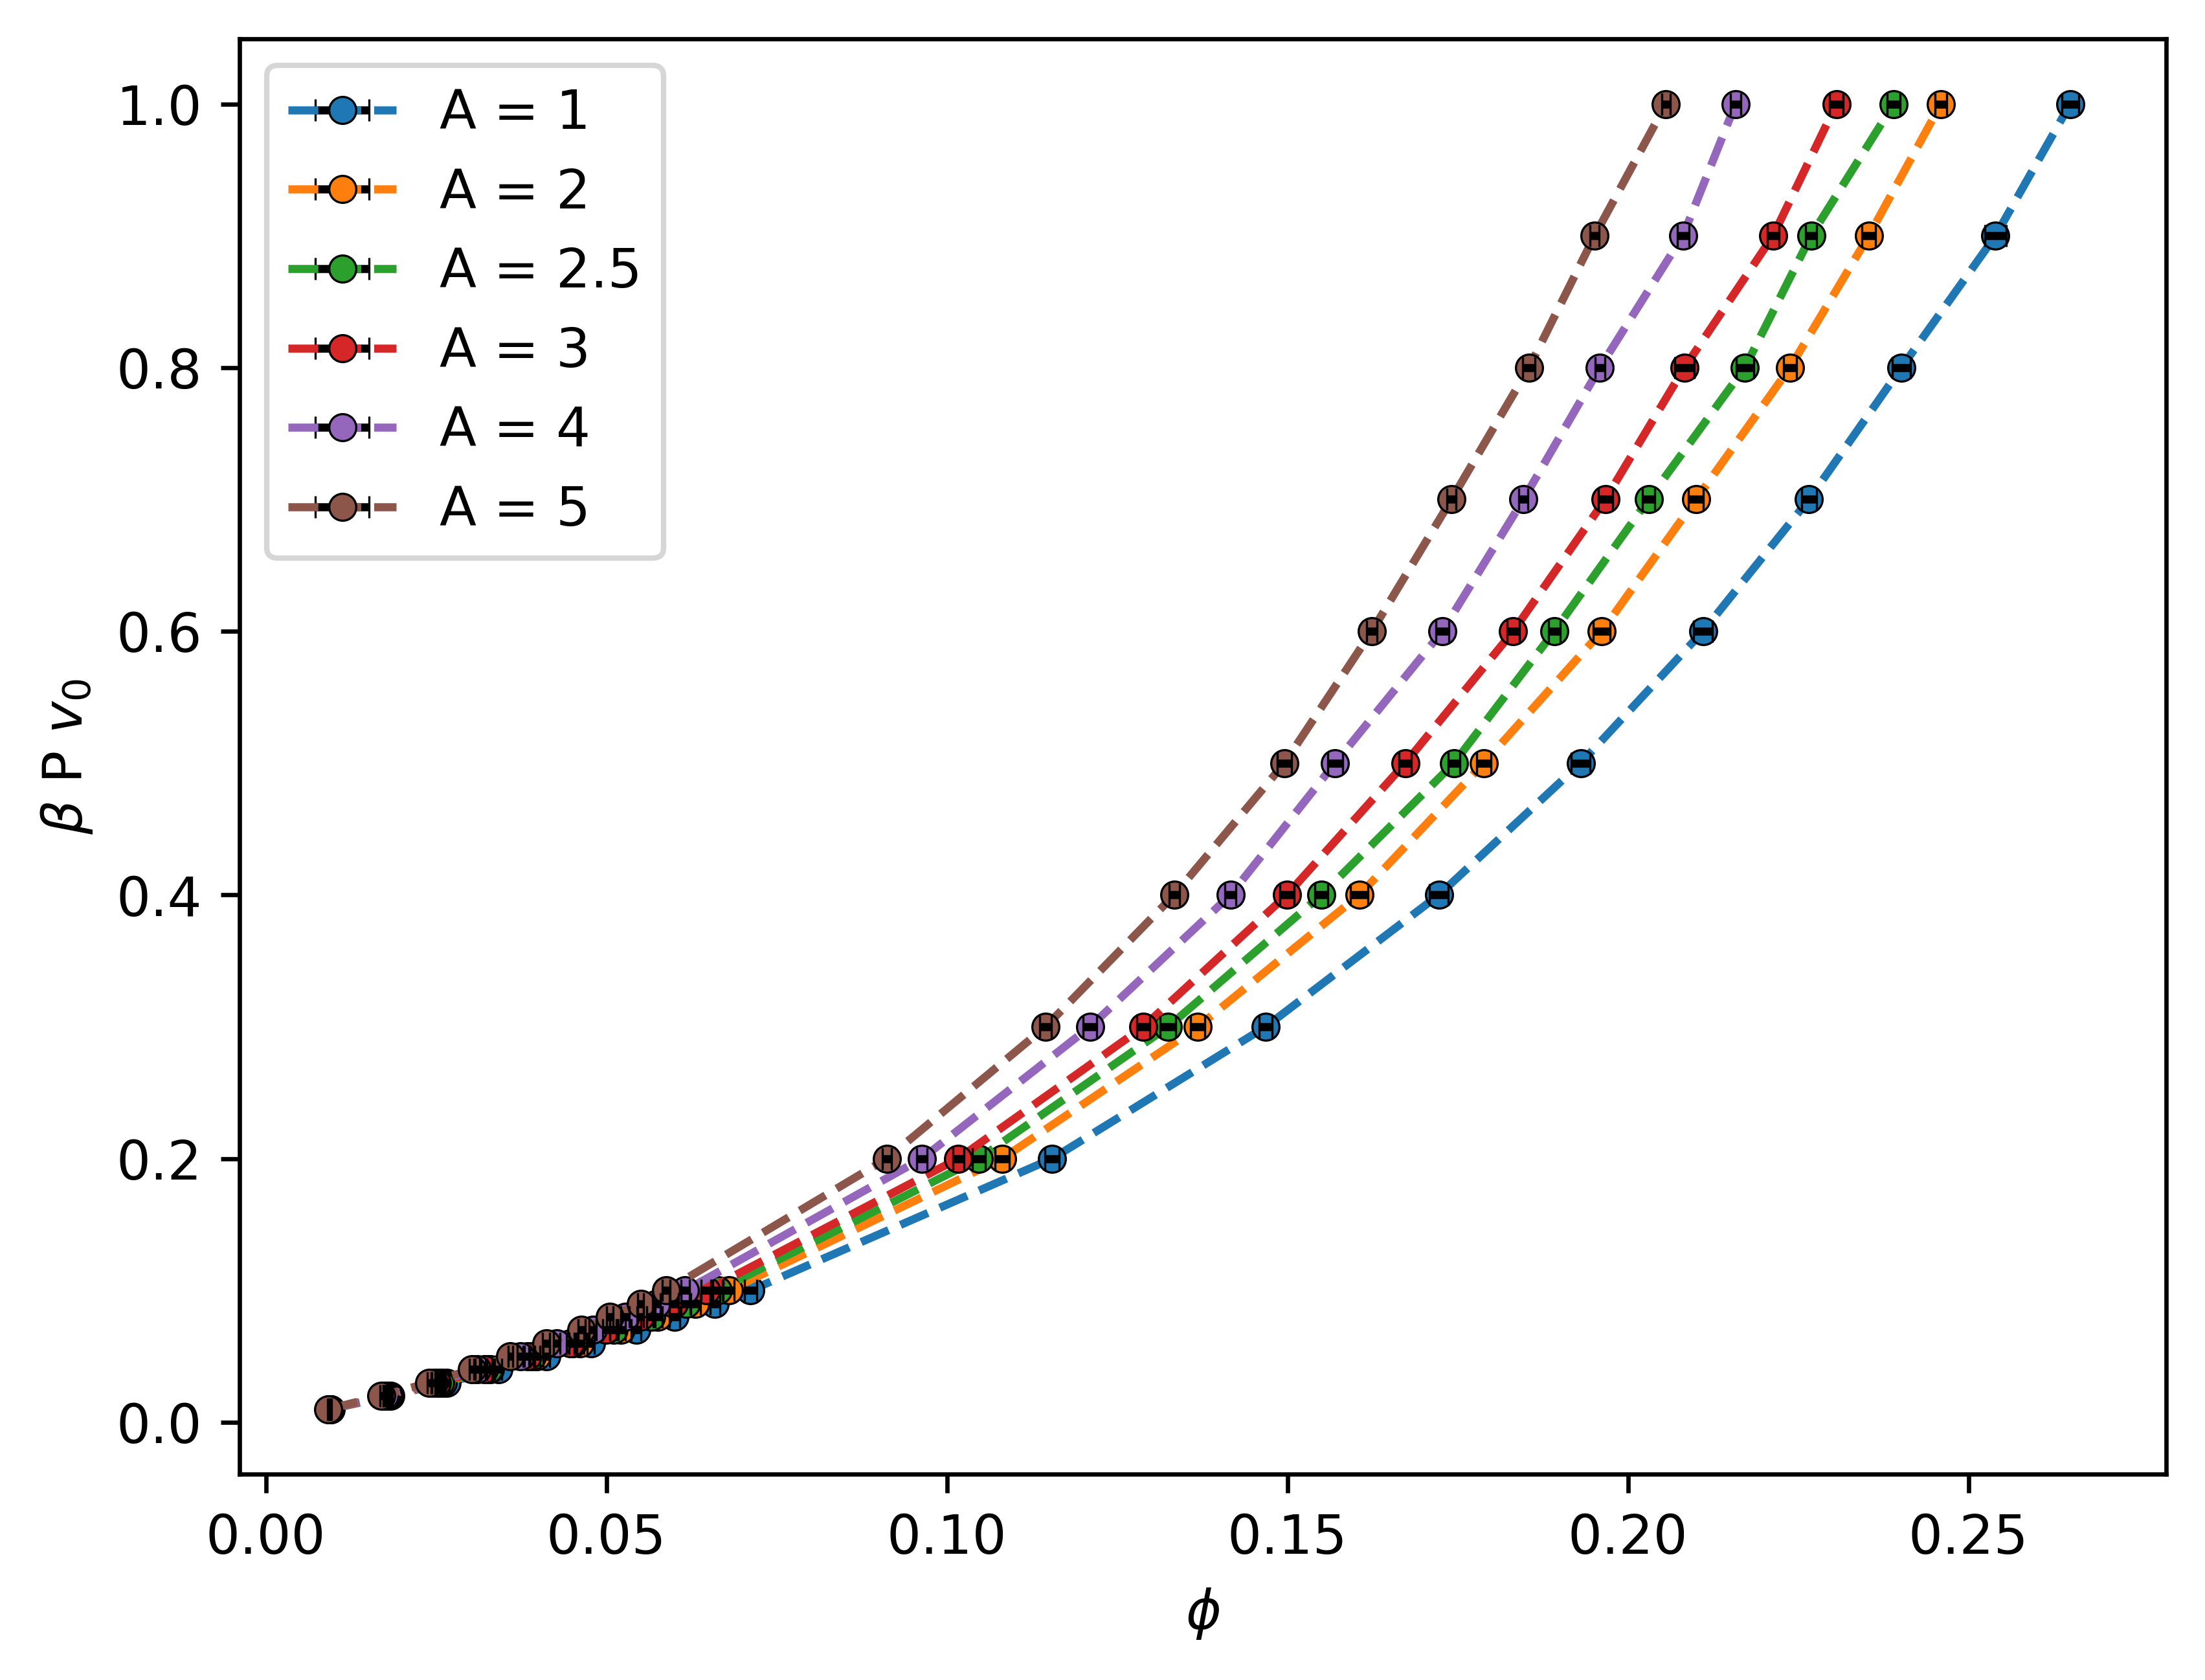
\includegraphics[width=0.3 \columnwidth]{Figures/EOS/PolyL.png}
    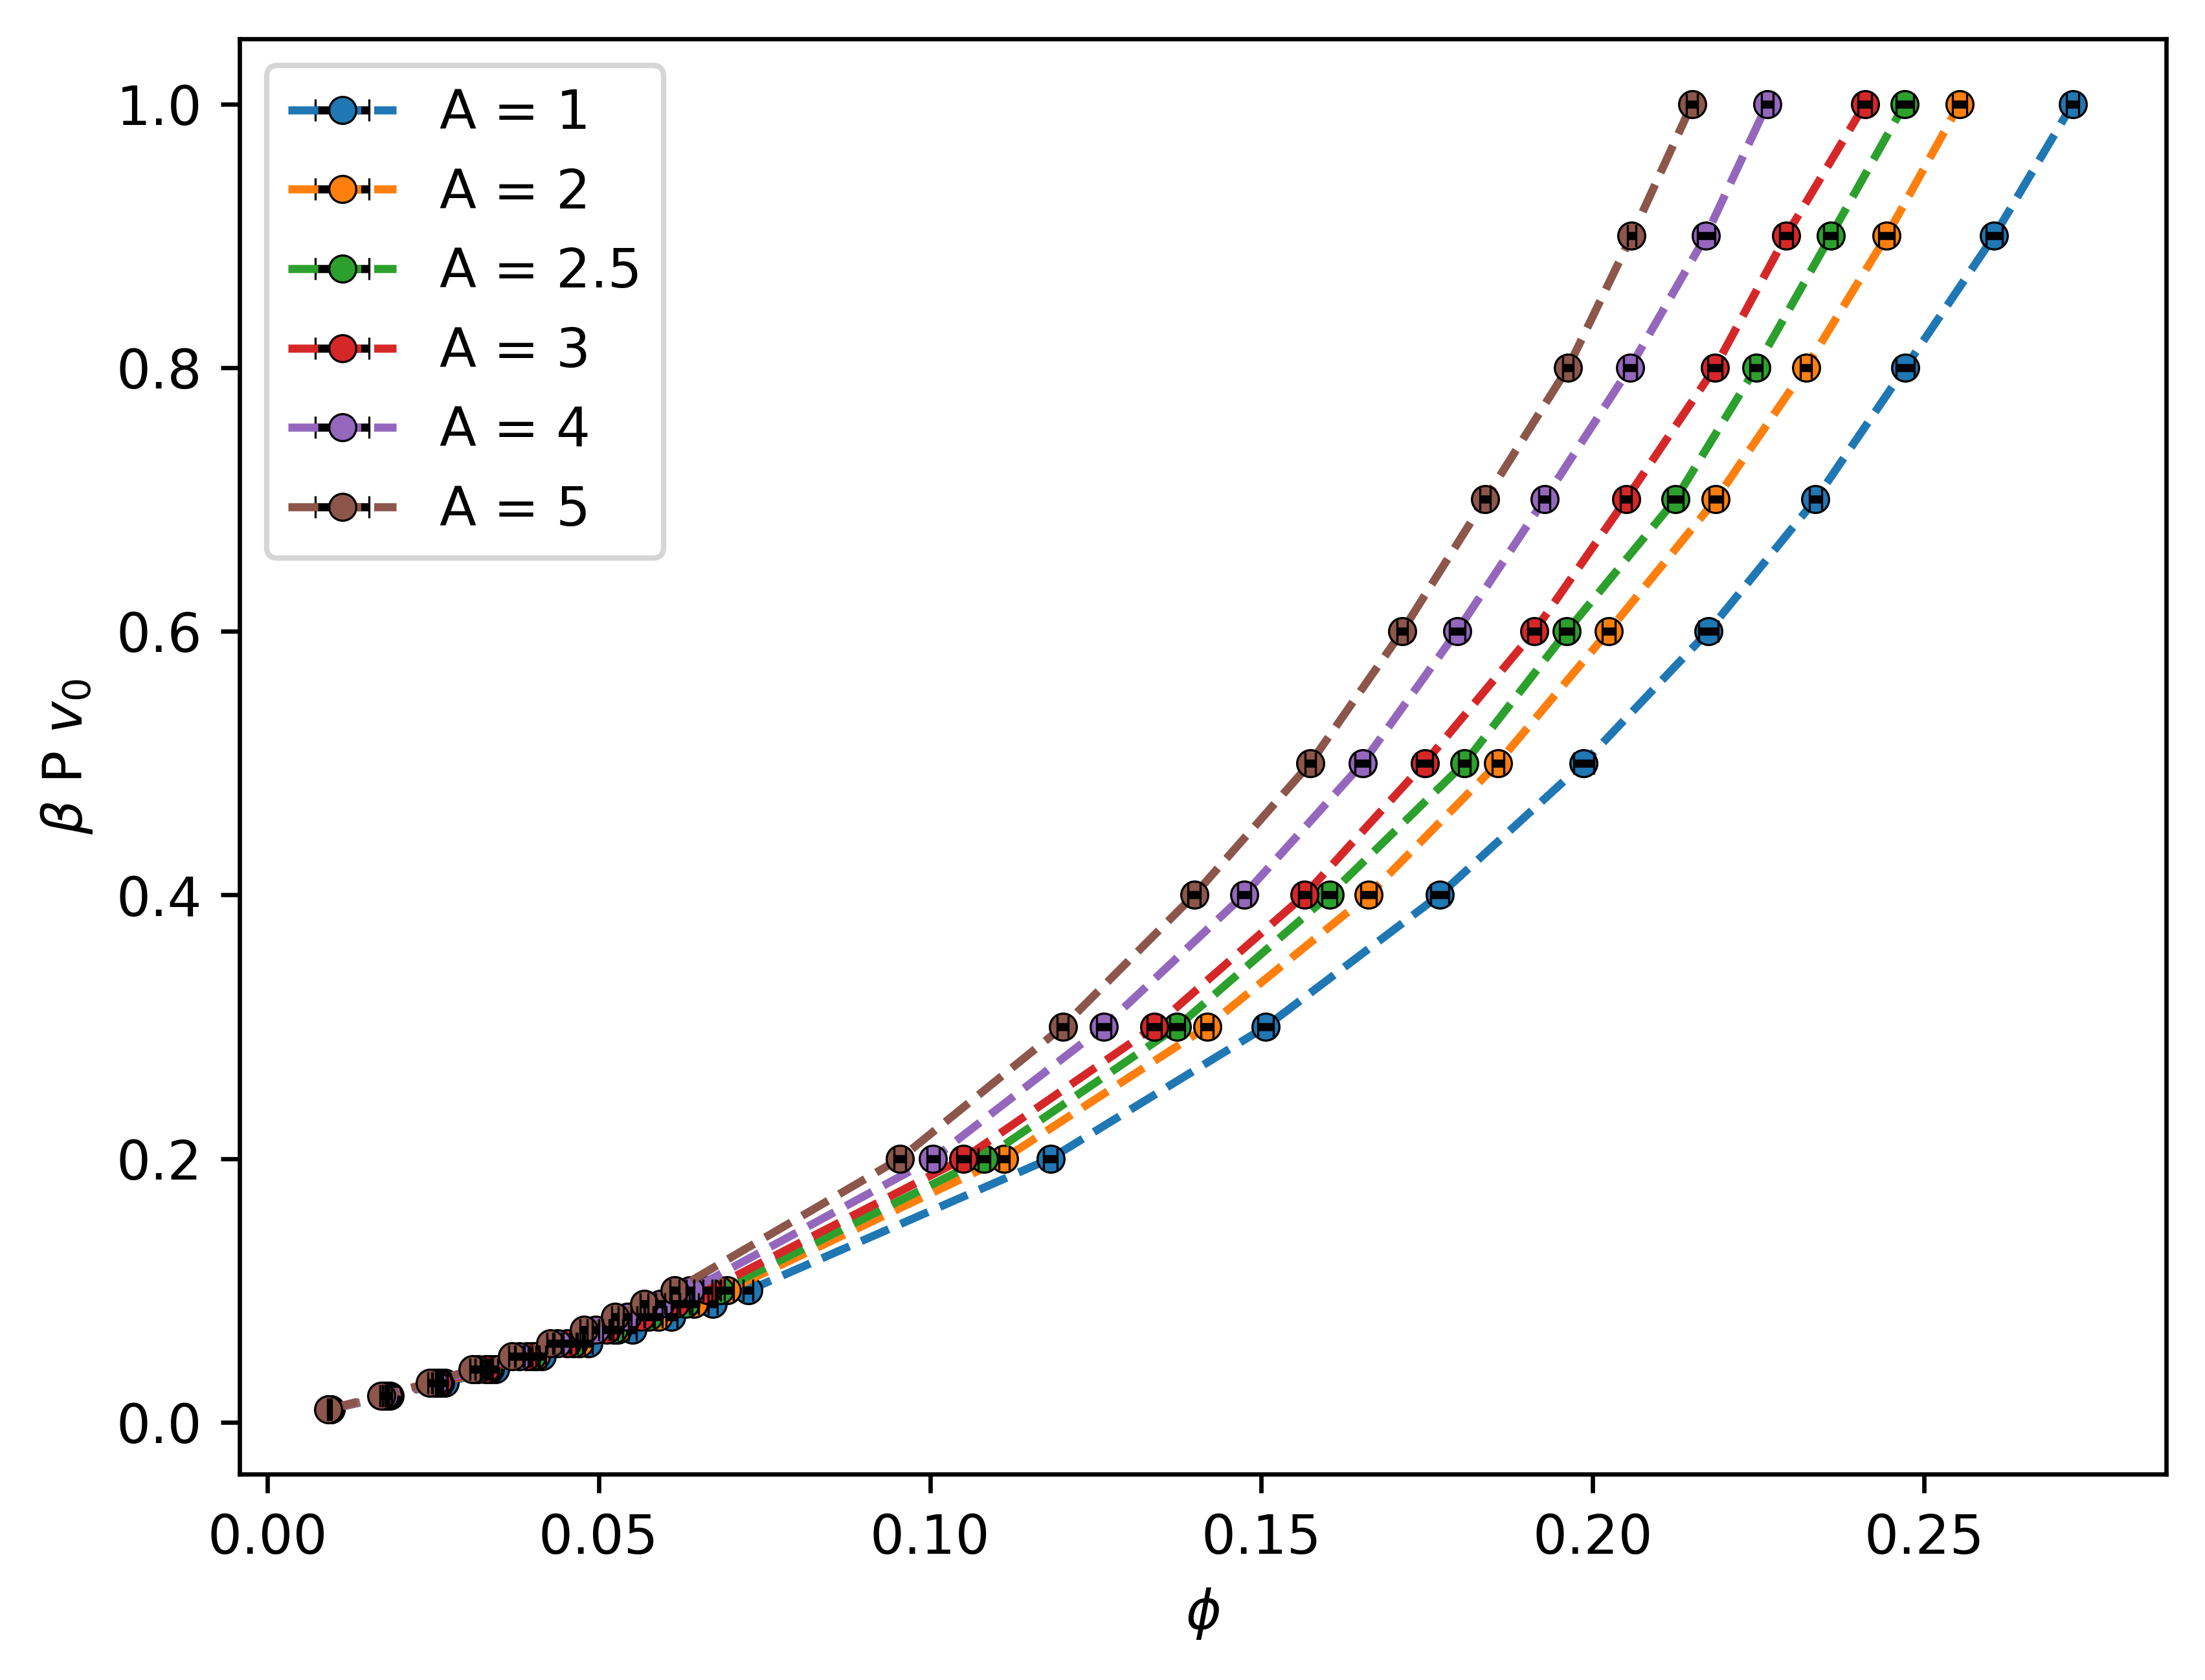
\includegraphics[width=0.3 \columnwidth]{Figures/EOS/PolyDGauss.png}
    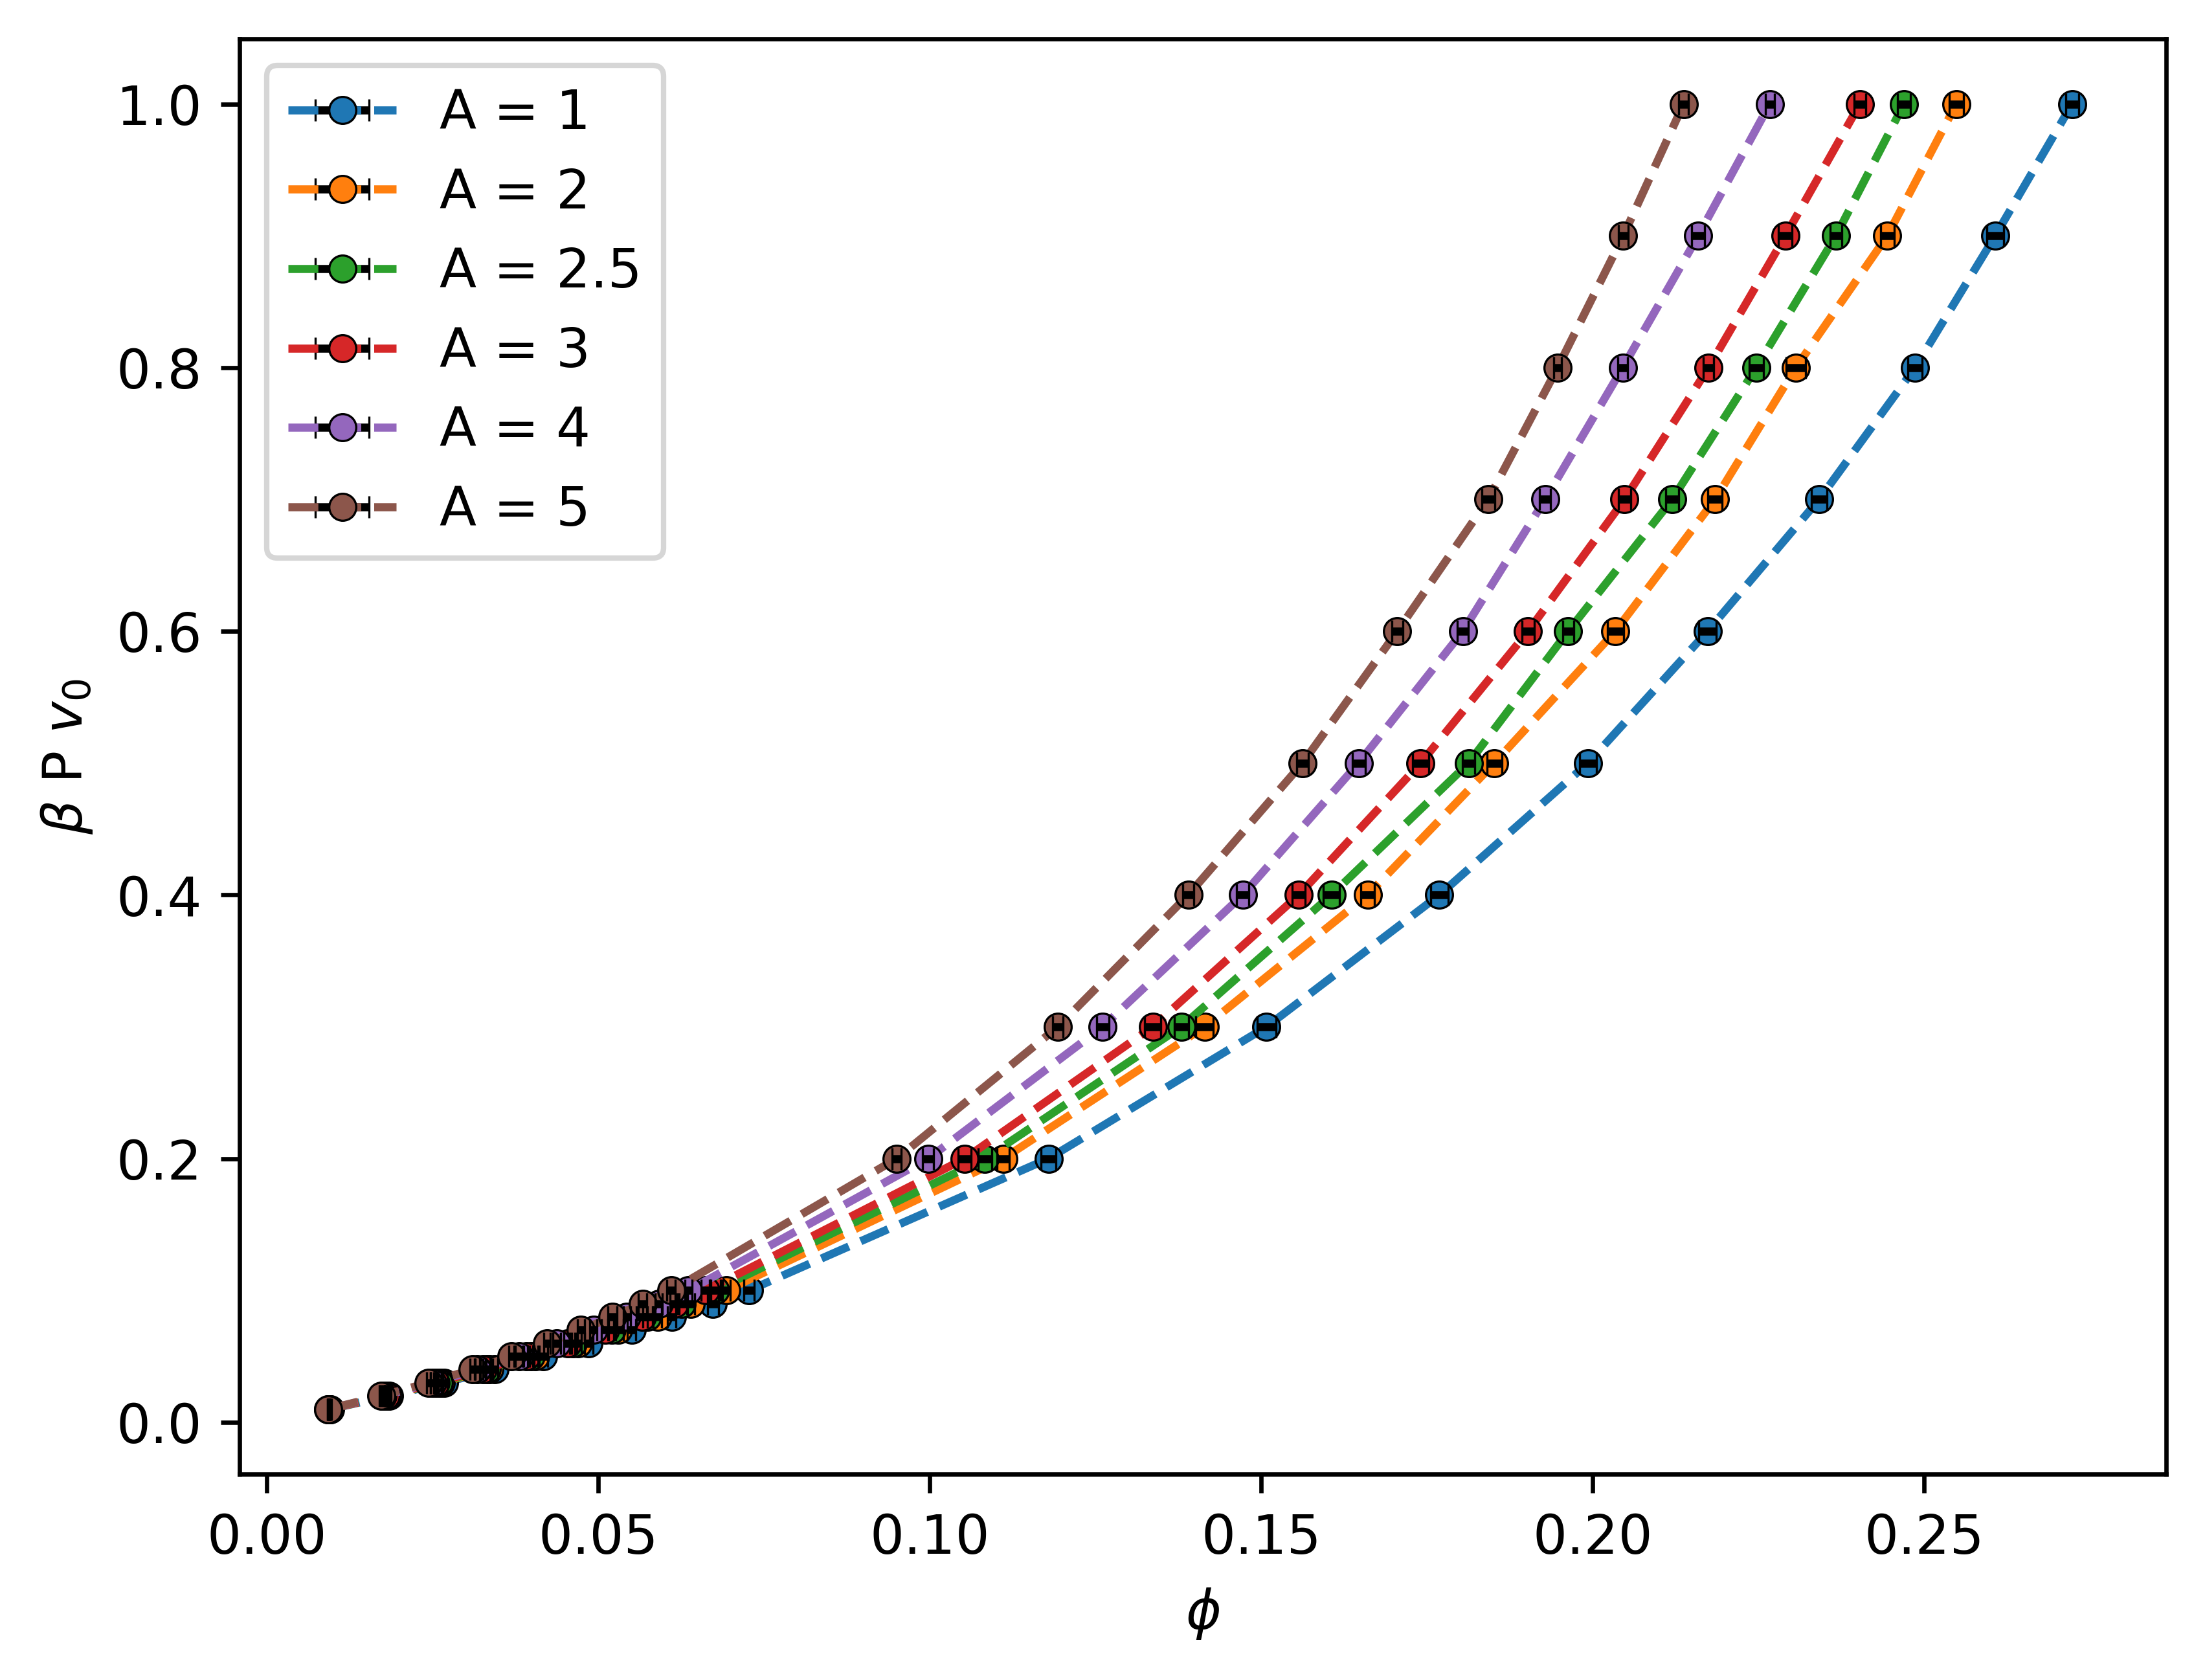
\includegraphics[width=0.3 \columnwidth]{Figures/EOS/PolyDLGauss.png}
    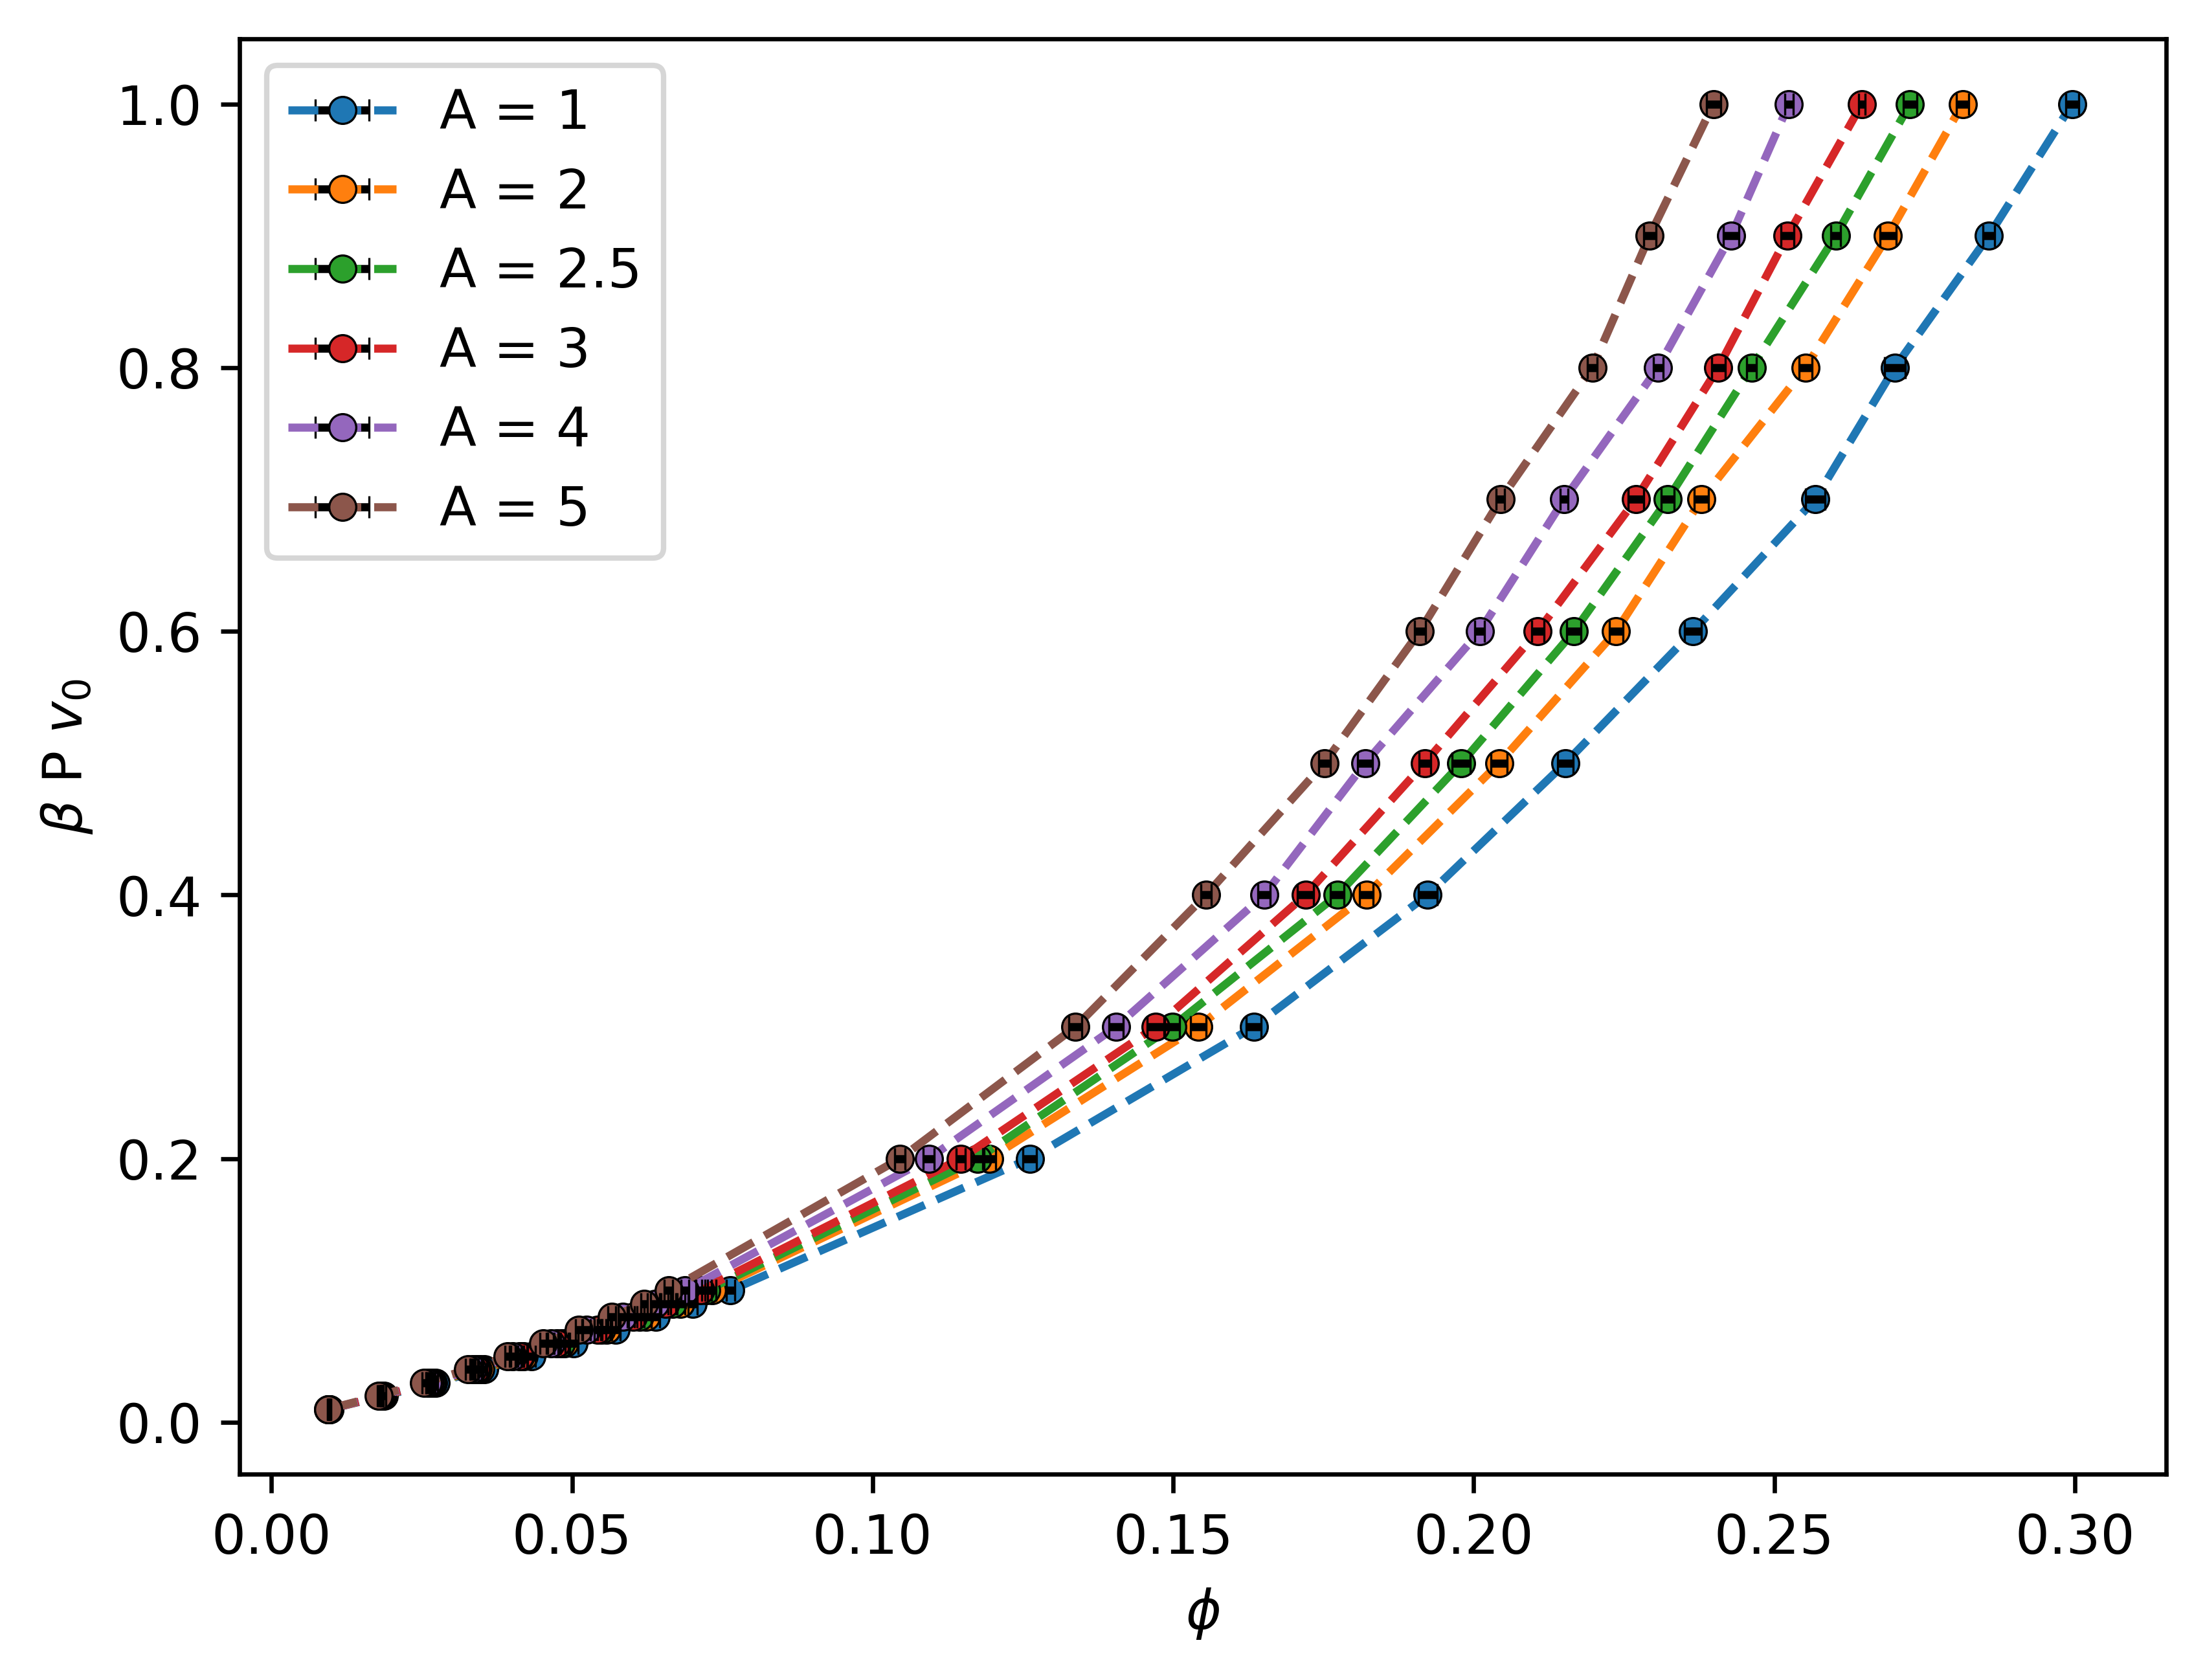
\includegraphics[width=0.3 \columnwidth]{Figures/EOS/PolyD0.75.png}
    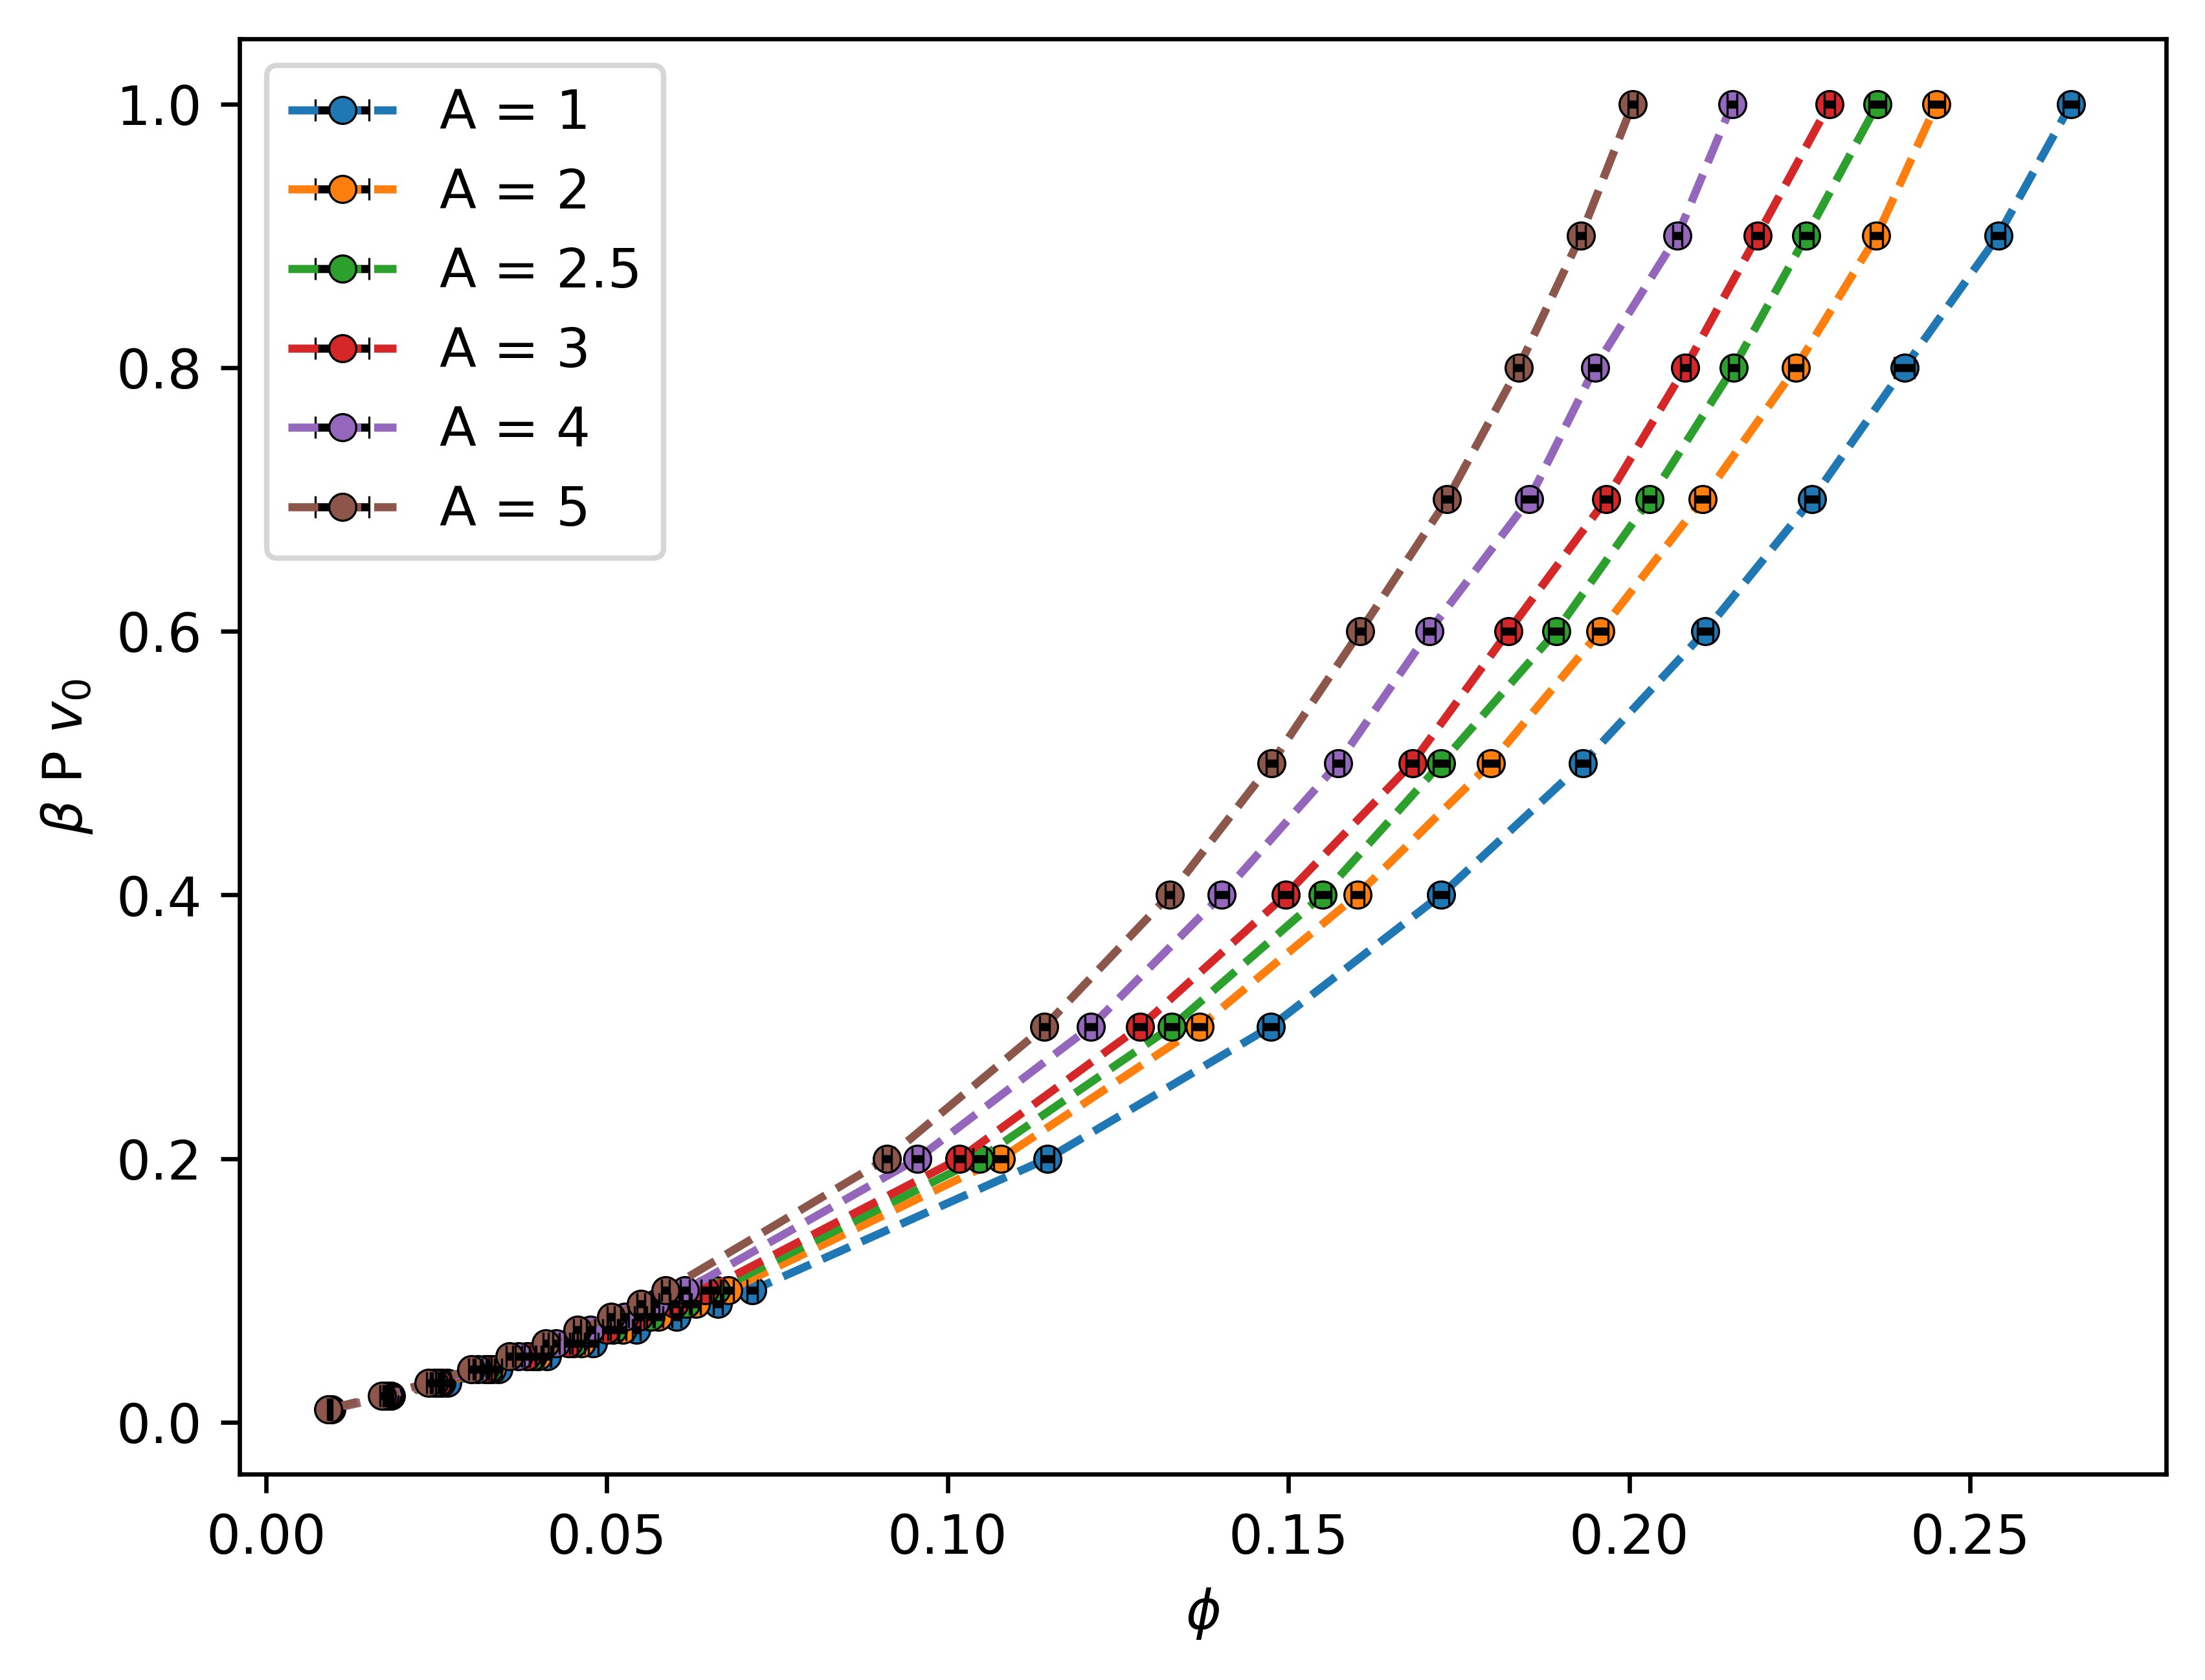
\includegraphics[width=0.3 \columnwidth]{Figures/EOS/PolyL0.75}
    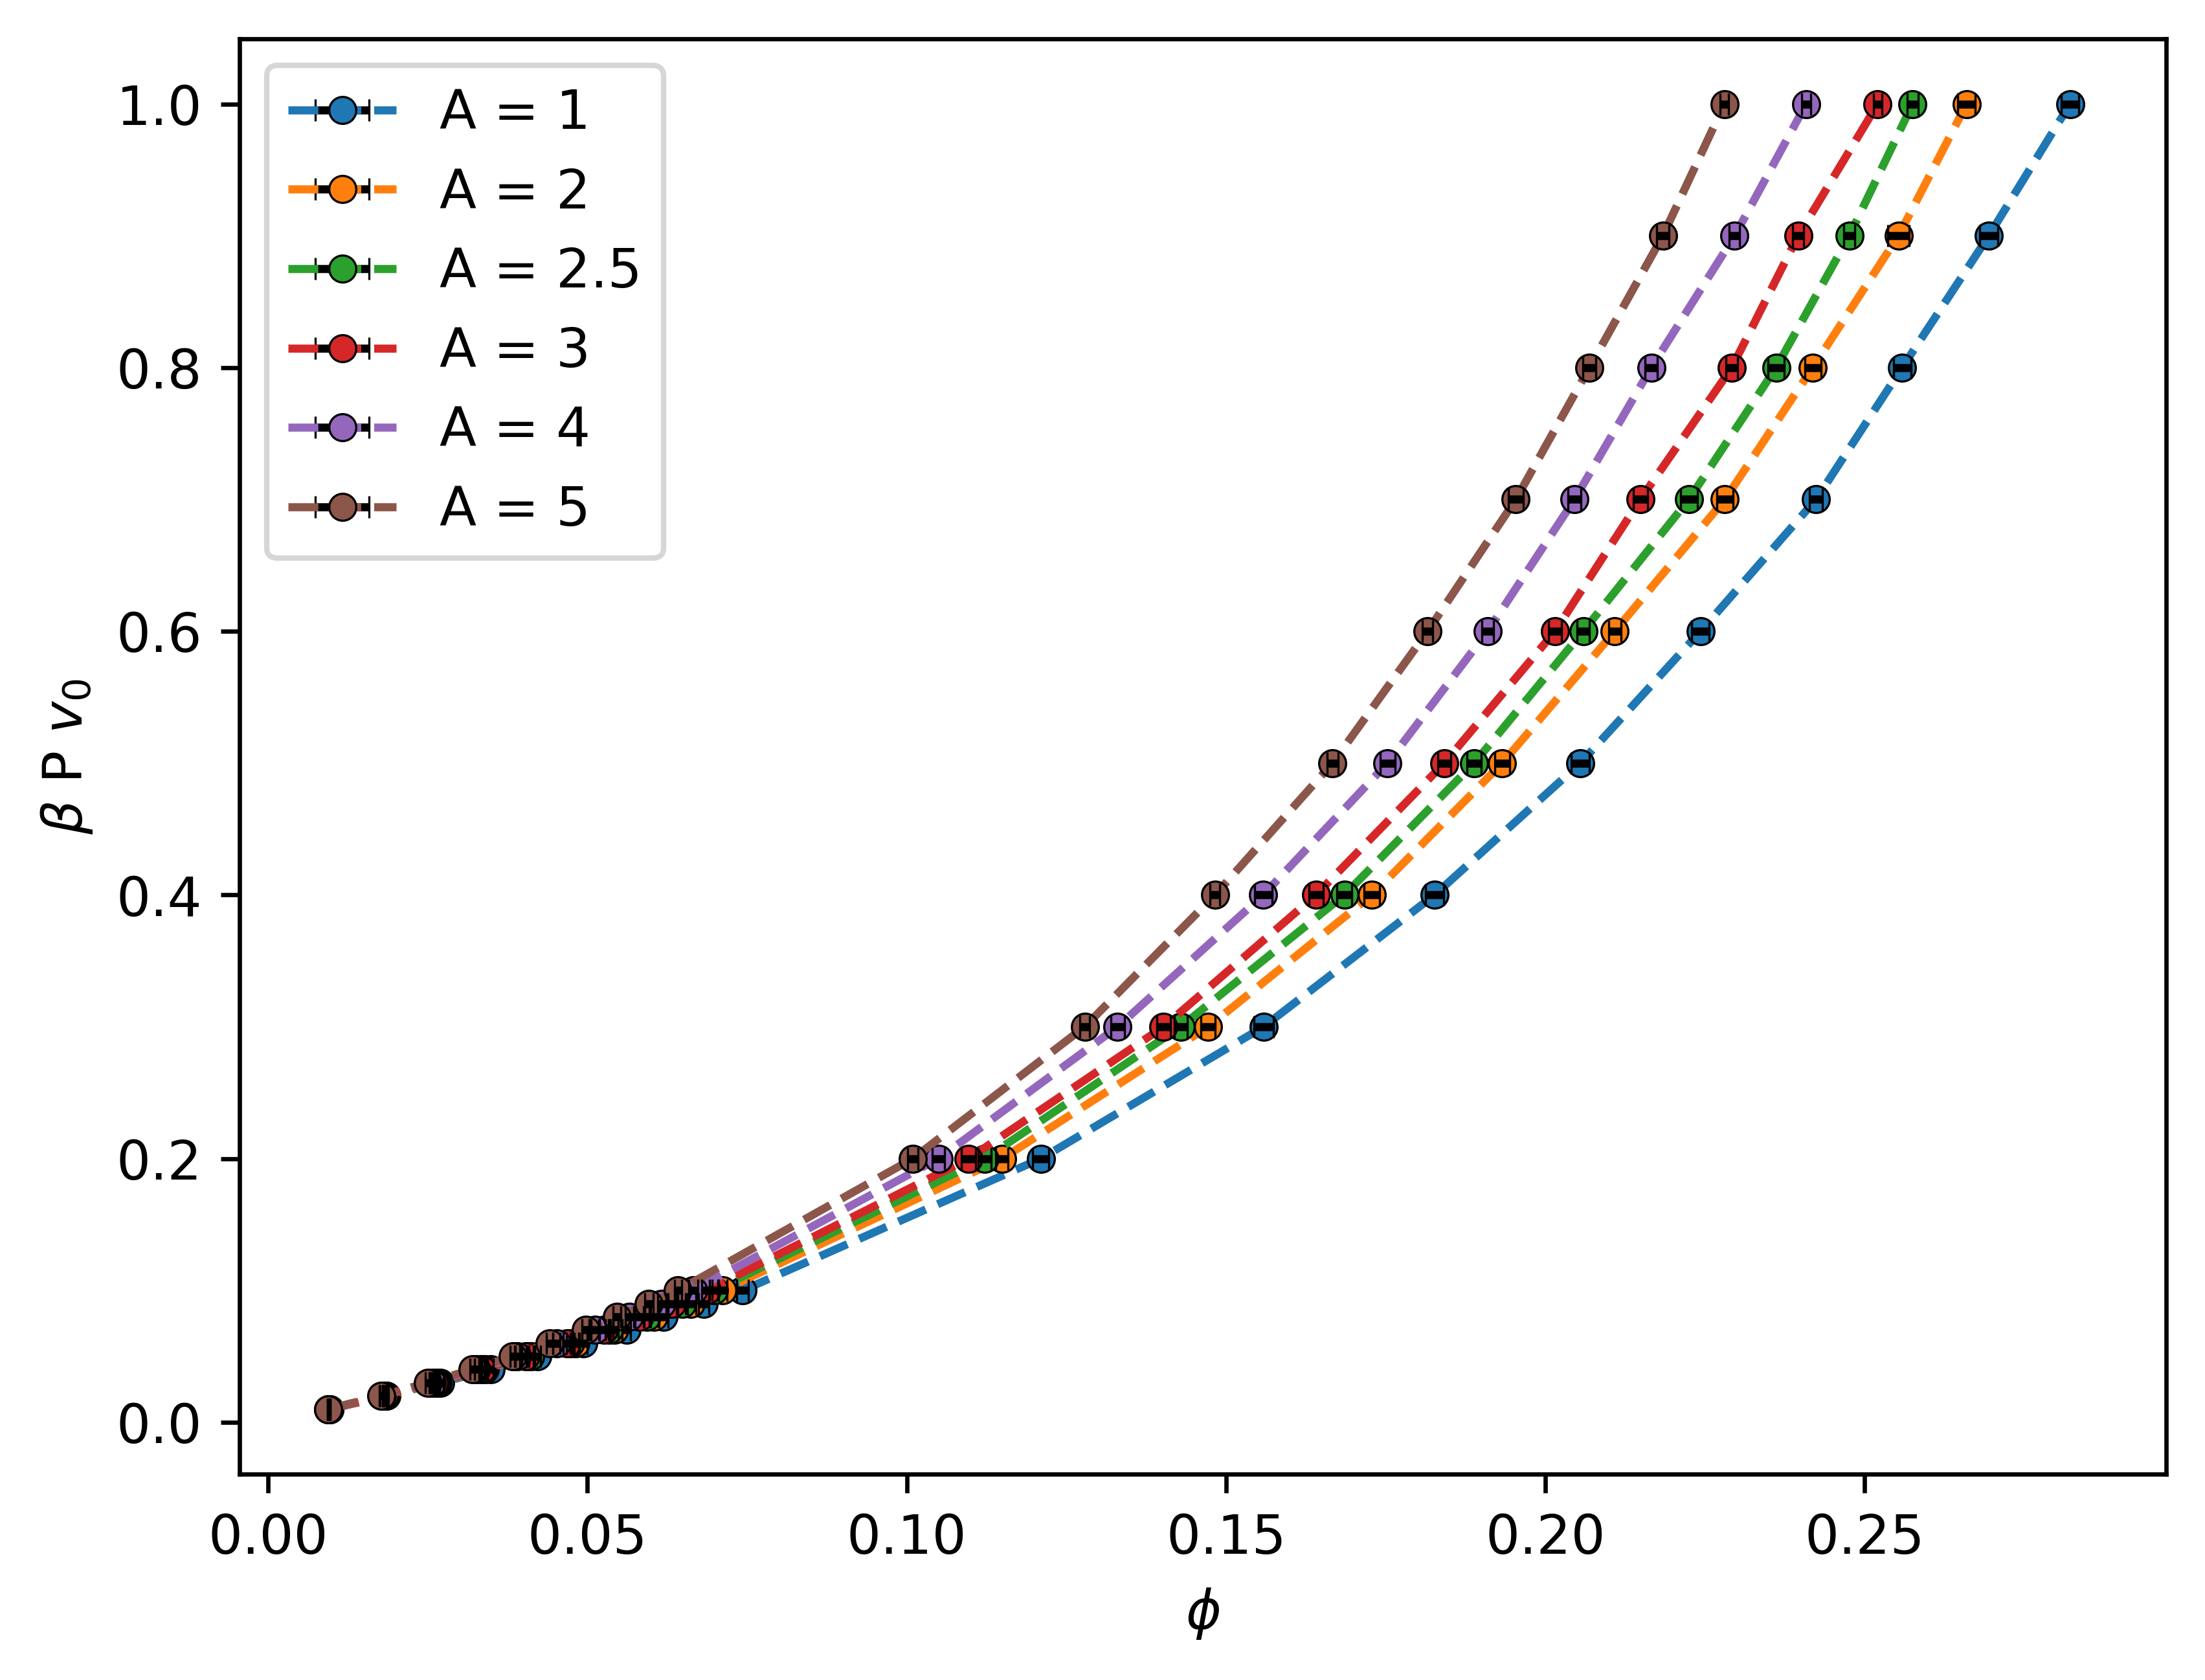
\includegraphics[width=0.3 \columnwidth]{Figures/EOS/PolyDGauss0.75.png}
    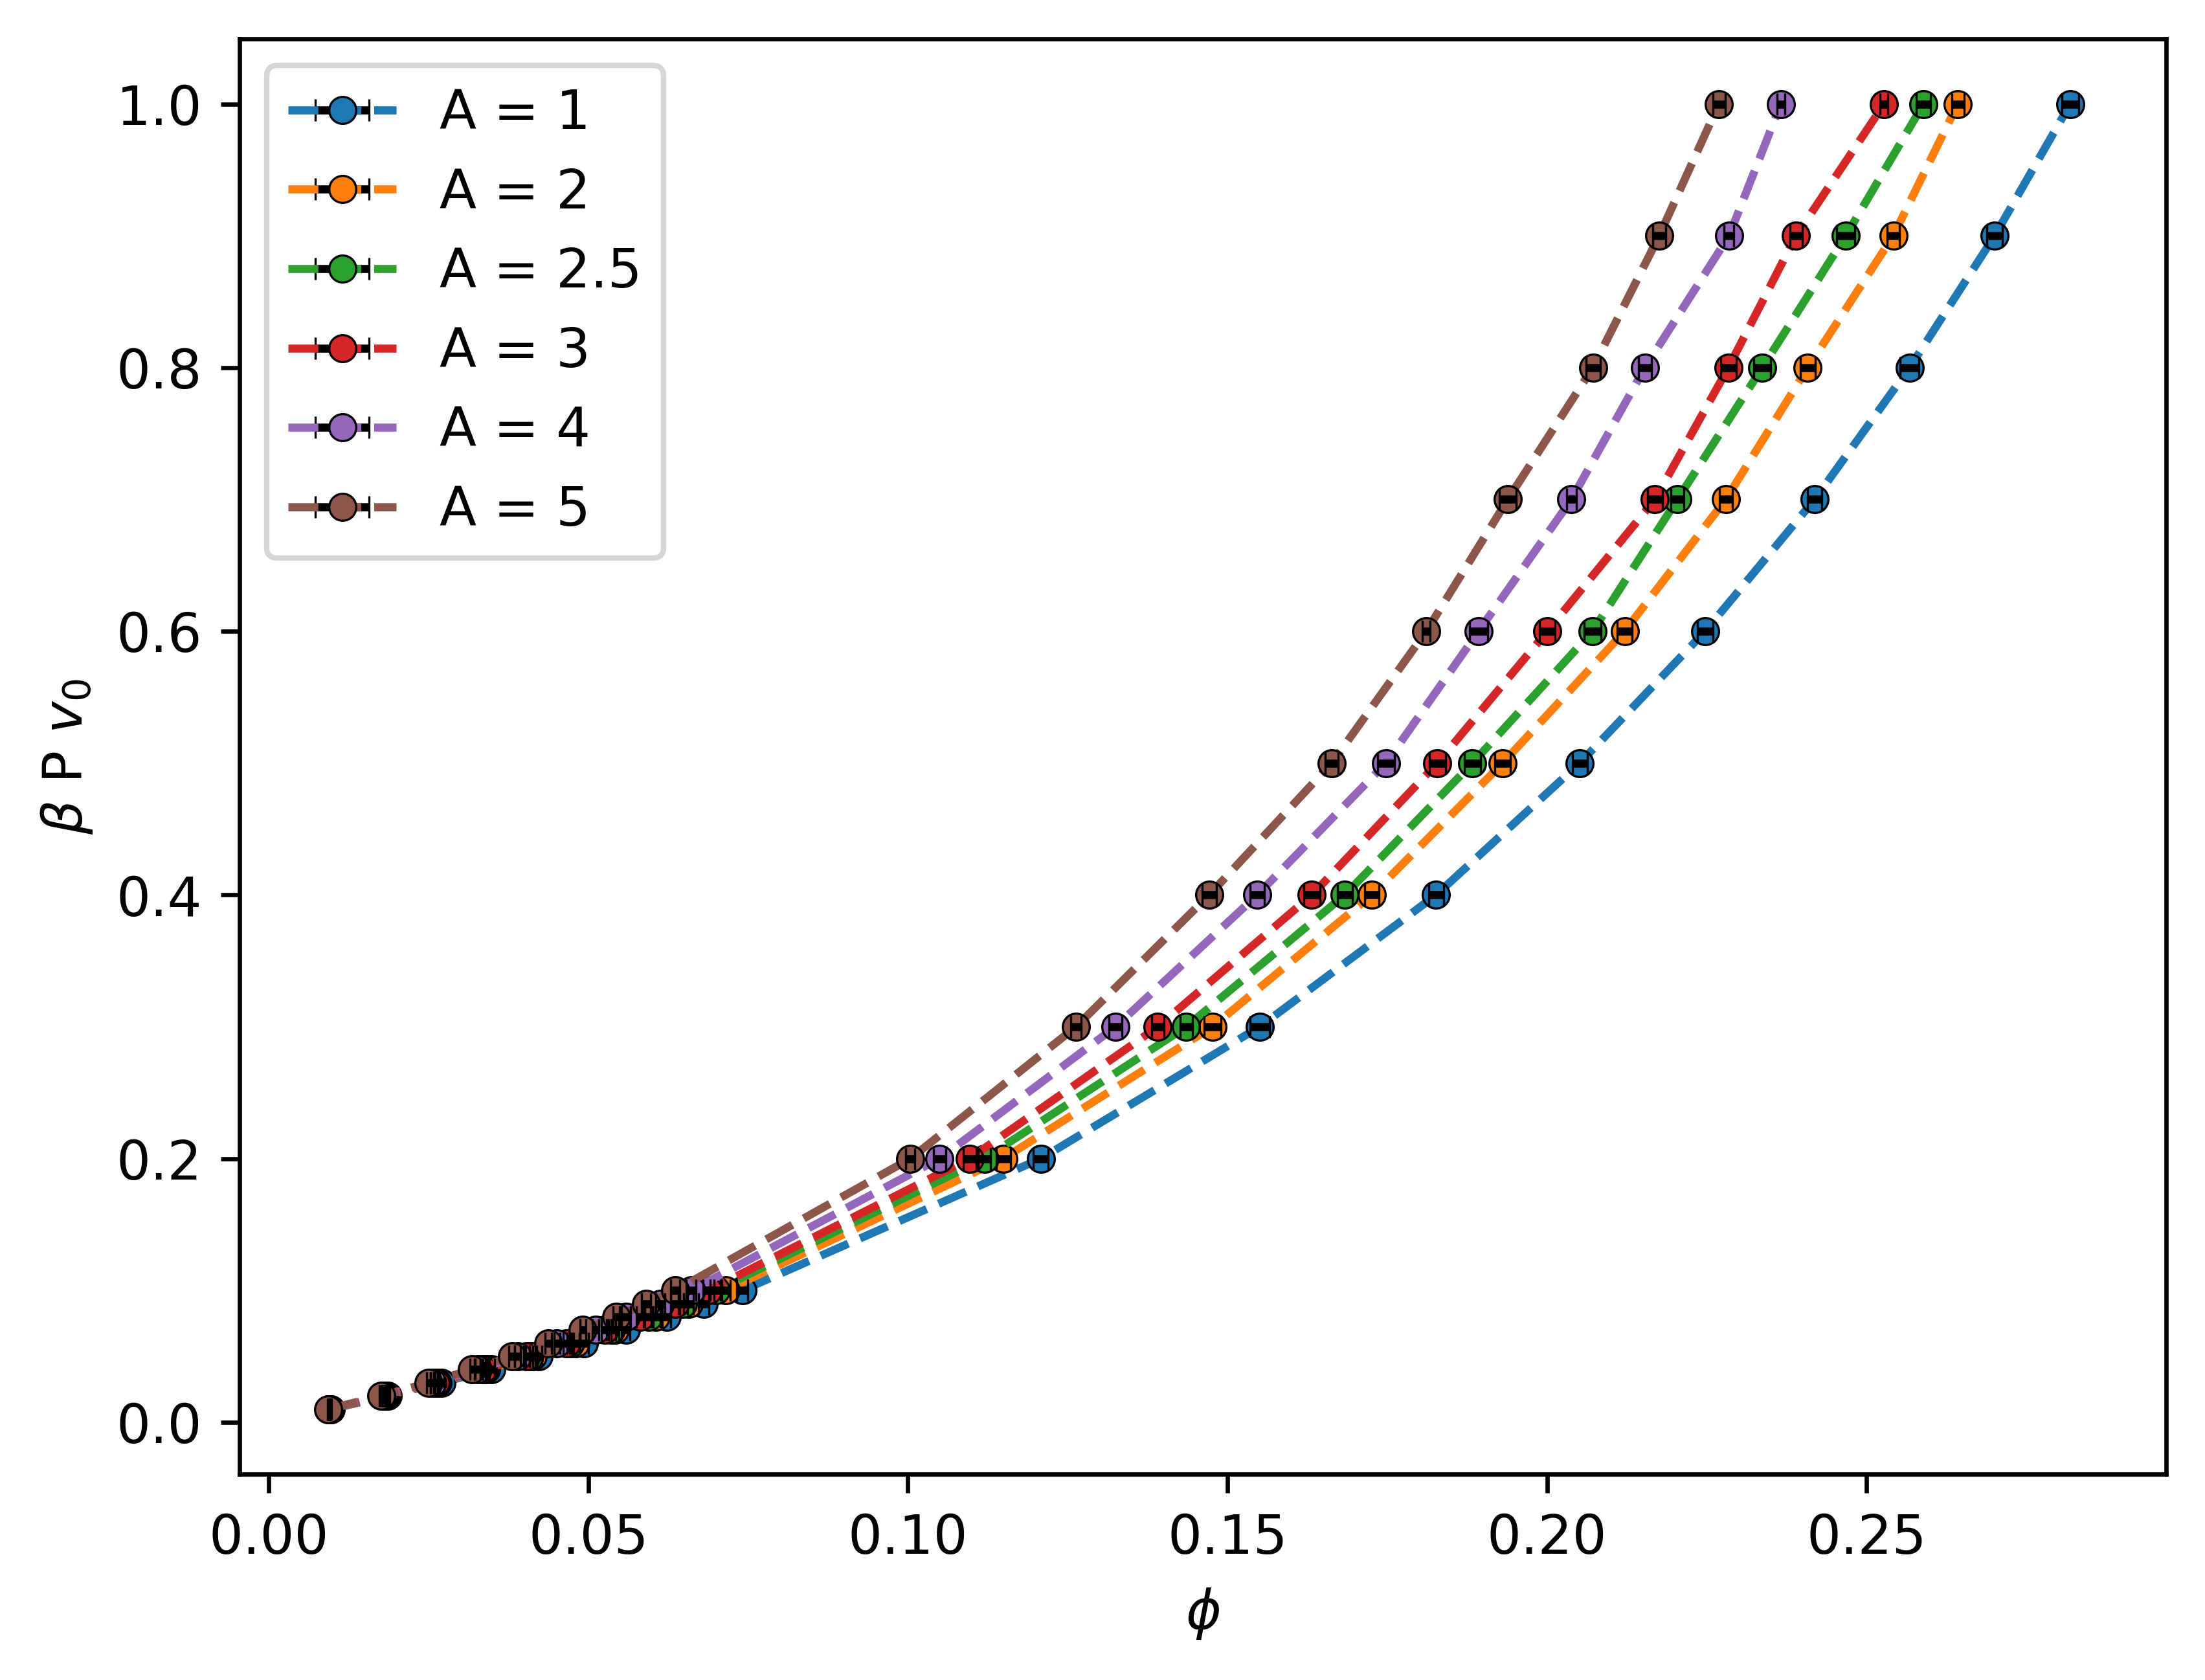
\includegraphics[width=0.3 \columnwidth]{Figures/EOS/PolyDLGauss0.75.png}
    \caption{Phase diagram of hard spherocylinders for different aspect ratios for all the cases analysed in this work. (METTERE I DATI E I MARKER GIUSTI, TOGLIERE LE LEGENDE, AUMENTARE I LABEL, AGGIUNGERE UN MODO PER DISTINGUERE I VARI CASI)}
    \label{fig:EOS_tot}
\end{figure}
%%%%%%%%%%%%%

\section{Nematic Order Parameter}
 We report in figure \ref{fig:S_par} the nematic order parameter $S$ for all the different systems analysed in this work. The values of $S$ are coherent with a isotropic phase for all the reduced pressures, all the aspect ratios and polydispersities.

\begin{figure}[!h]
    \centering
    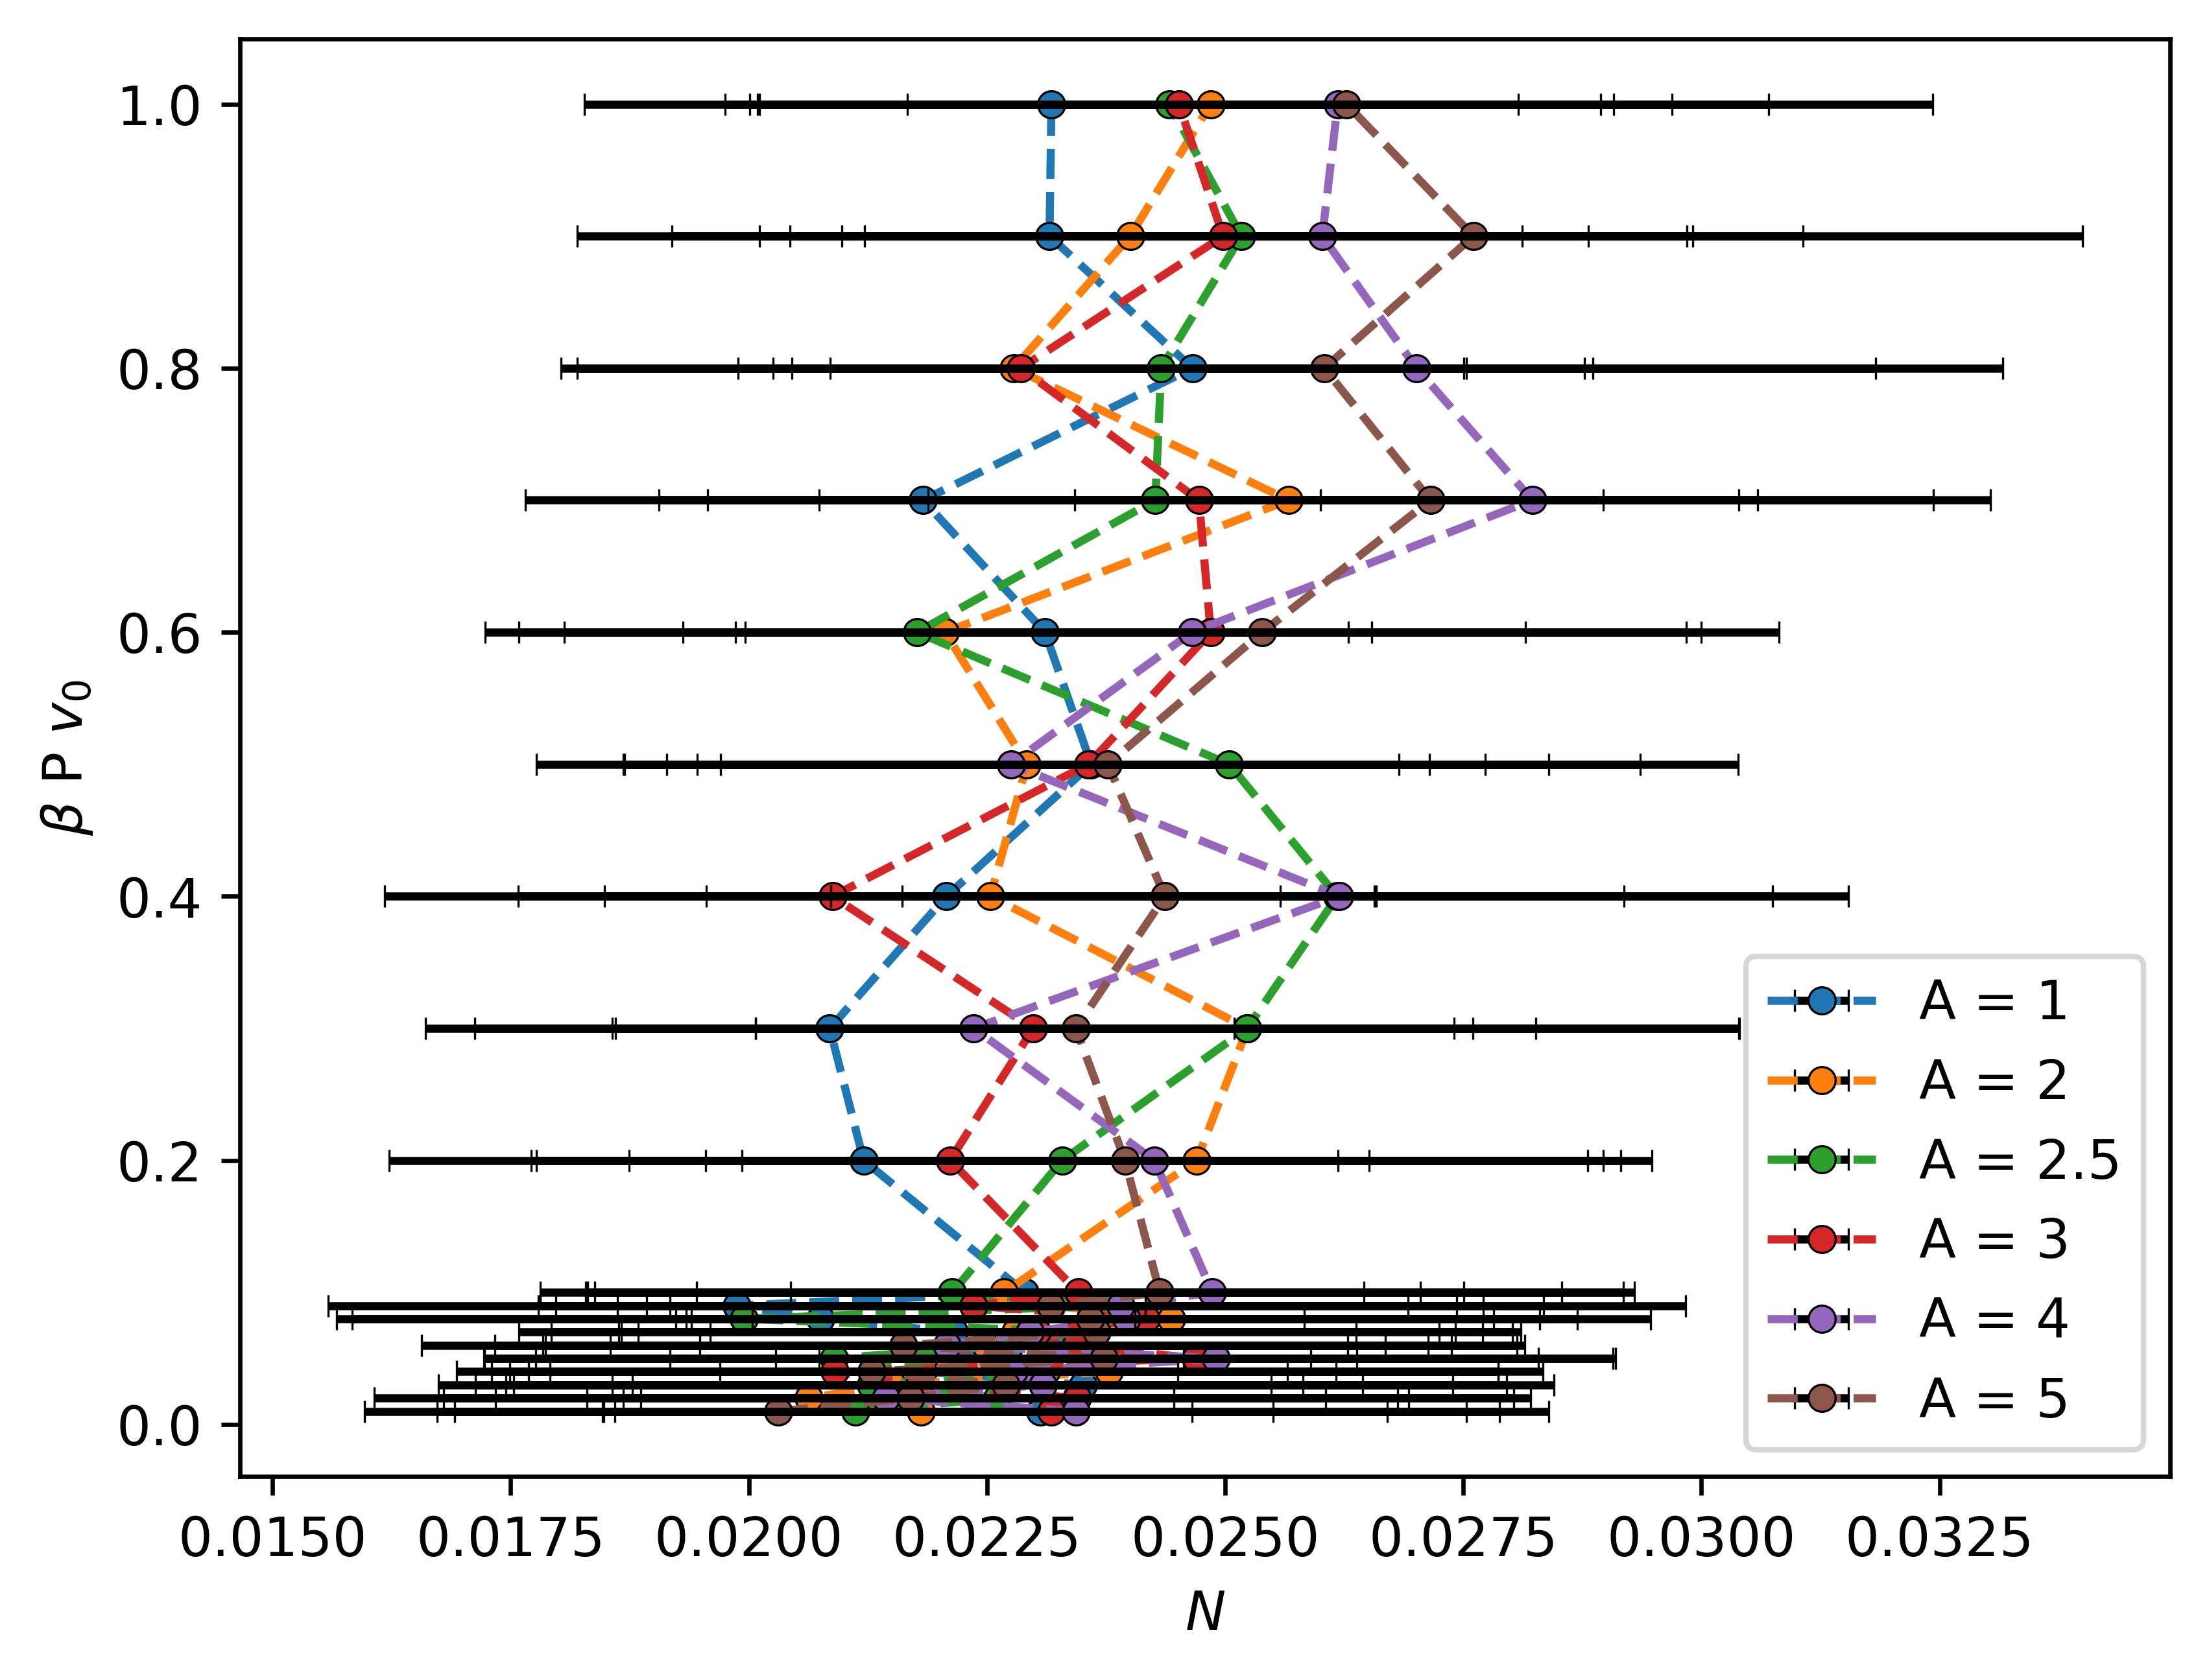
\includegraphics[width=0.3 \columnwidth]{Figures/S/Mono.png}
    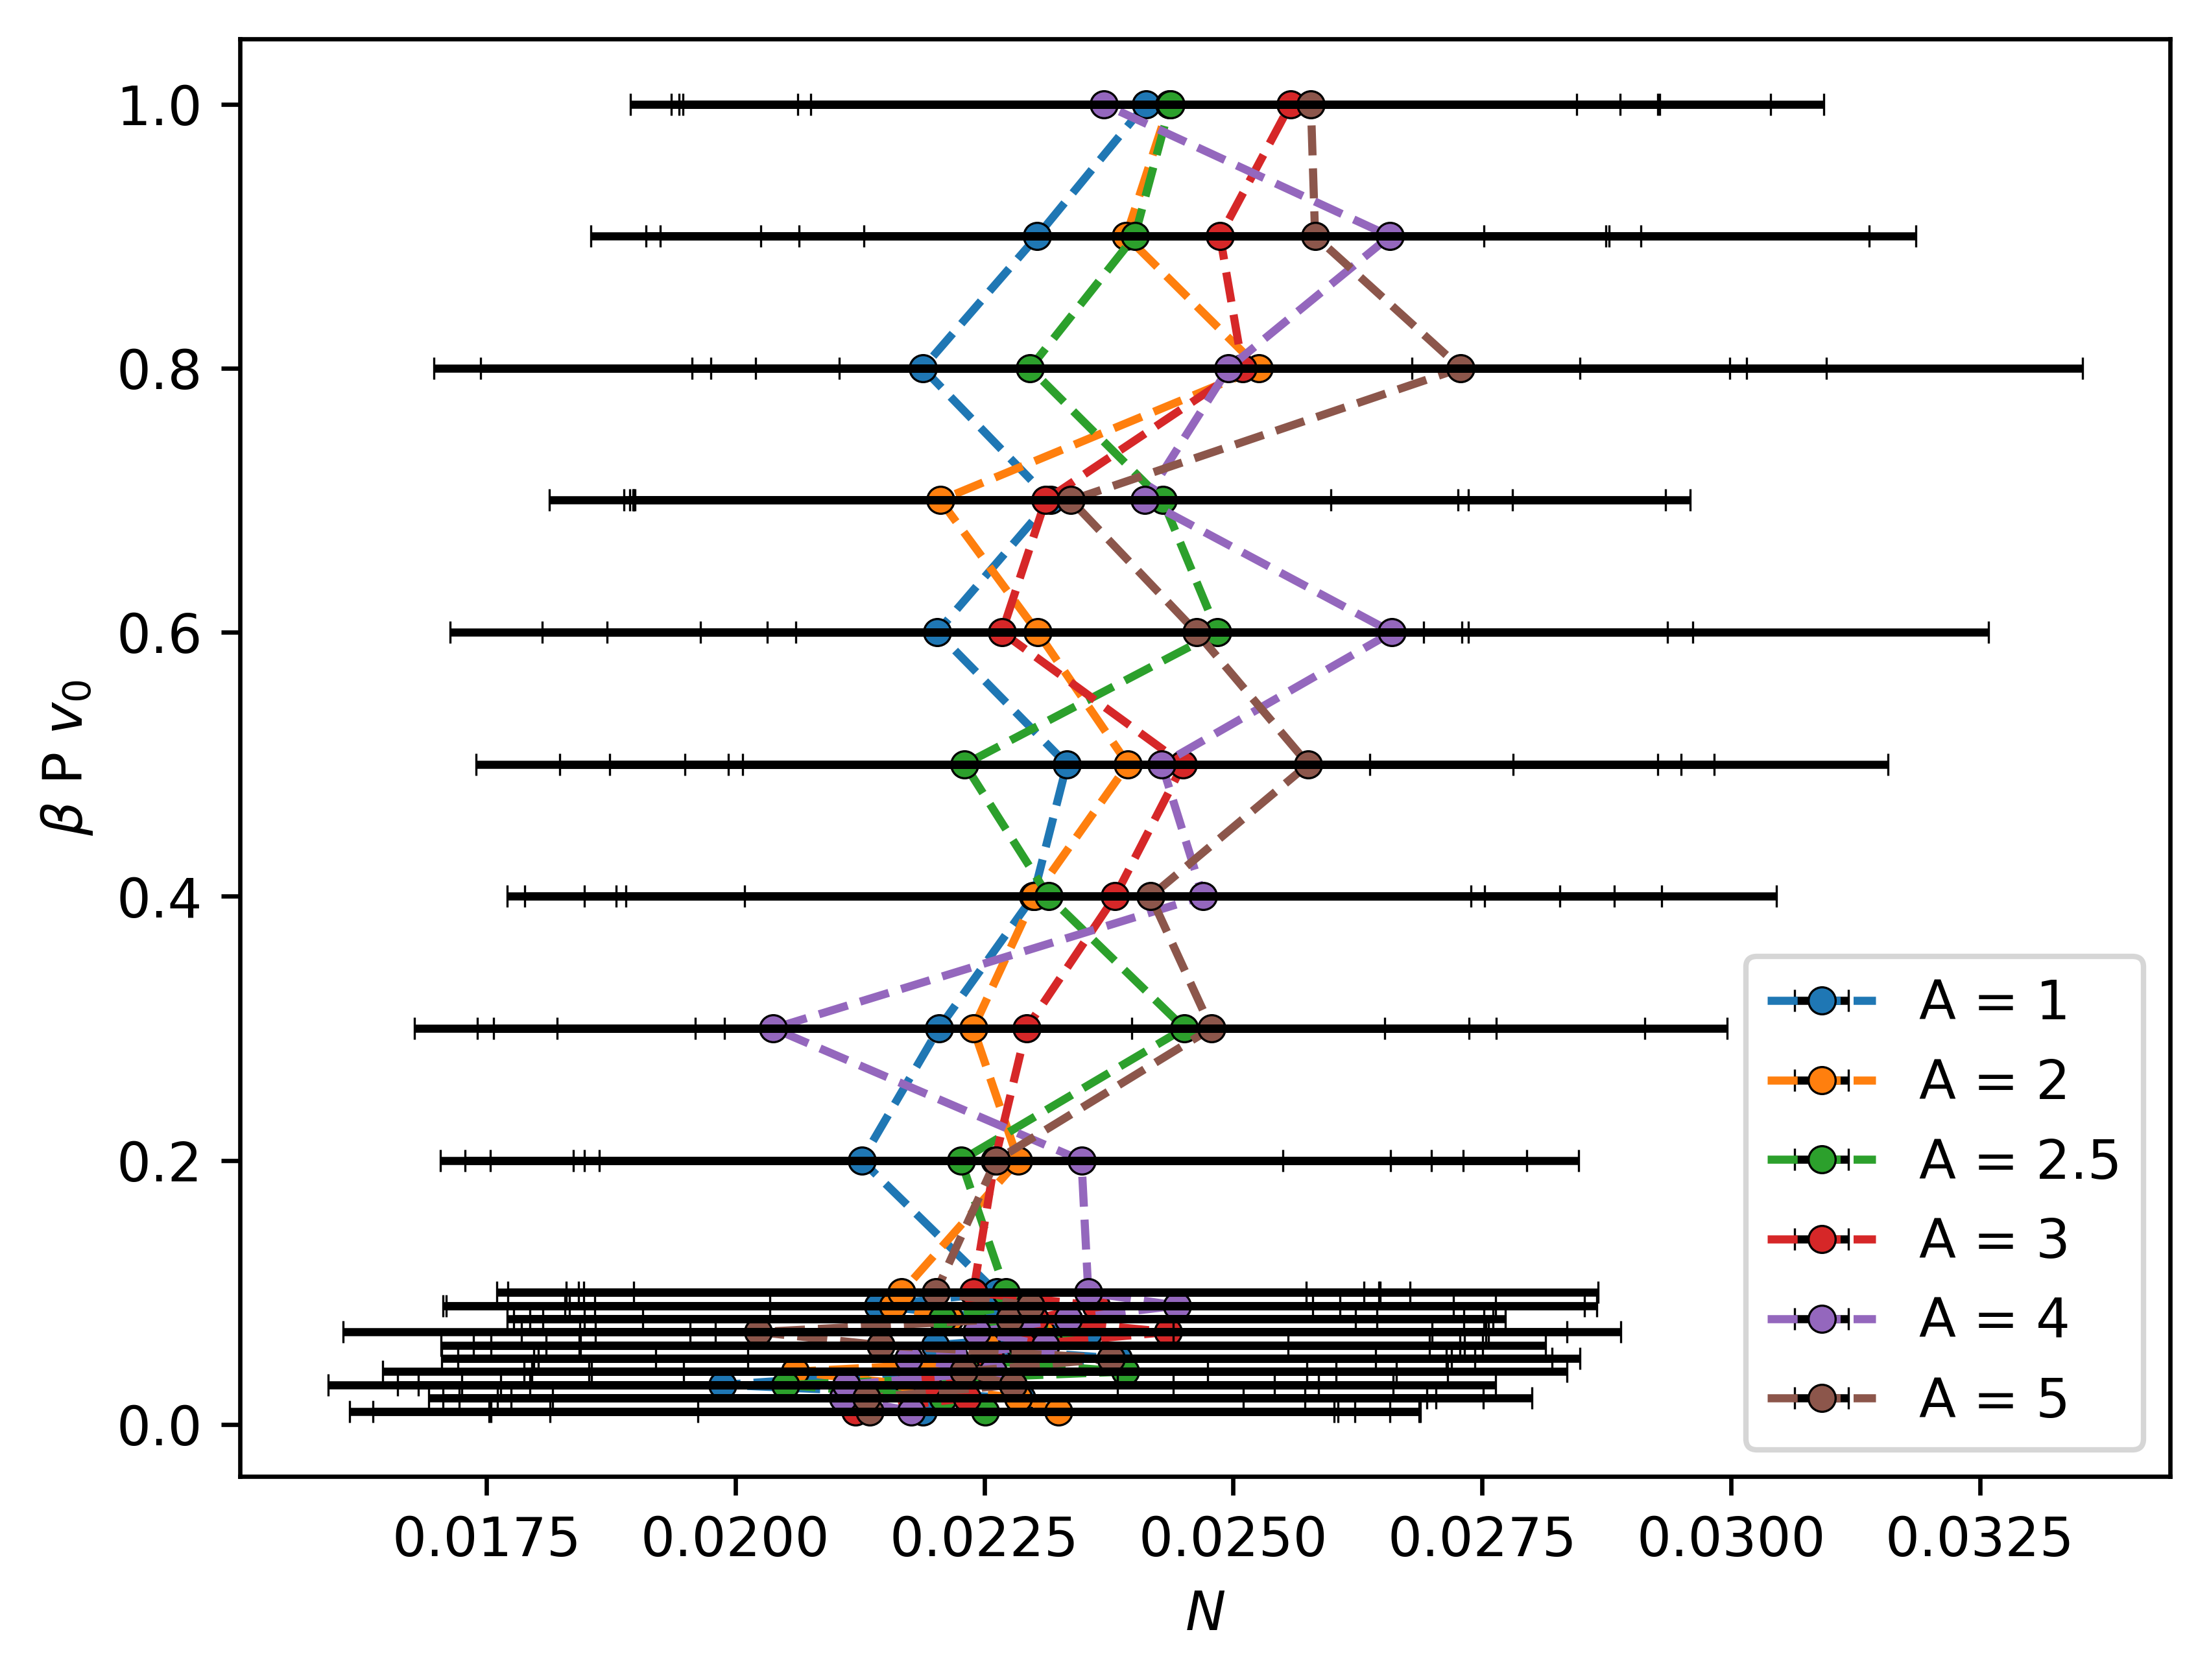
\includegraphics[width=0.3 \columnwidth]{Figures/S/PolyD.png}
    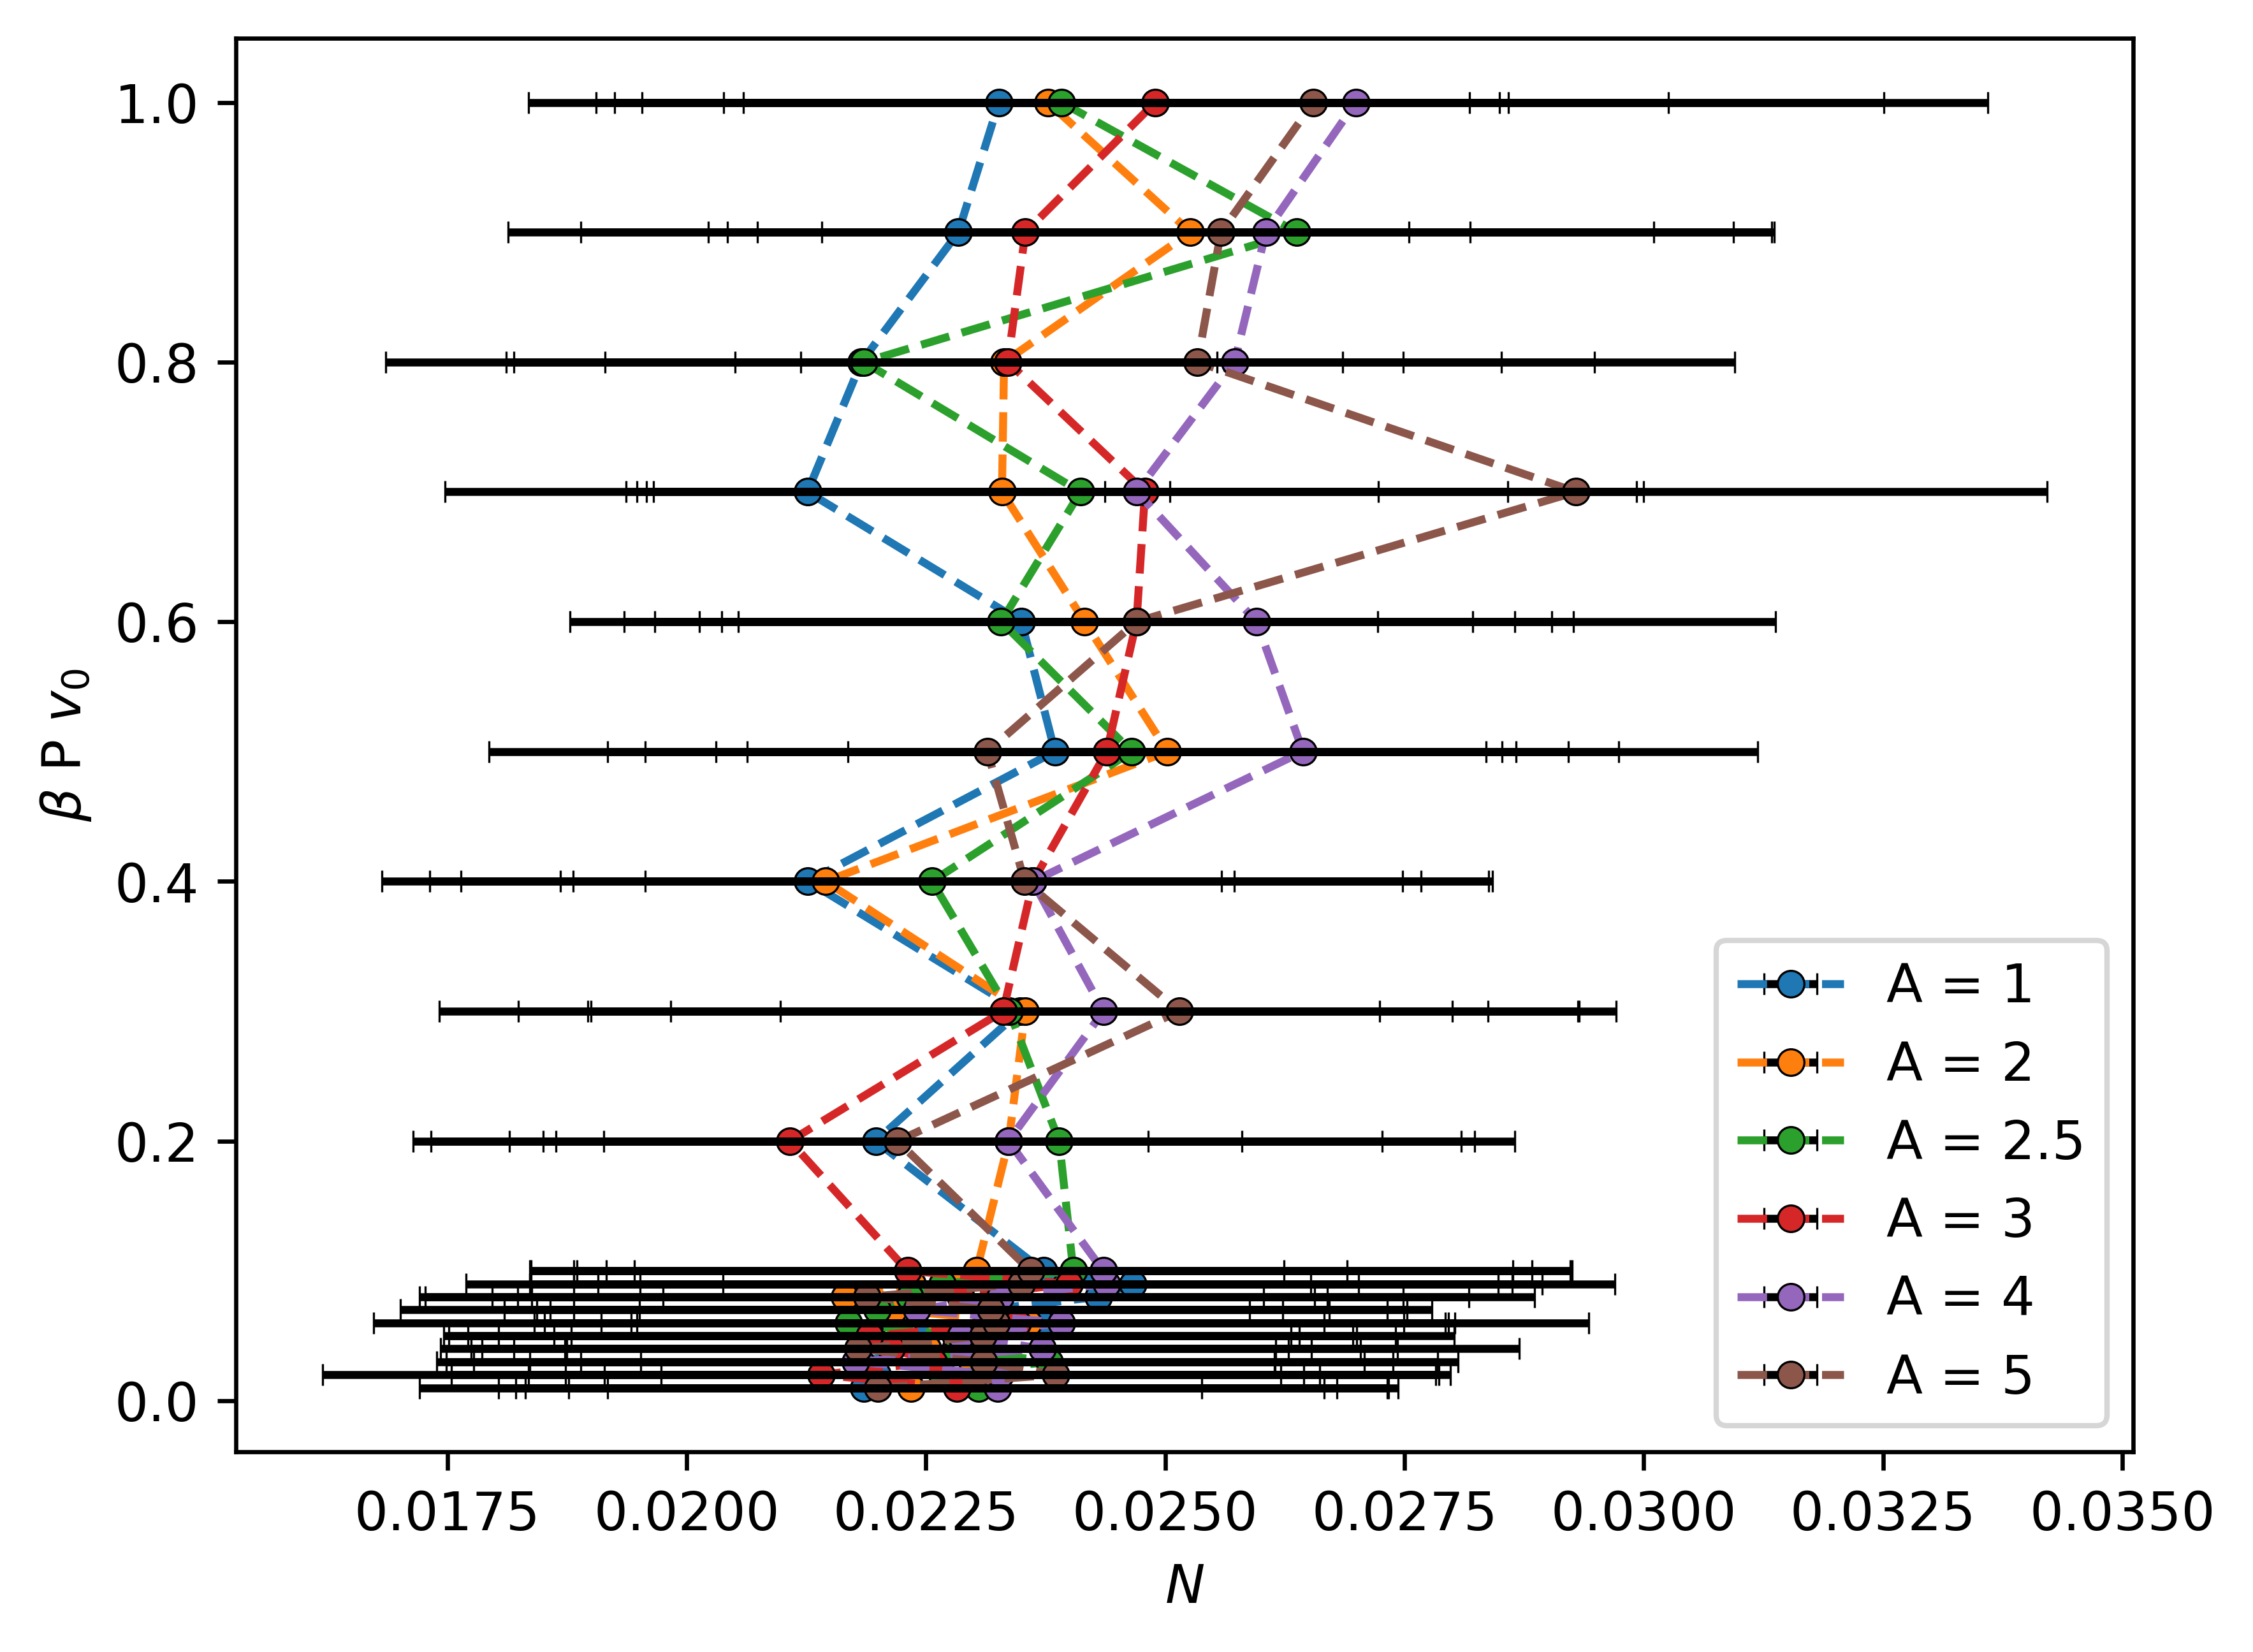
\includegraphics[width=0.3 \columnwidth]{Figures/S/PolyL.png}
    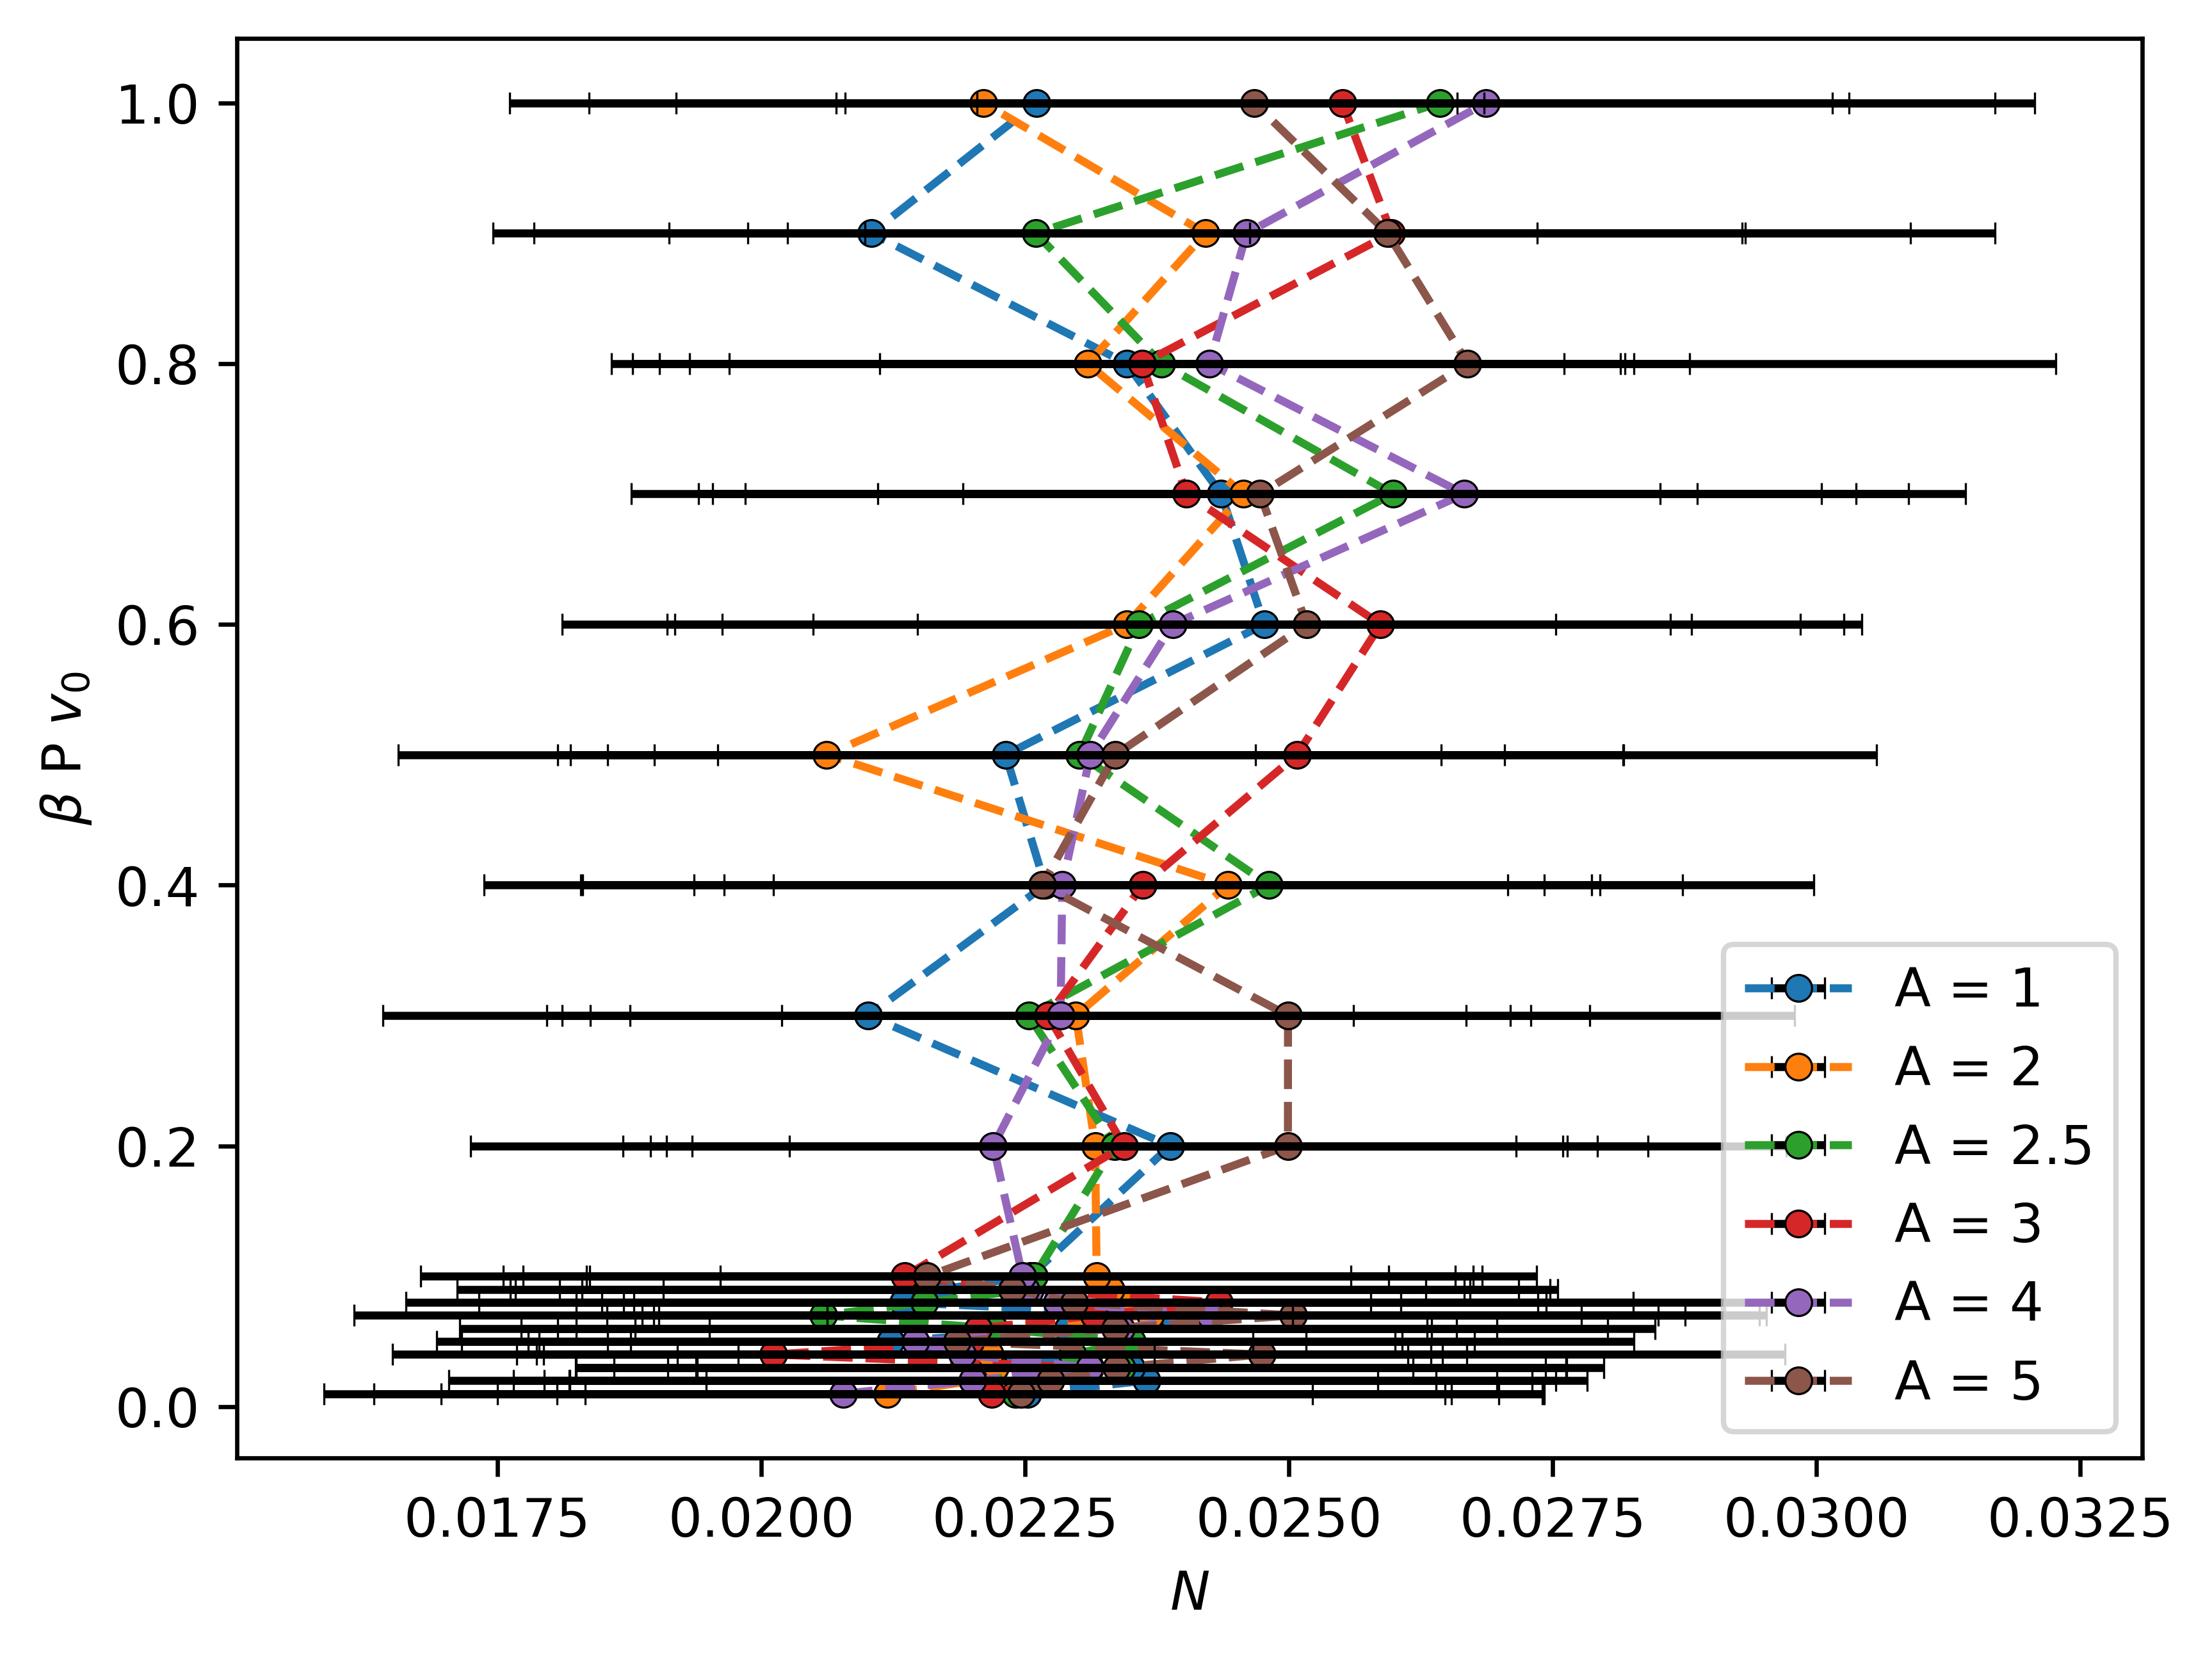
\includegraphics[width=0.3 \columnwidth]{Figures/S/PolyDGauss.png}
    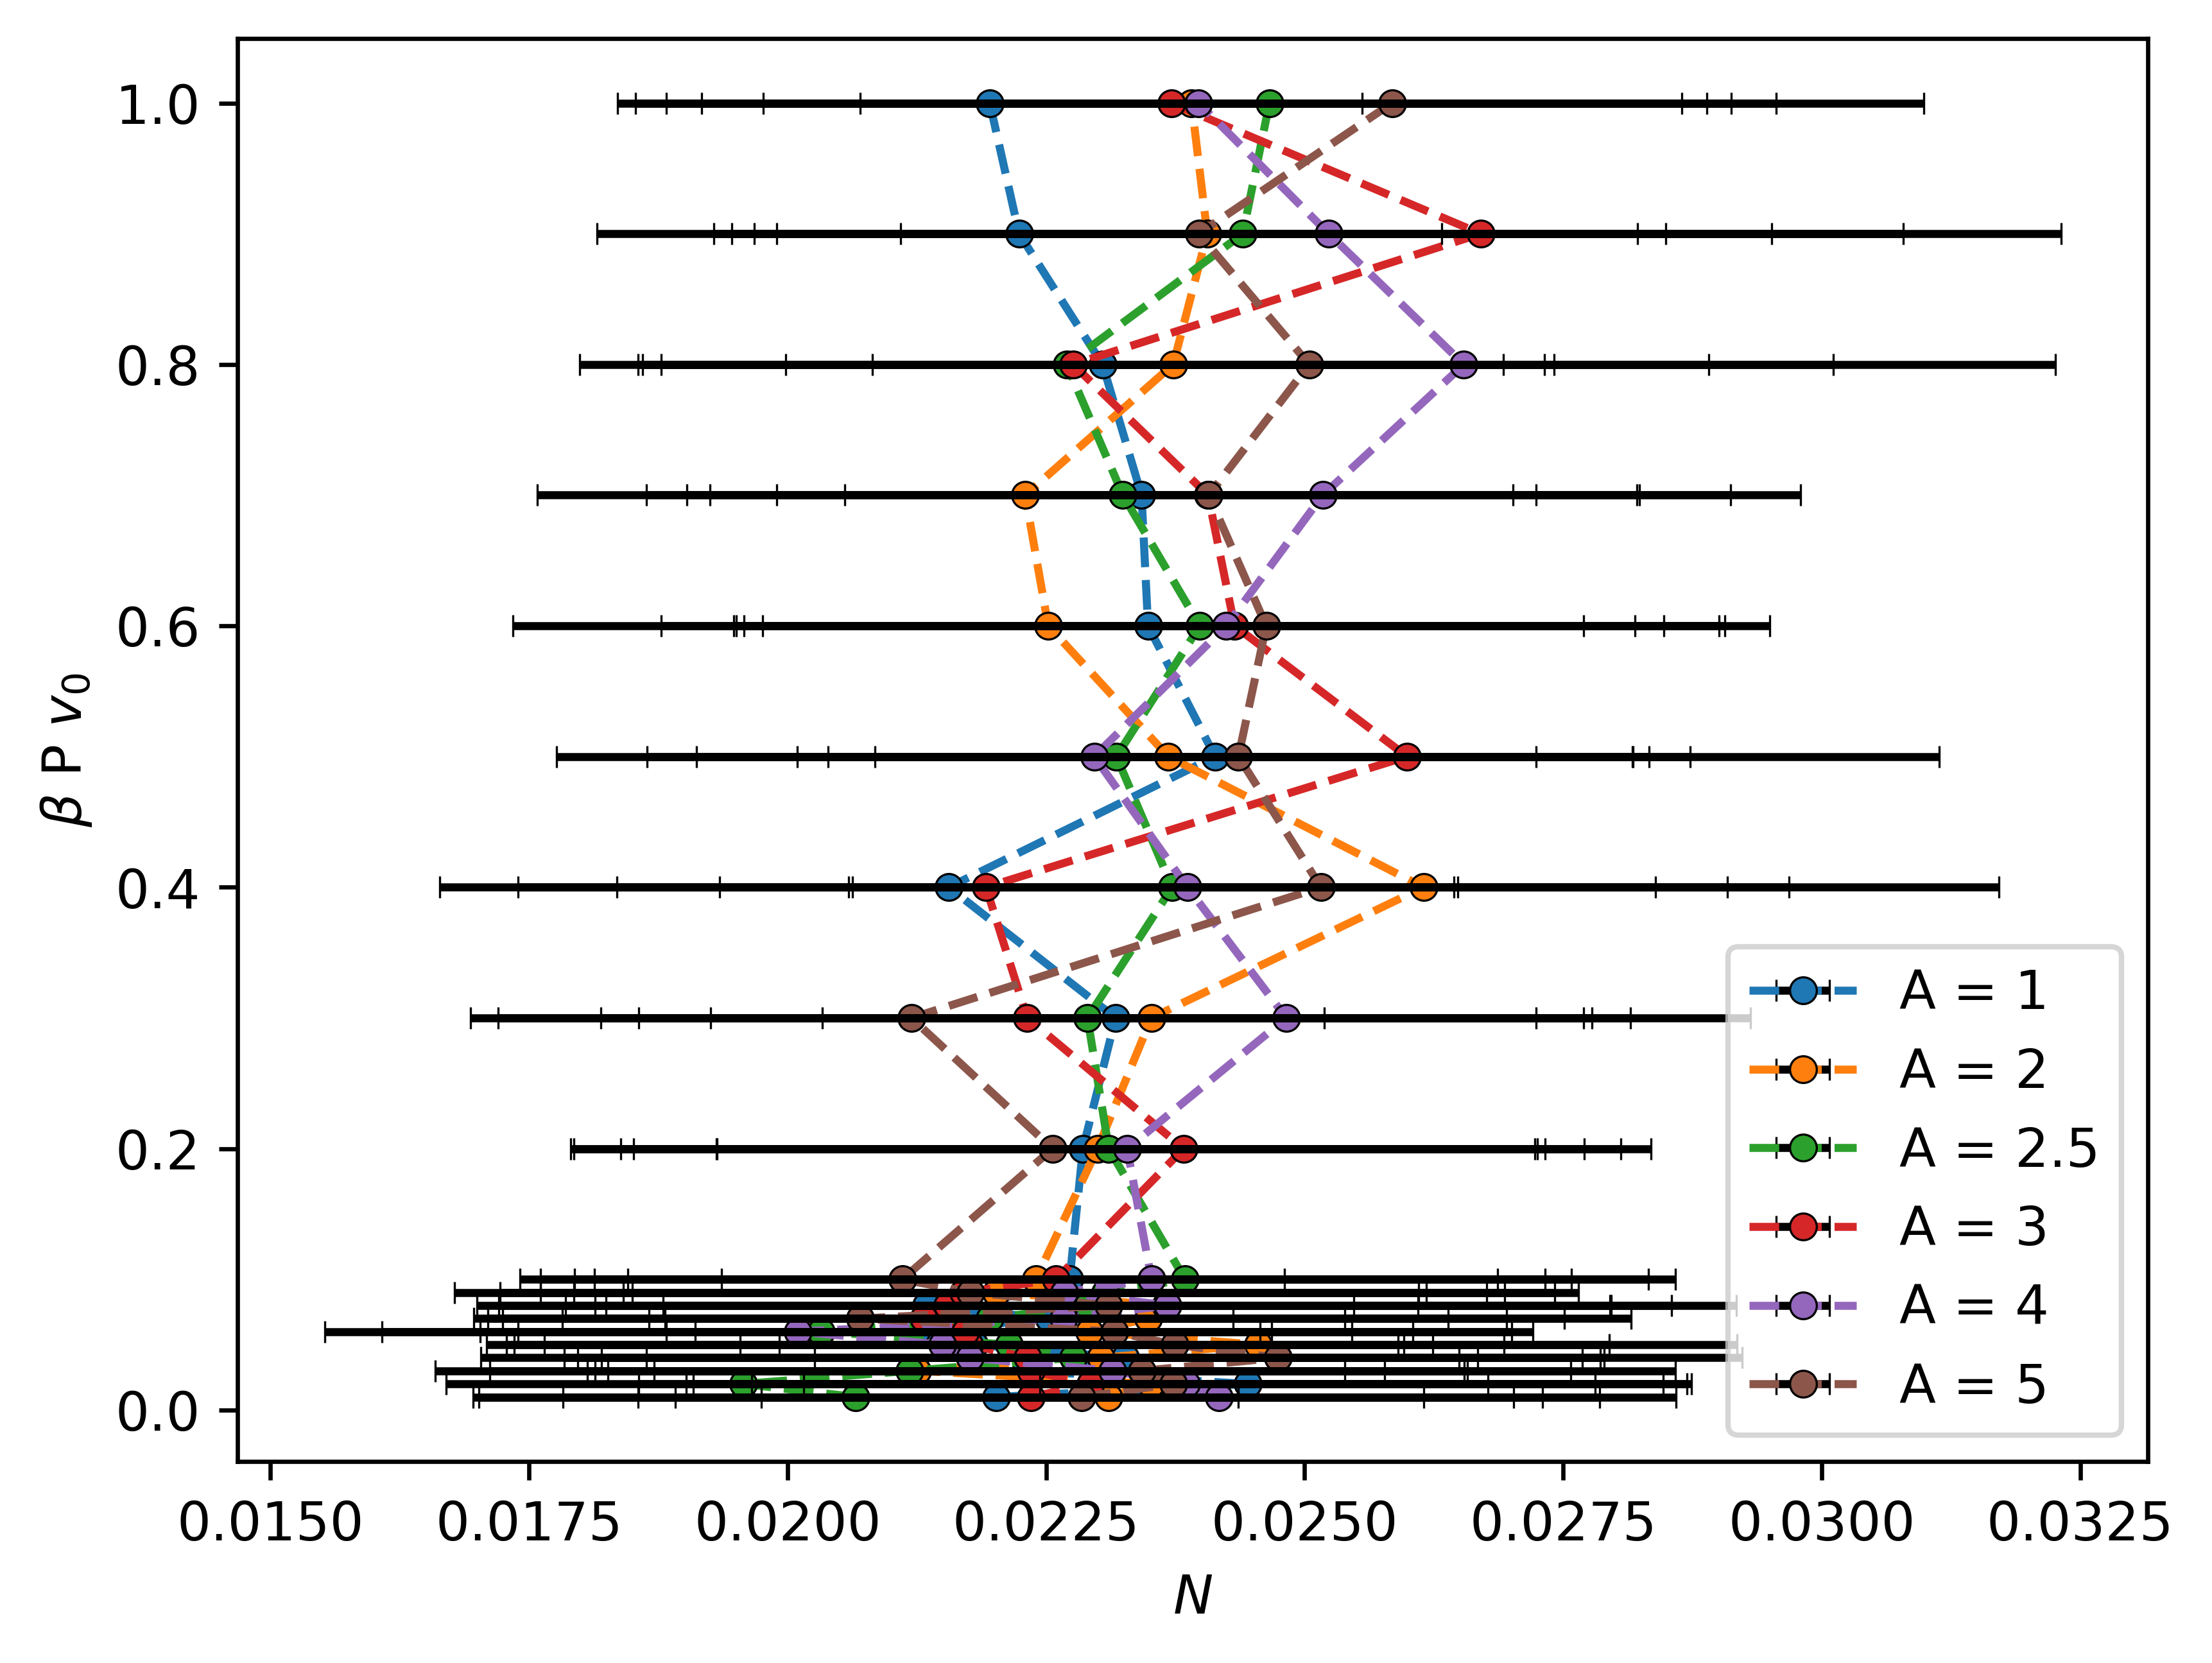
\includegraphics[width=0.3 \columnwidth]{Figures/S/PolyDLGauss.png}
    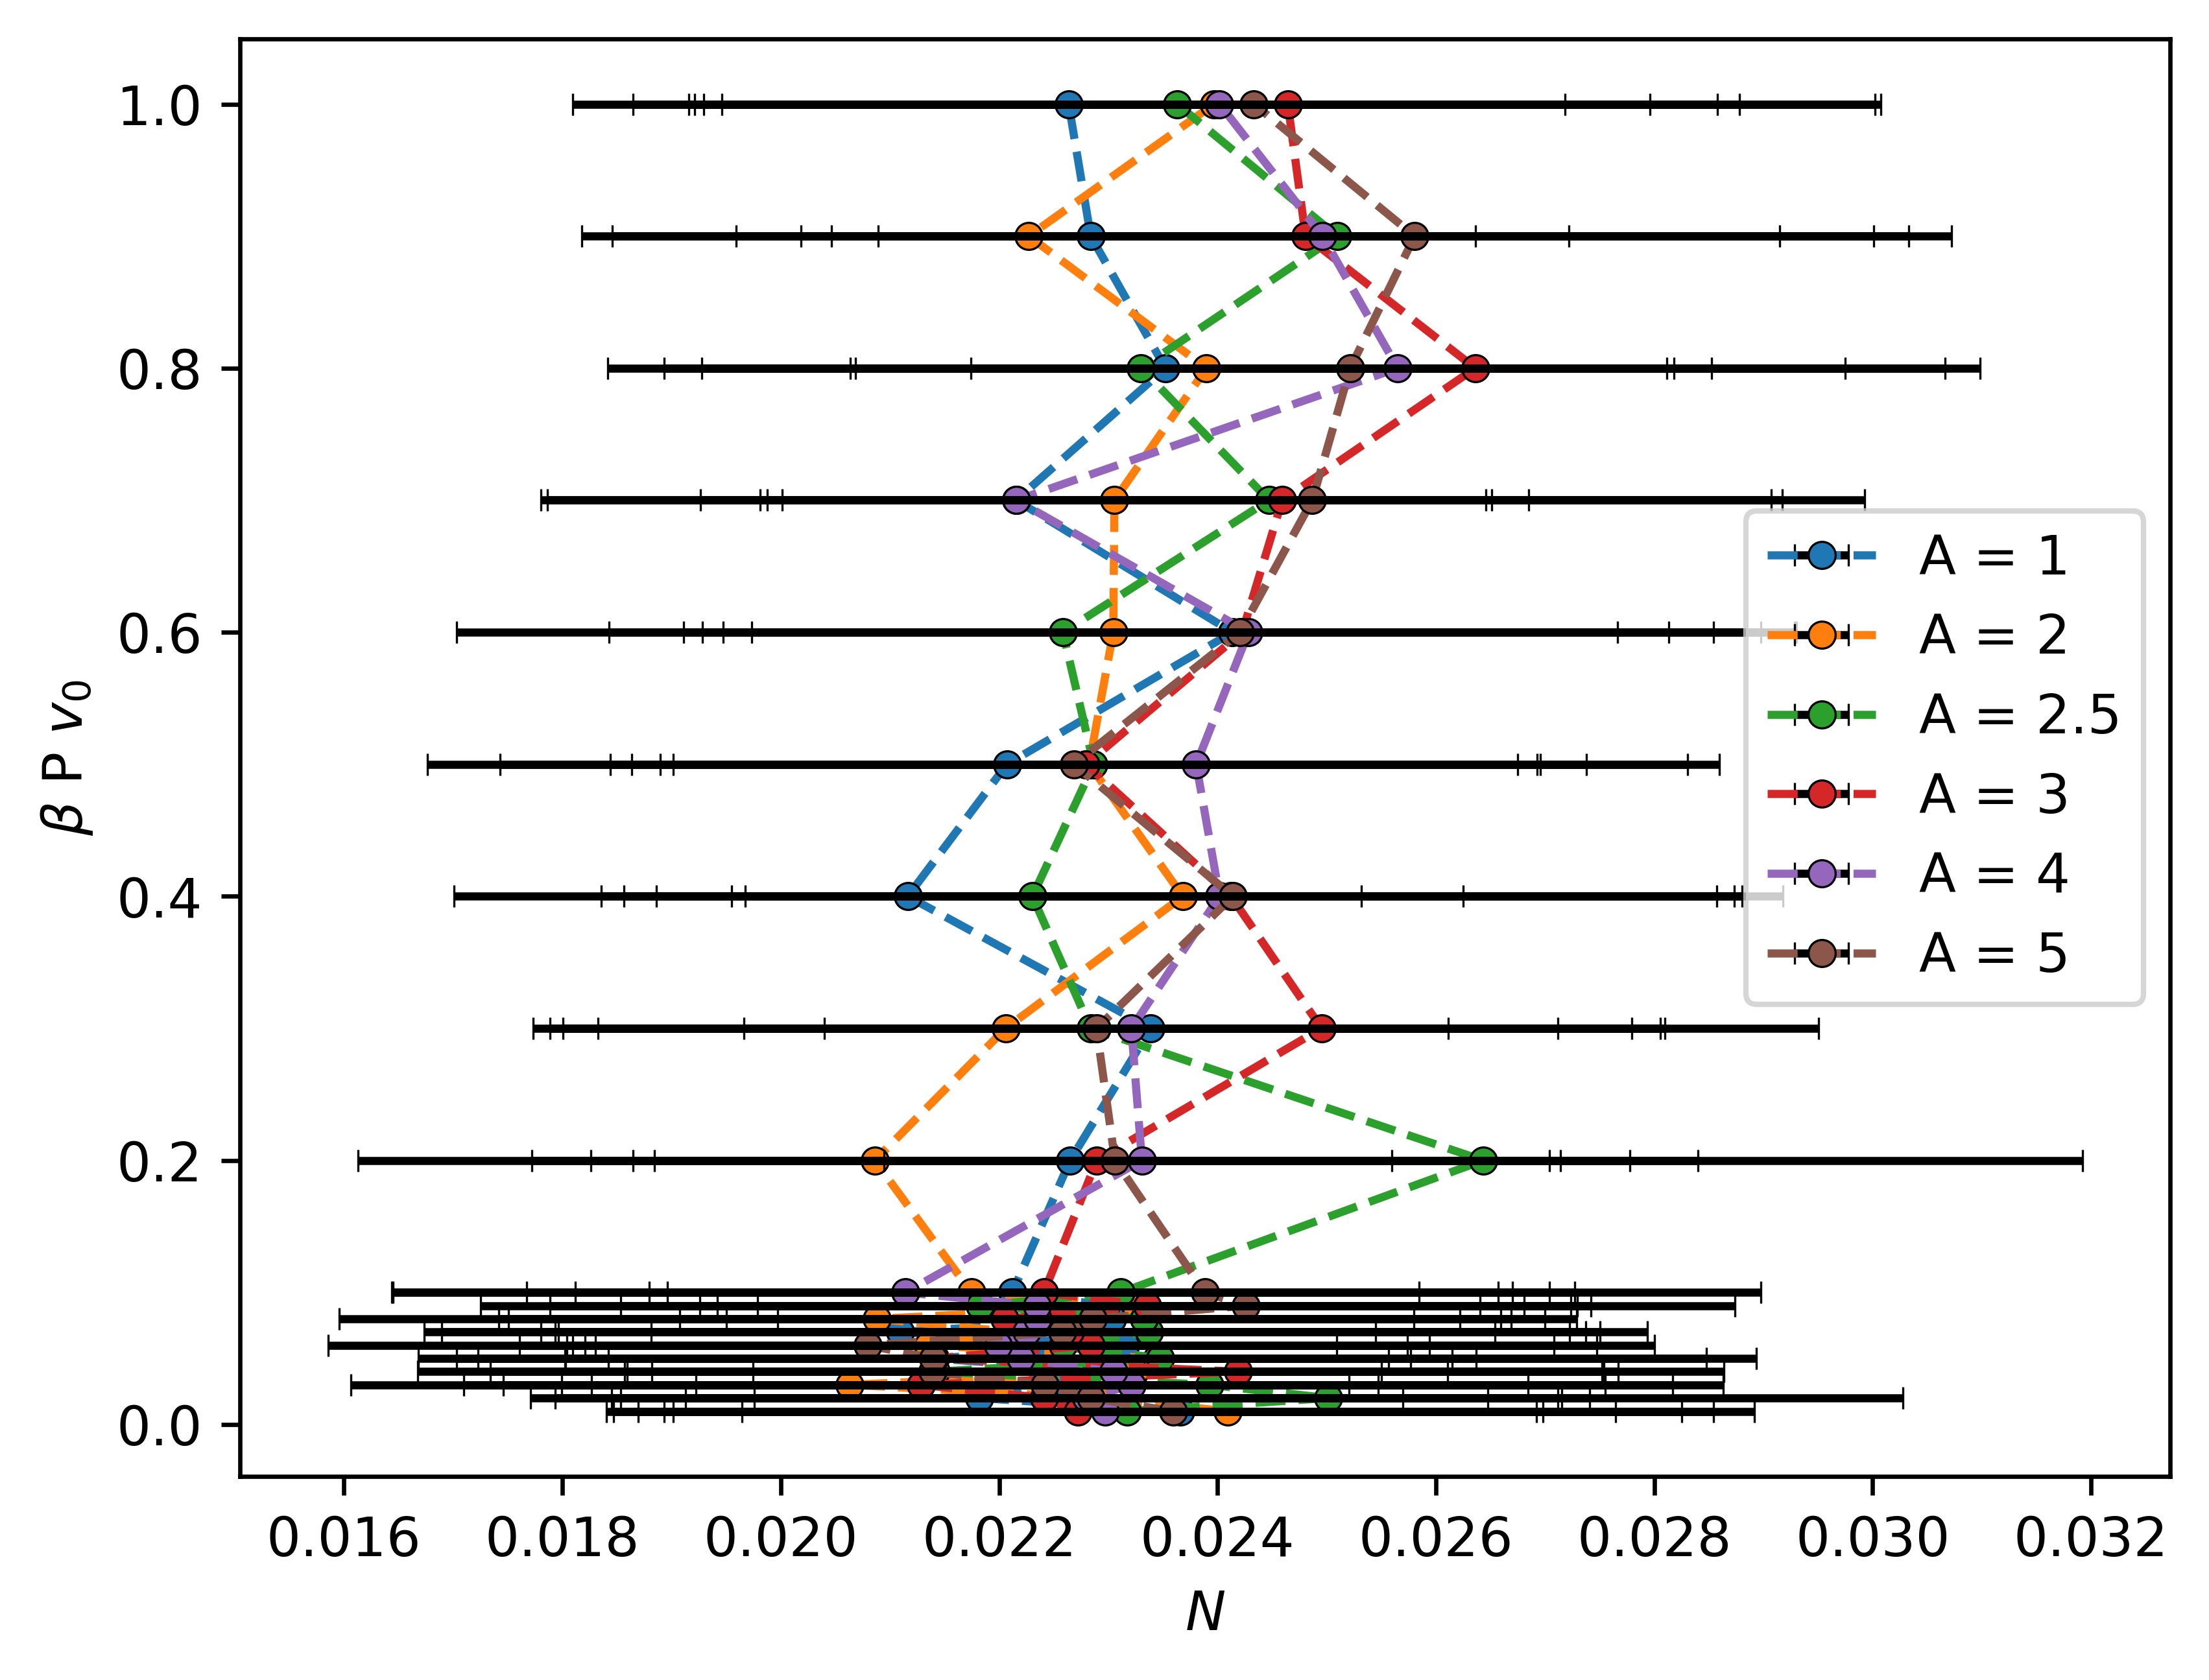
\includegraphics[width=0.3 \columnwidth]{Figures/S/PolyD0.75.png}
    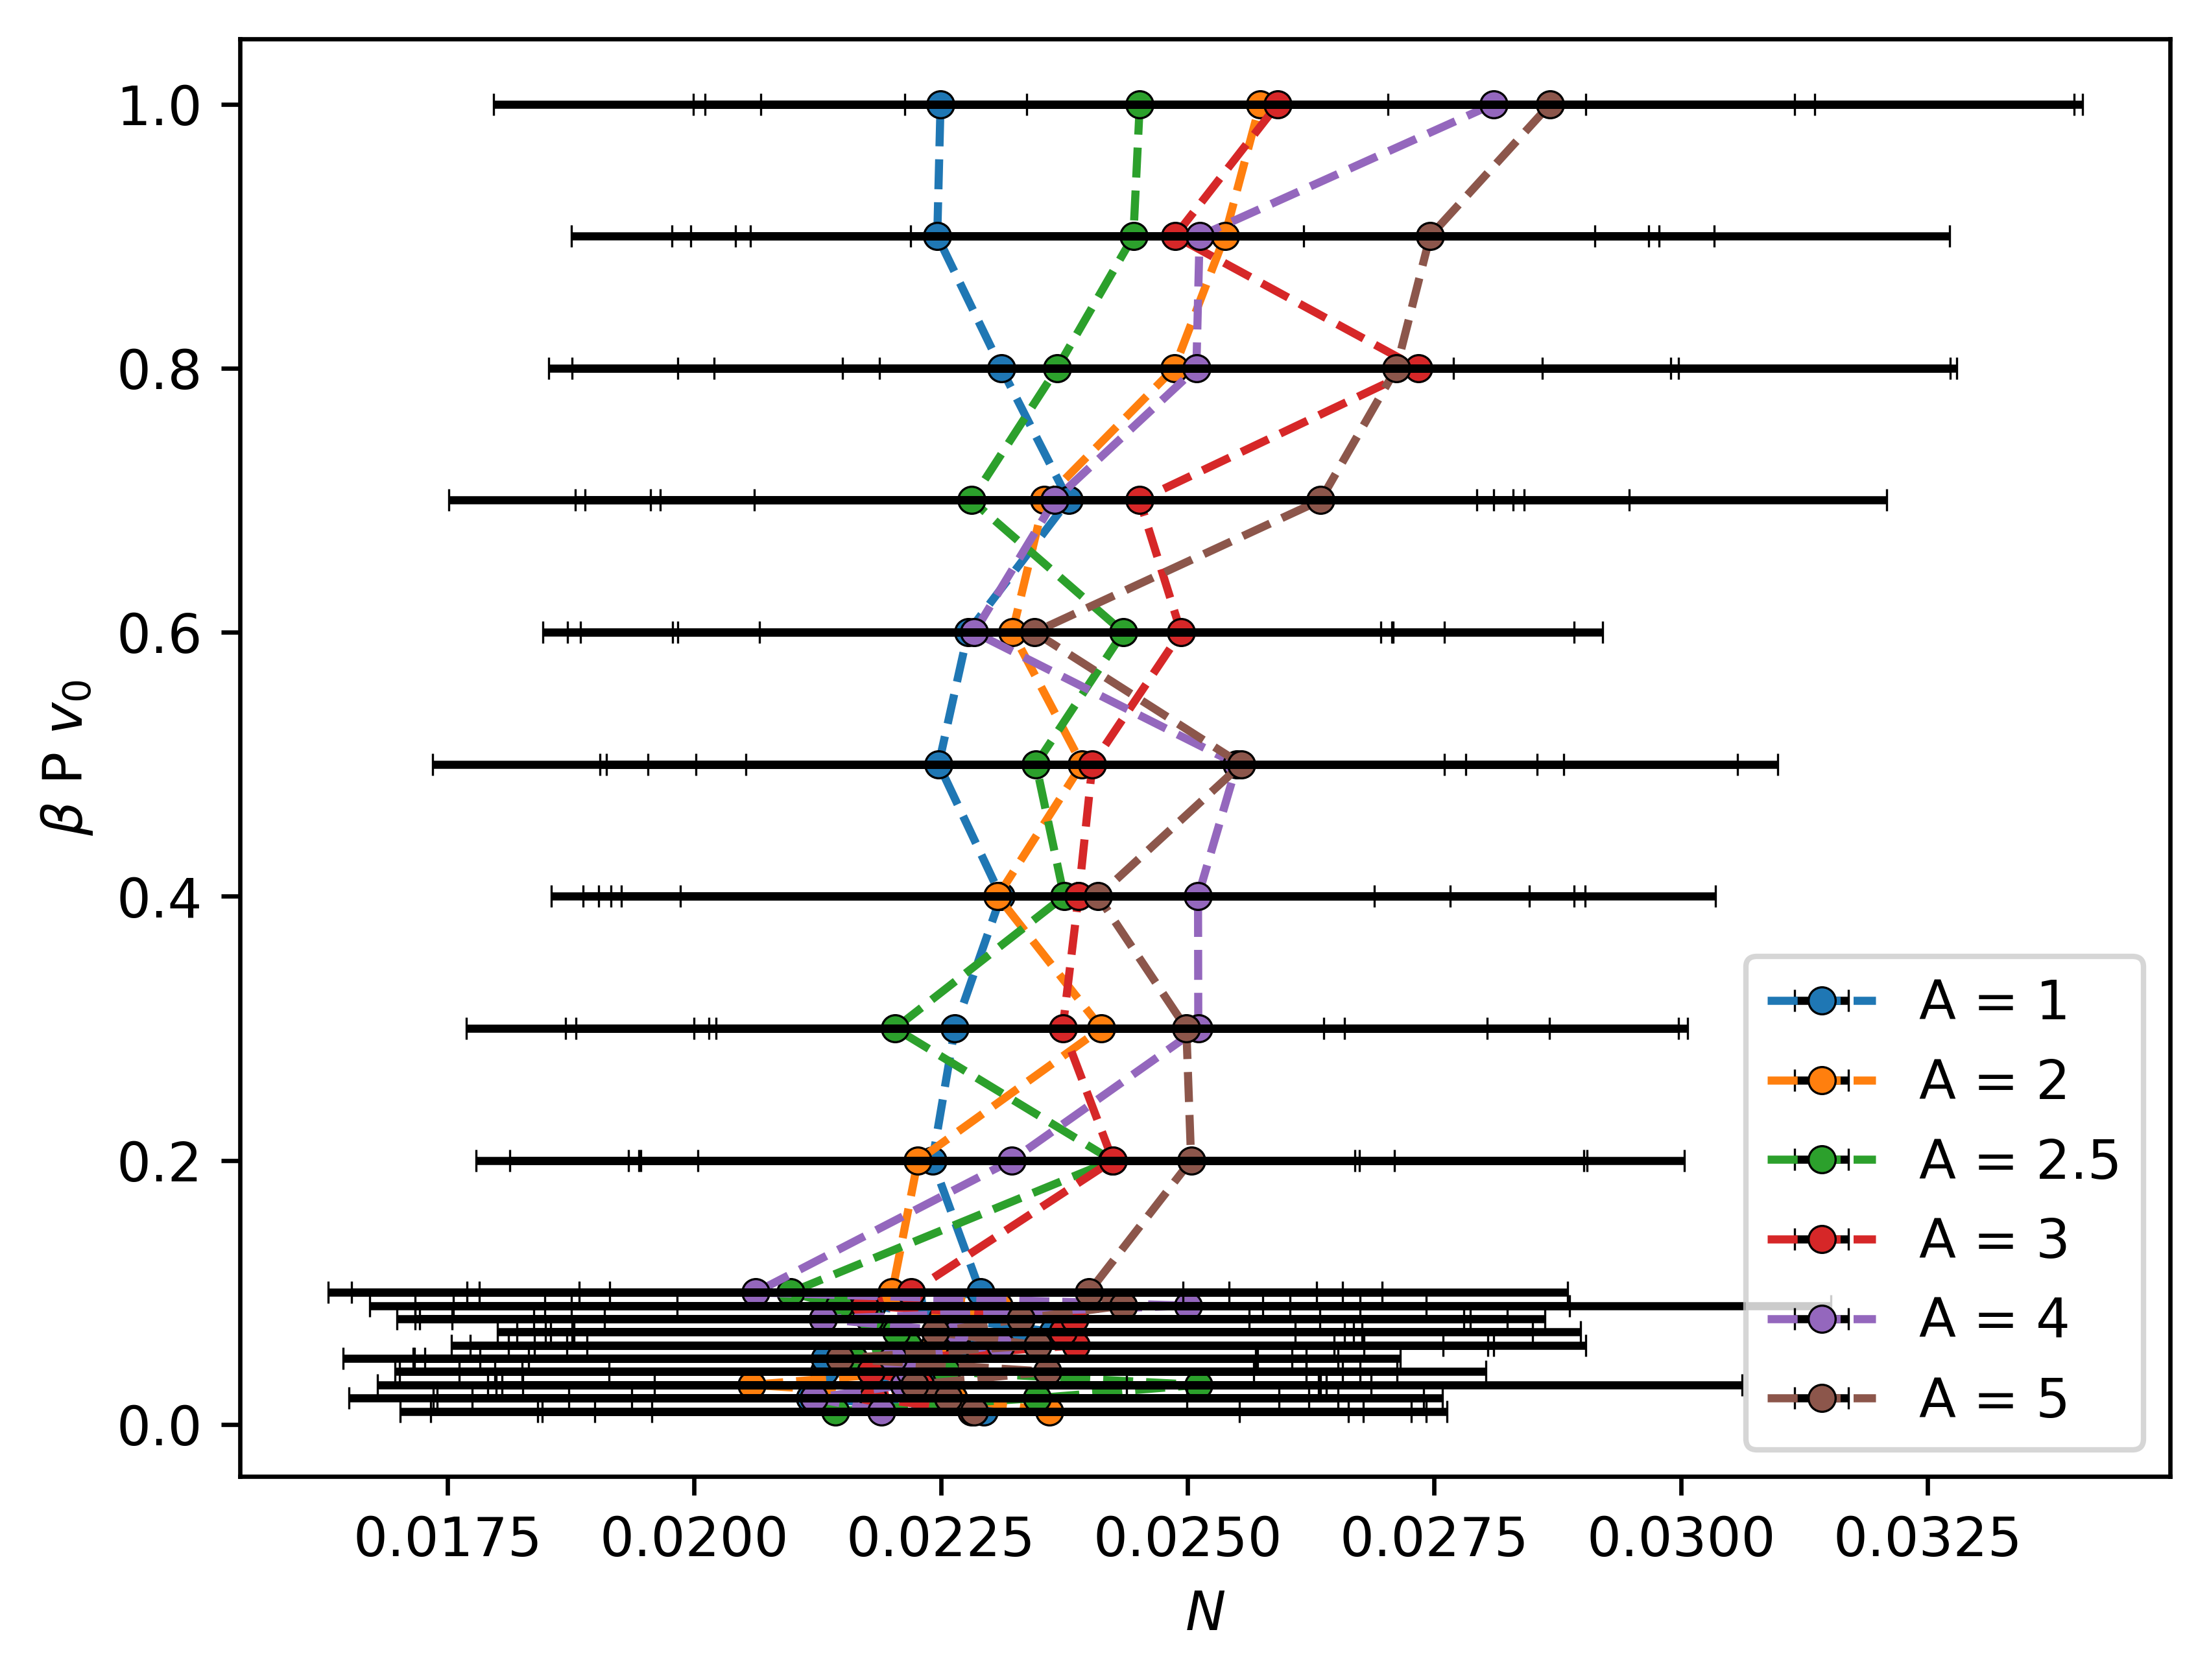
\includegraphics[width=0.3 \columnwidth]{Figures/S/PolyL0.75}
    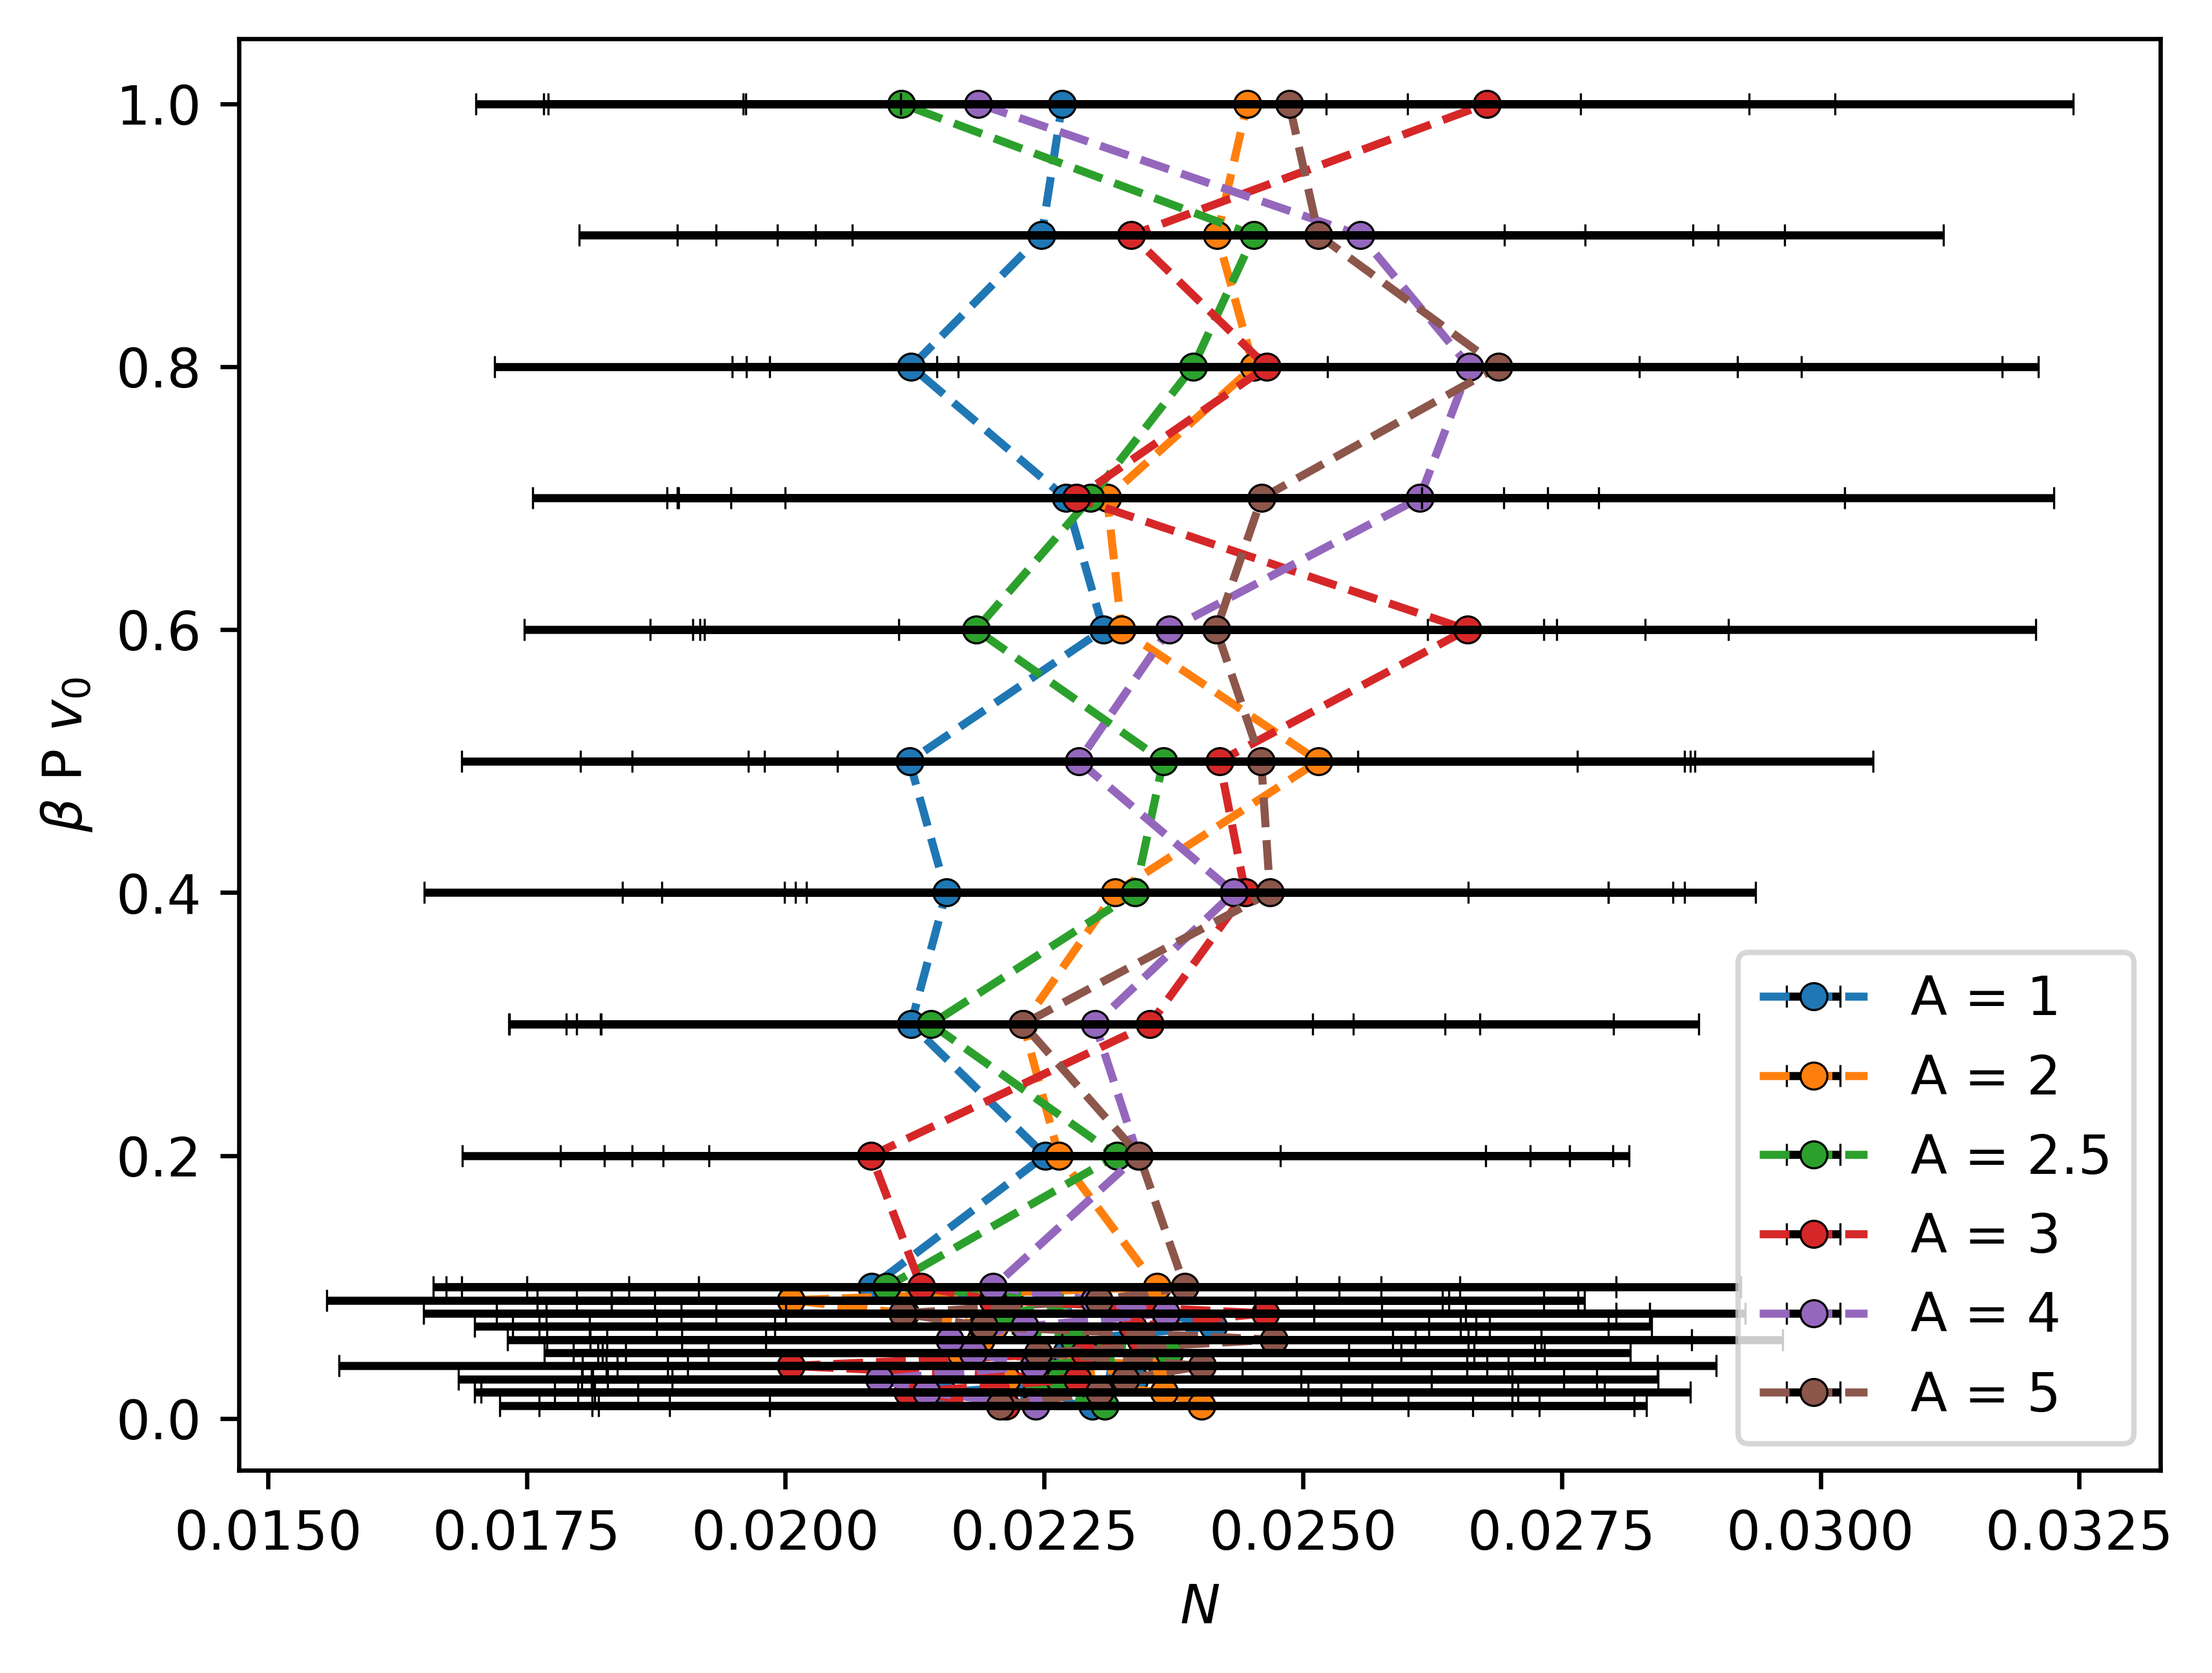
\includegraphics[width=0.3 \columnwidth]{Figures/S/PolyDGauss0.75.png}
    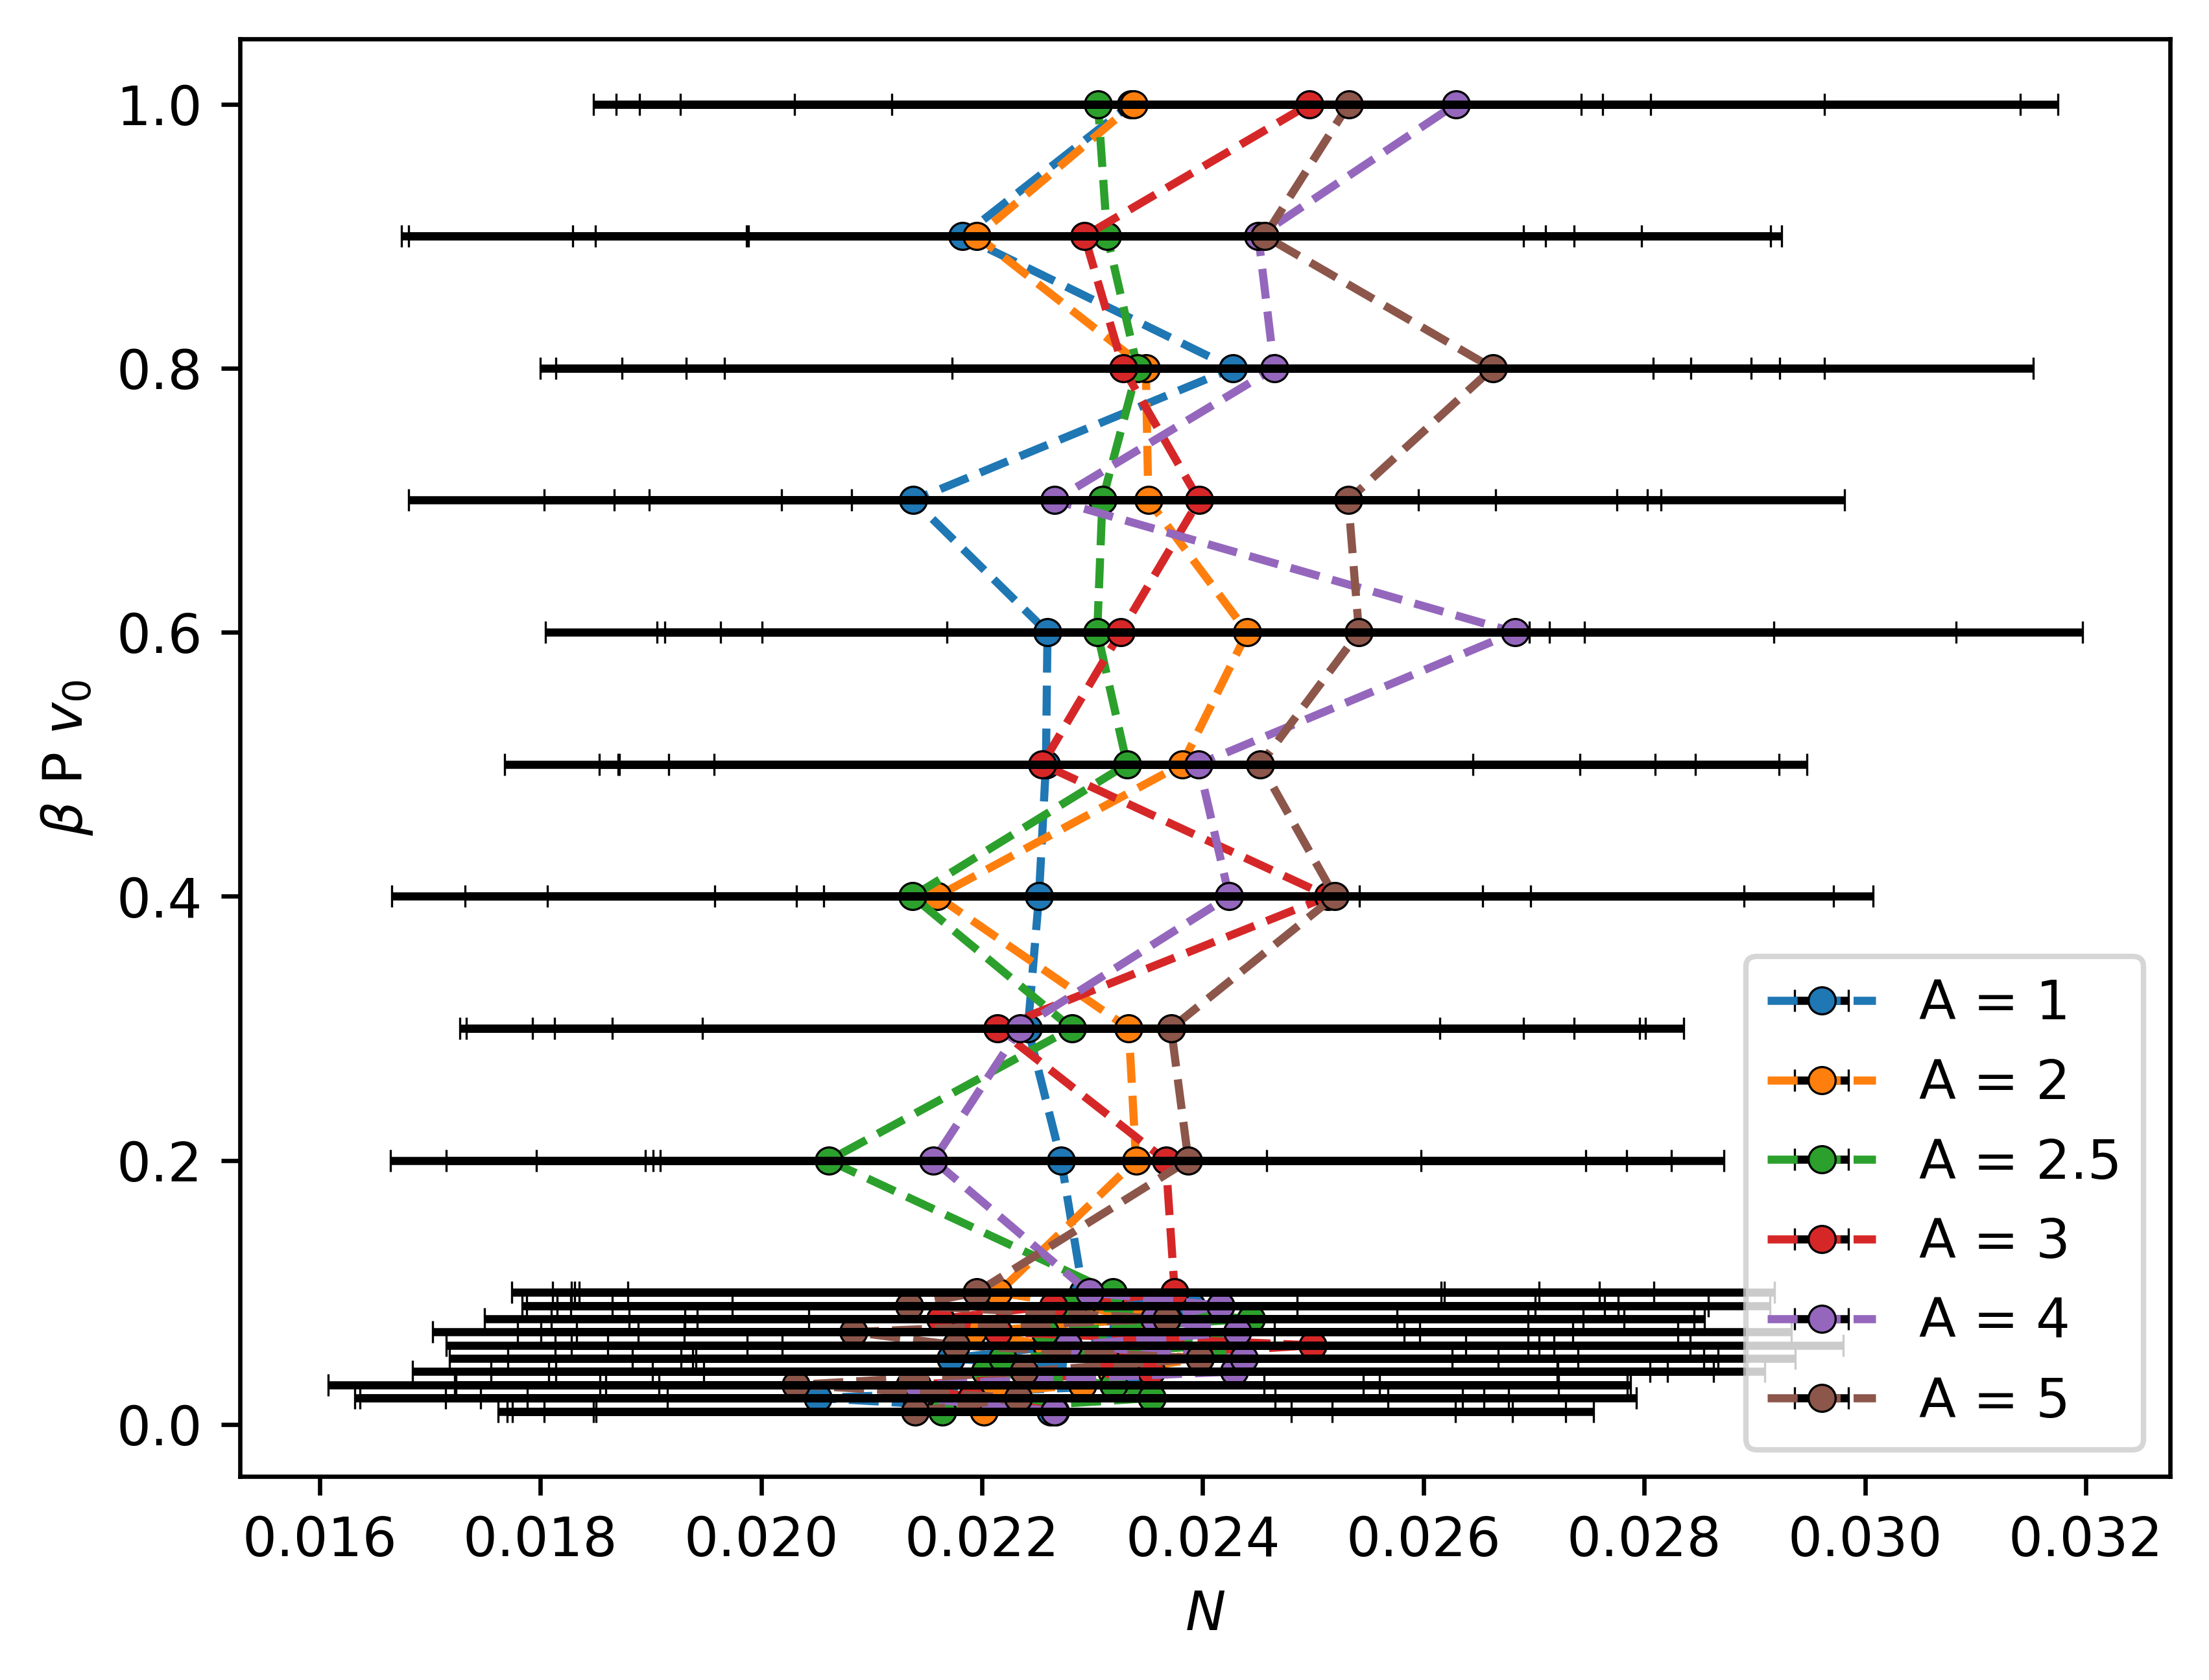
\includegraphics[width=0.3 \columnwidth]{Figures/S/PolyDLGauss0.75.png}
    \caption{Nematic order parameter for the different systems as a function of the particle elongation and reduced pressure of the system. (STESSE MODIFICHE DELL'IMMAGINE PRIMA)}
    \label{fig:S_par}
\end{figure}


%%%%%%%%

\section{Distribution functions $g(r)$ and $g_2(r)$}

The  radial pair distribution function $g(r)$ is defined as:
$$g(r) = \frac{1}{4 \pi \rho r^2 N} \sum_i \sum_{j \neq i} \delta(r - r_{ij})$$
where $\rho$ is the density of the system, N is the number of particles, $r_{ij}$ is the distance between the center of mass of the particles $i$ and $j$ and $\delta(r - r_{ij})$ is the Dirac function which gives $1$ if $r = r_{ij}$.

The orientational radial pair distribution function $g_2(r)$ unveils an eventual  angular correlation between couple of  particles as a function of the distance $r$ between their centres of masses: 
$$g_2(r) = \langle P_2 (\cos(\theta_{ij}(r))\rangle$$
where $P_2$ is the second order Legendre polynomial $P_2 (\cos(\theta_{ij}(r)) = (\cos^2(\theta_{ij}(r)) - 1)/2$, $\cos(\theta_{ij}(r)) = \boldsymbol{u}_i \cdot \boldsymbol{u}_j$,  and $\theta_{ij}(r)$ is the angle between the main axes  $\boldsymbol{u}_i$ and $\boldsymbol{u}_j$ of the $i$-th and $j$-th particles. 

At last, we explore the macroscopic orientational order of the system trough the nematic order parameter $S$, defined as the largest eigenvalue of the ordering matrix tensor $Q$:

$$Q = \frac{1}{2 N} \sum_i \left( 3 \langle (\textbf{u}_i)_\alpha (\textbf{u}_i)_\beta \rangle - \delta_{\alpha, \beta} \right)$$

where $\alpha \beta \in {x, y, z}$ and the unit vector $(\textbf{u}_i)_\alpha$ is the component $\alpha$ of the orientation of particle $i$.

While the nematic order parameter $S$ provides information over the emergence of an eventual ordering of the whole solution, $g(r)$ and $g_2(r)$ provide information over both the  arrangement and  alignment of the particles one with respect to the other. 

As expected, being all considered systems below the I-N transition, the nematic order parameter  is compatible with zero for all of the analysed systems, both monodisperse as well as polydisperse, thus no nematic order is to be expected in any of the solutions (as reported in detail in the SI).


The analysis of the pair distribution functions shows a strong dependence  of the properties of the solutions on $A$: the less the particle is elongated, the more the system behaves as a fluid of spheres [frenkel a caso]. As $A$ is increased, the first peak of the $g(r)$ gets reduced and shifted. This phenomenon might be a signature of a local pre-arrangement and the emergence of  the precursor of a preferred alignement between particles, due to their anisotropy, as shown in figure \ref{fig:G_Monodisperse}. 

\begin{figure}[!h]
    \centering
    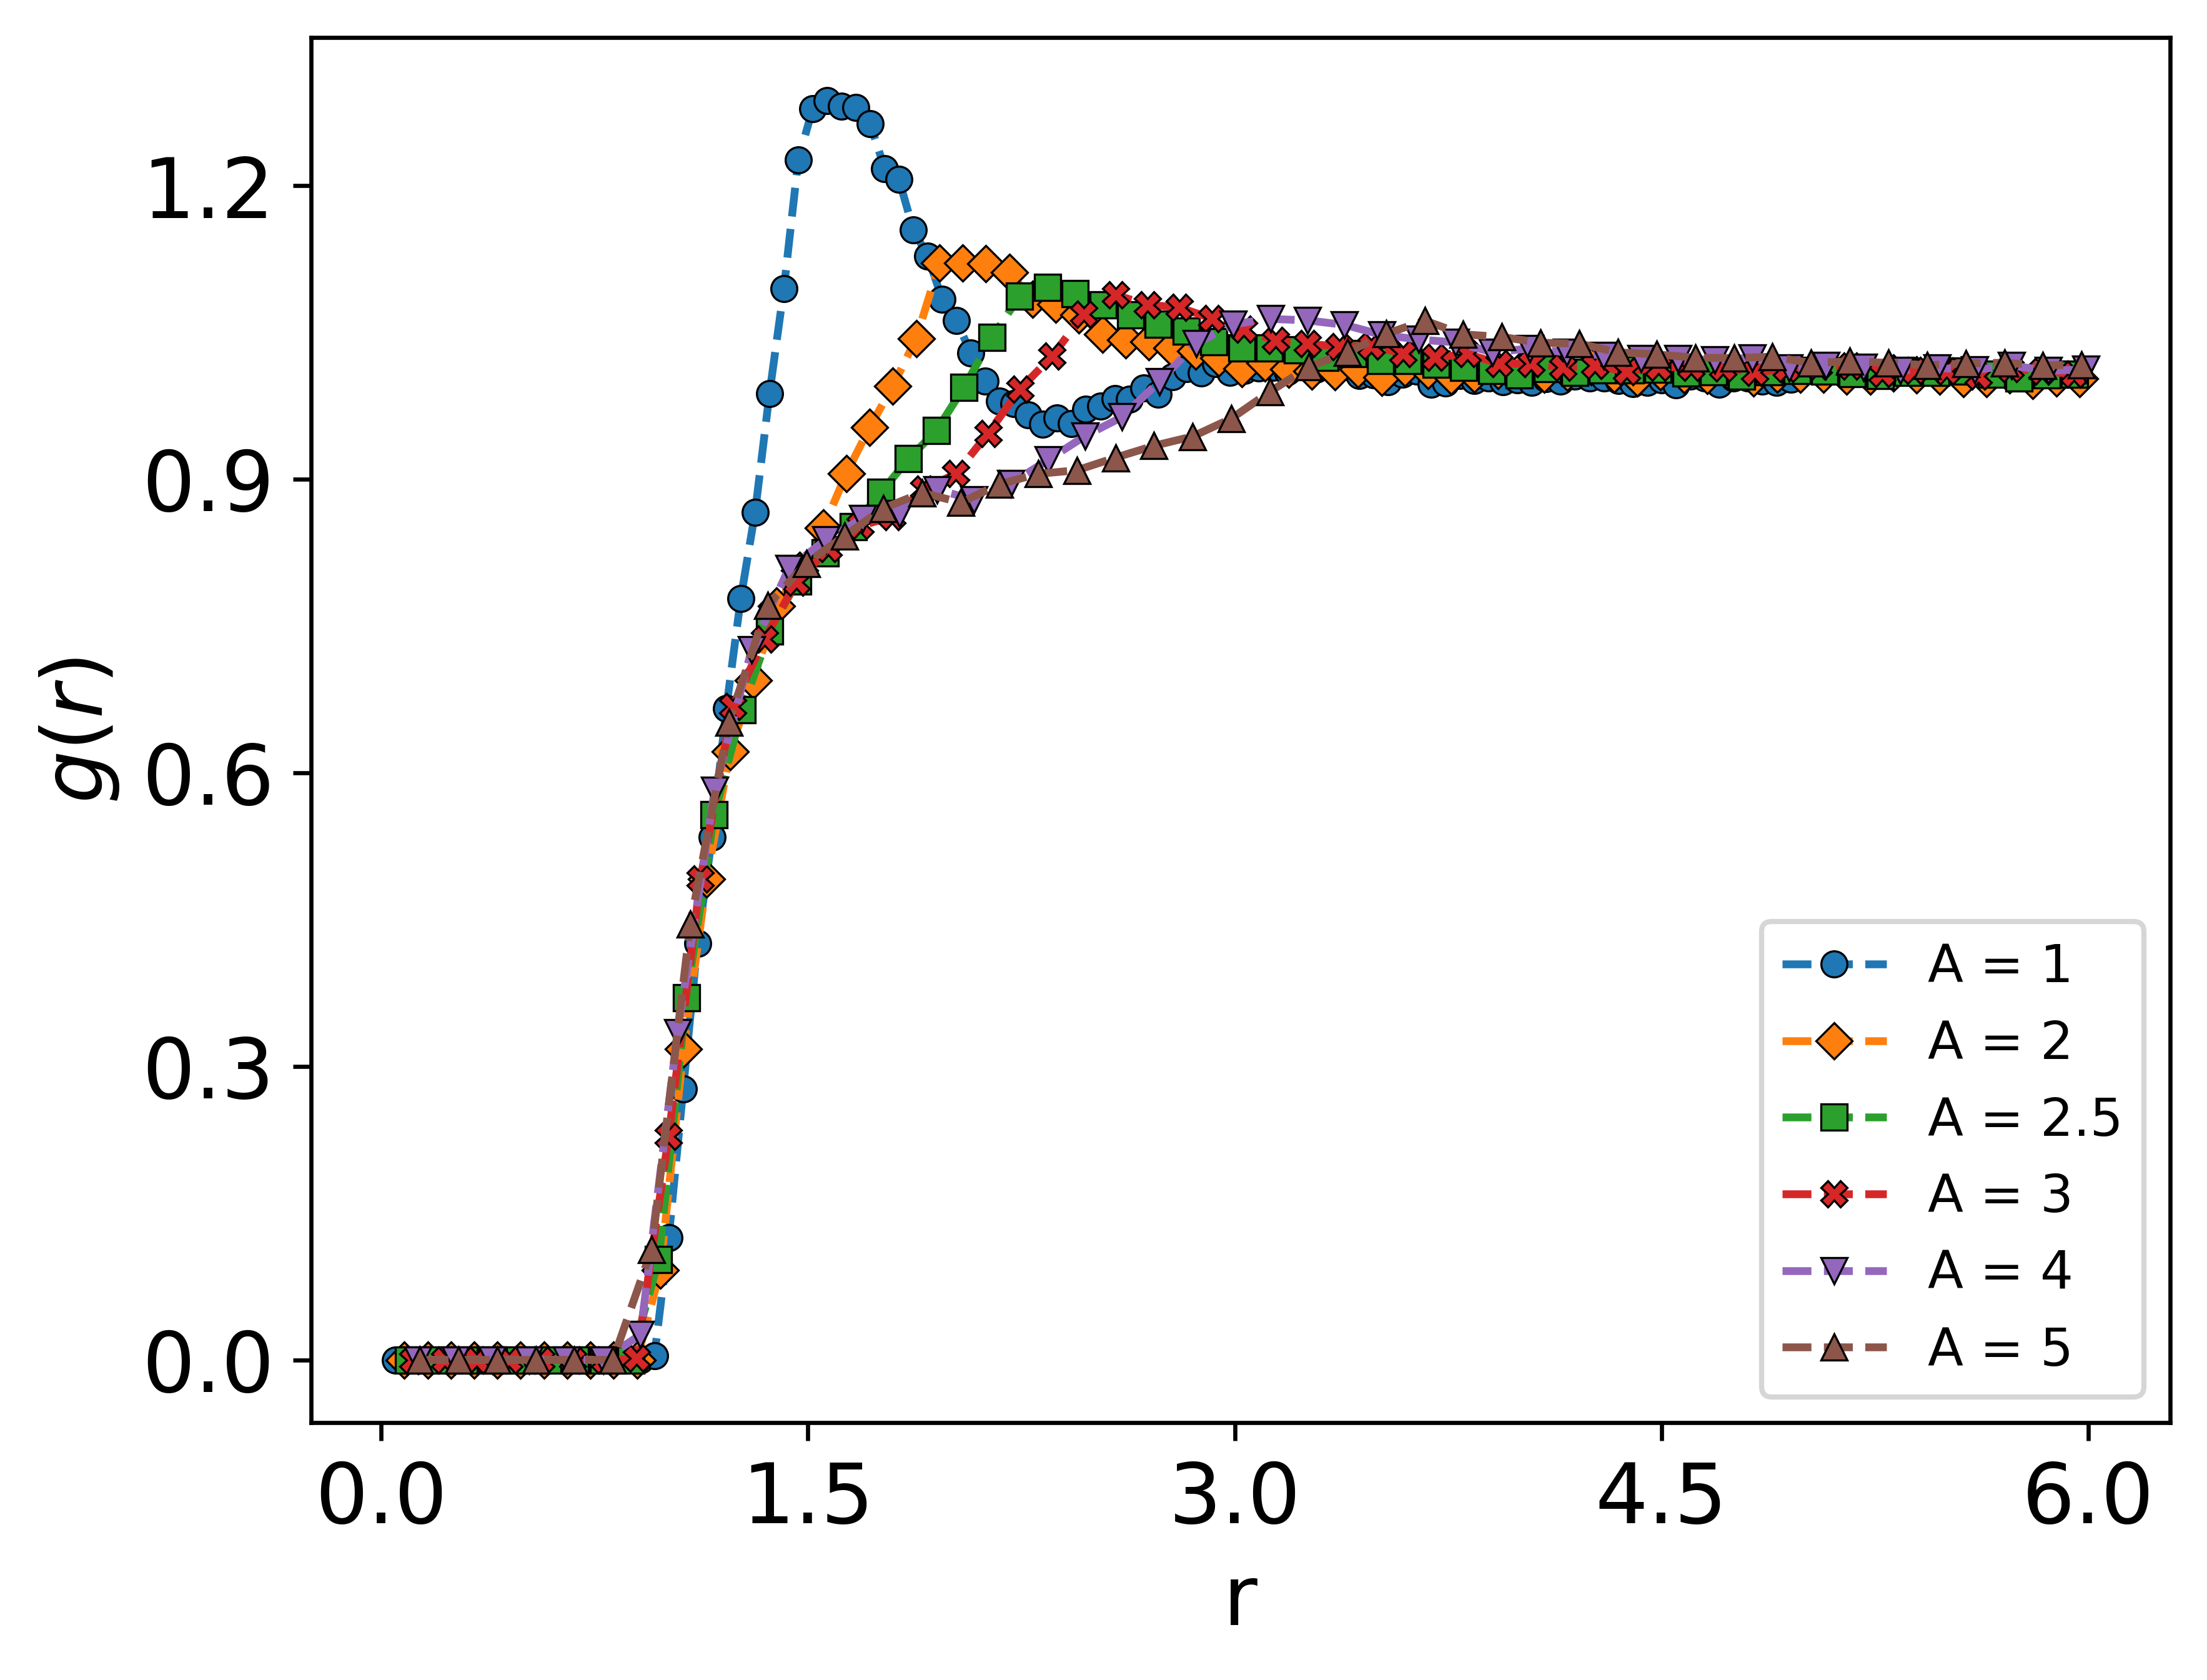
\includegraphics[width=0.45 \columnwidth]{Figures/G_mono.png}
    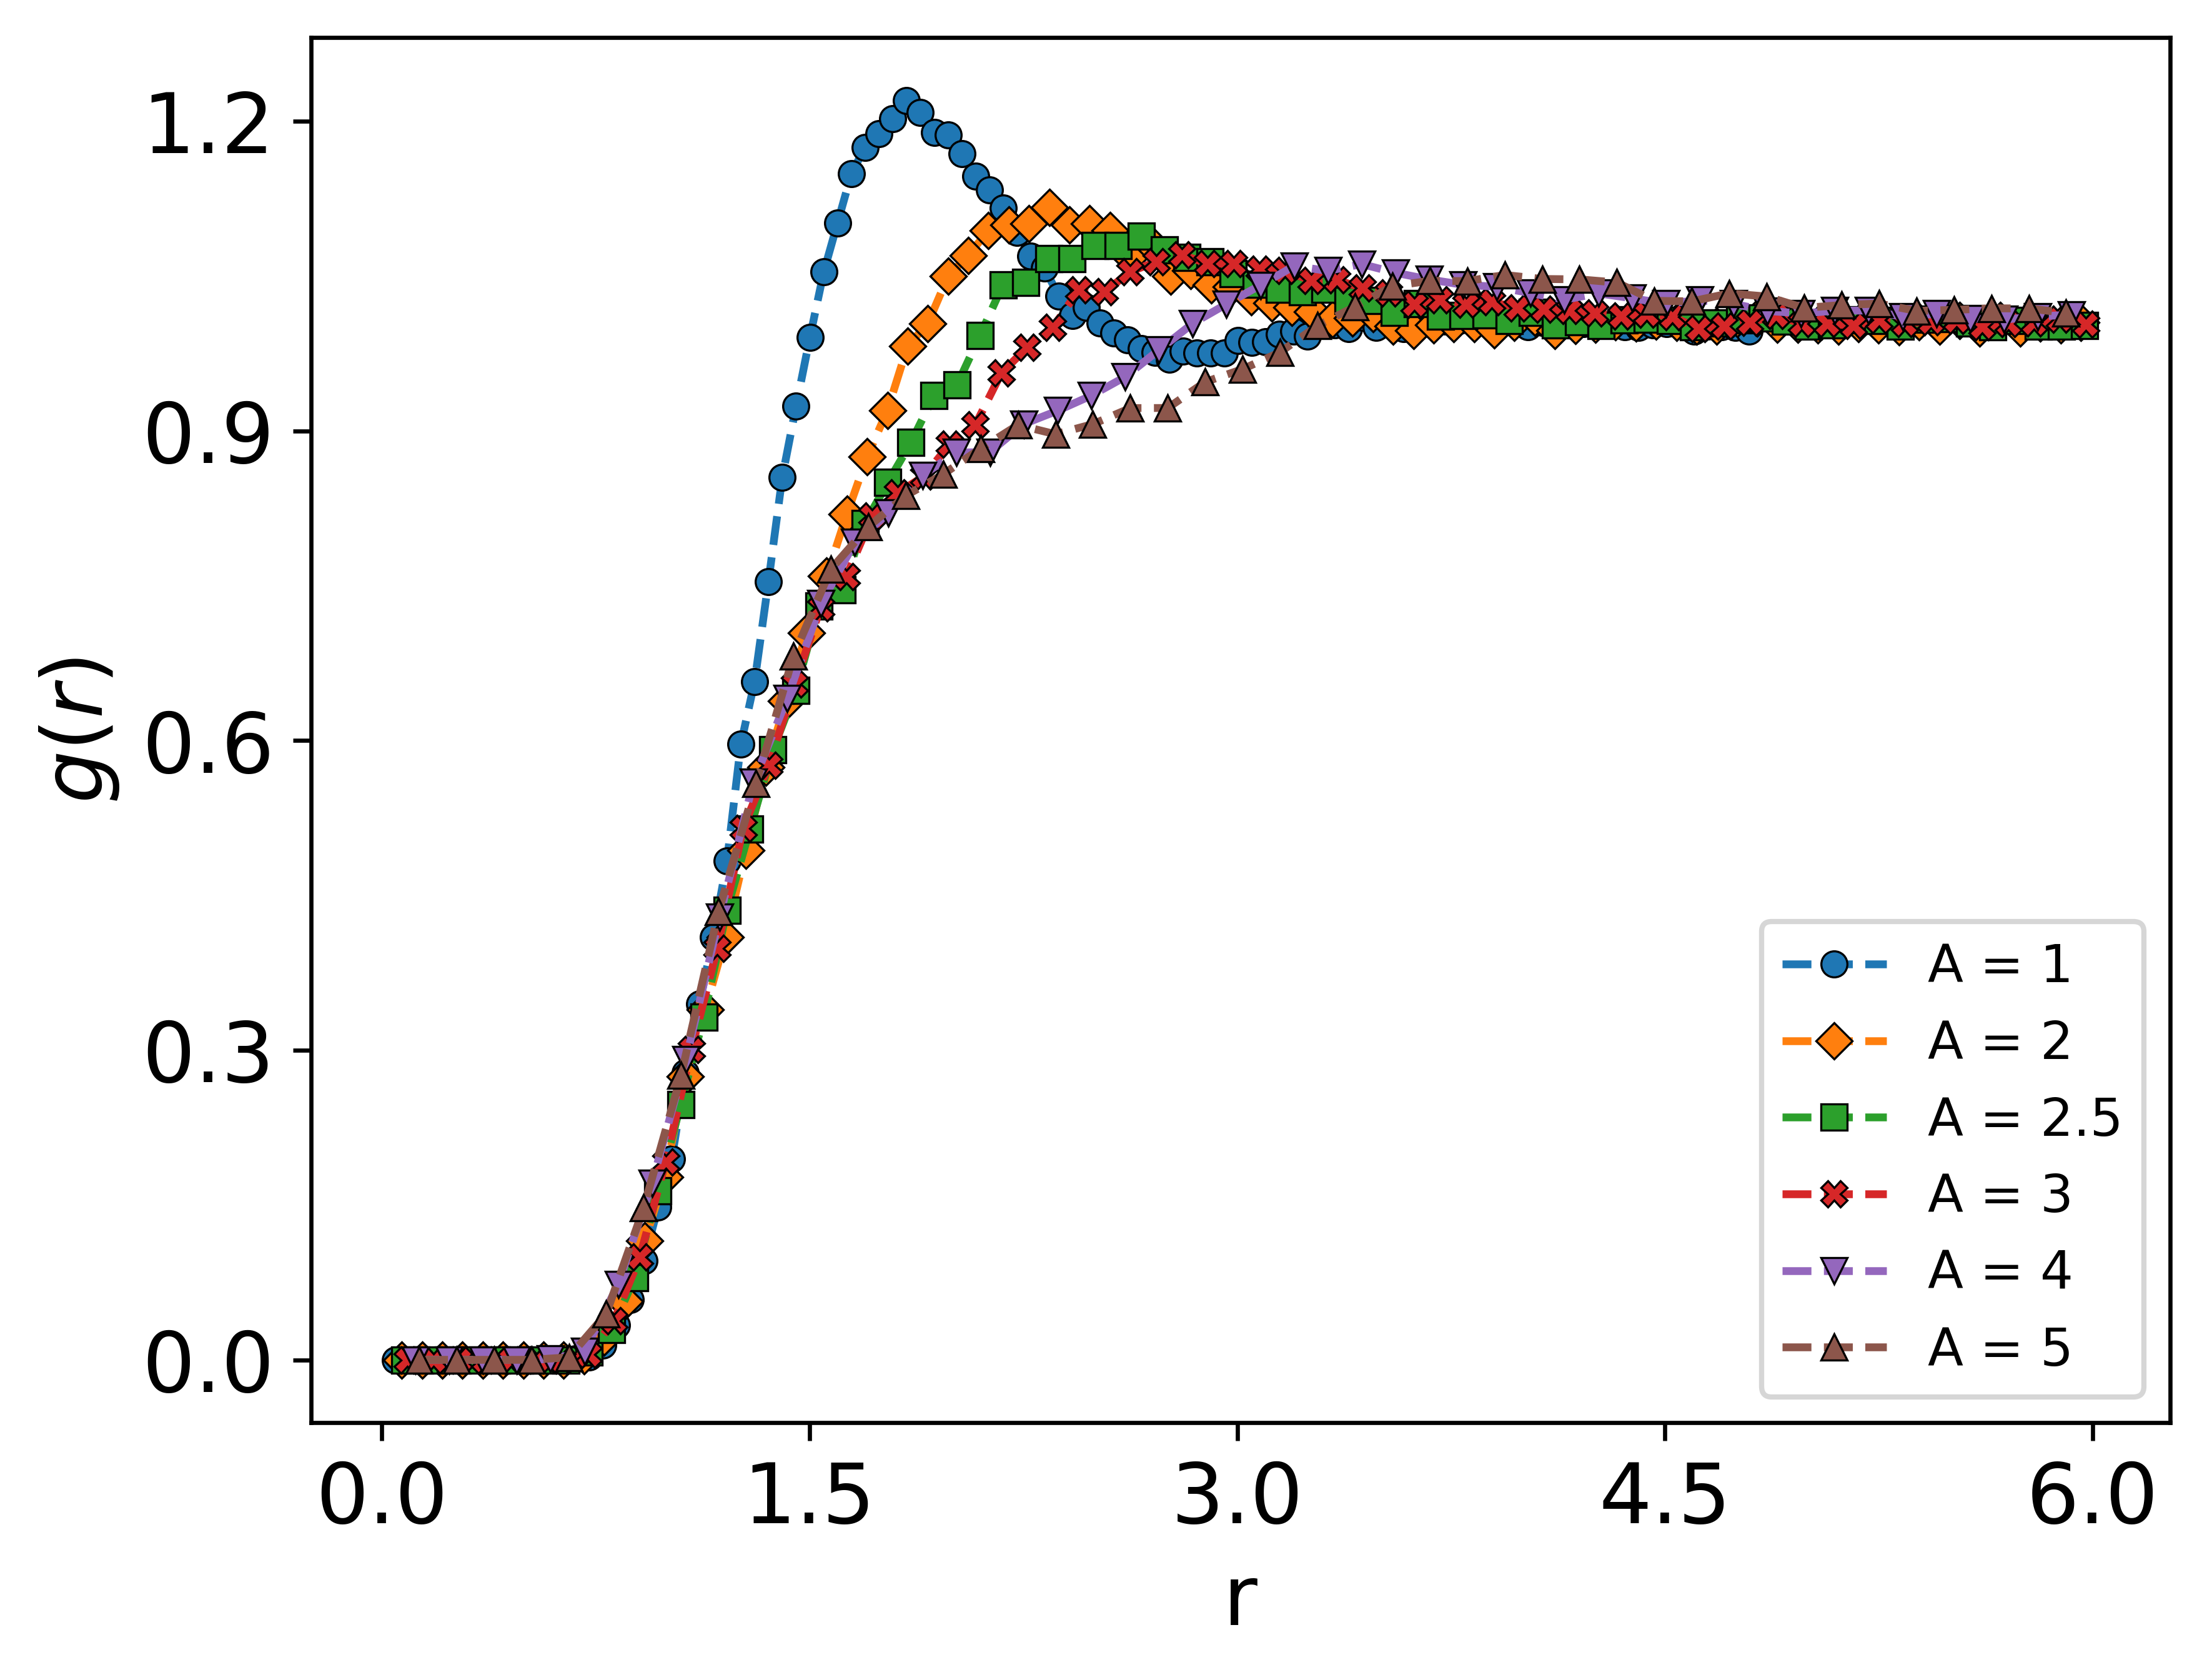
\includegraphics[width=0.45 \columnwidth]{Figures/G_polyD.png}
    \caption{Pair radial distribution function $g(r)$ as a function of the inter-particle distance $r$ for monodisperse systems (left) and with $PI_D = 50 \%$ (right) with different aspect ratio.}
    \label{fig:G_Monodisperse}
\end{figure}


Such phenomenon is not affected by the polydipersity for any $A$. We report in \ref{fig:G_comparison}  the comparison between all cases for $A=5$ and the rest in SI - riscrivere bene


\begin{figure}[!h]
    \centering
    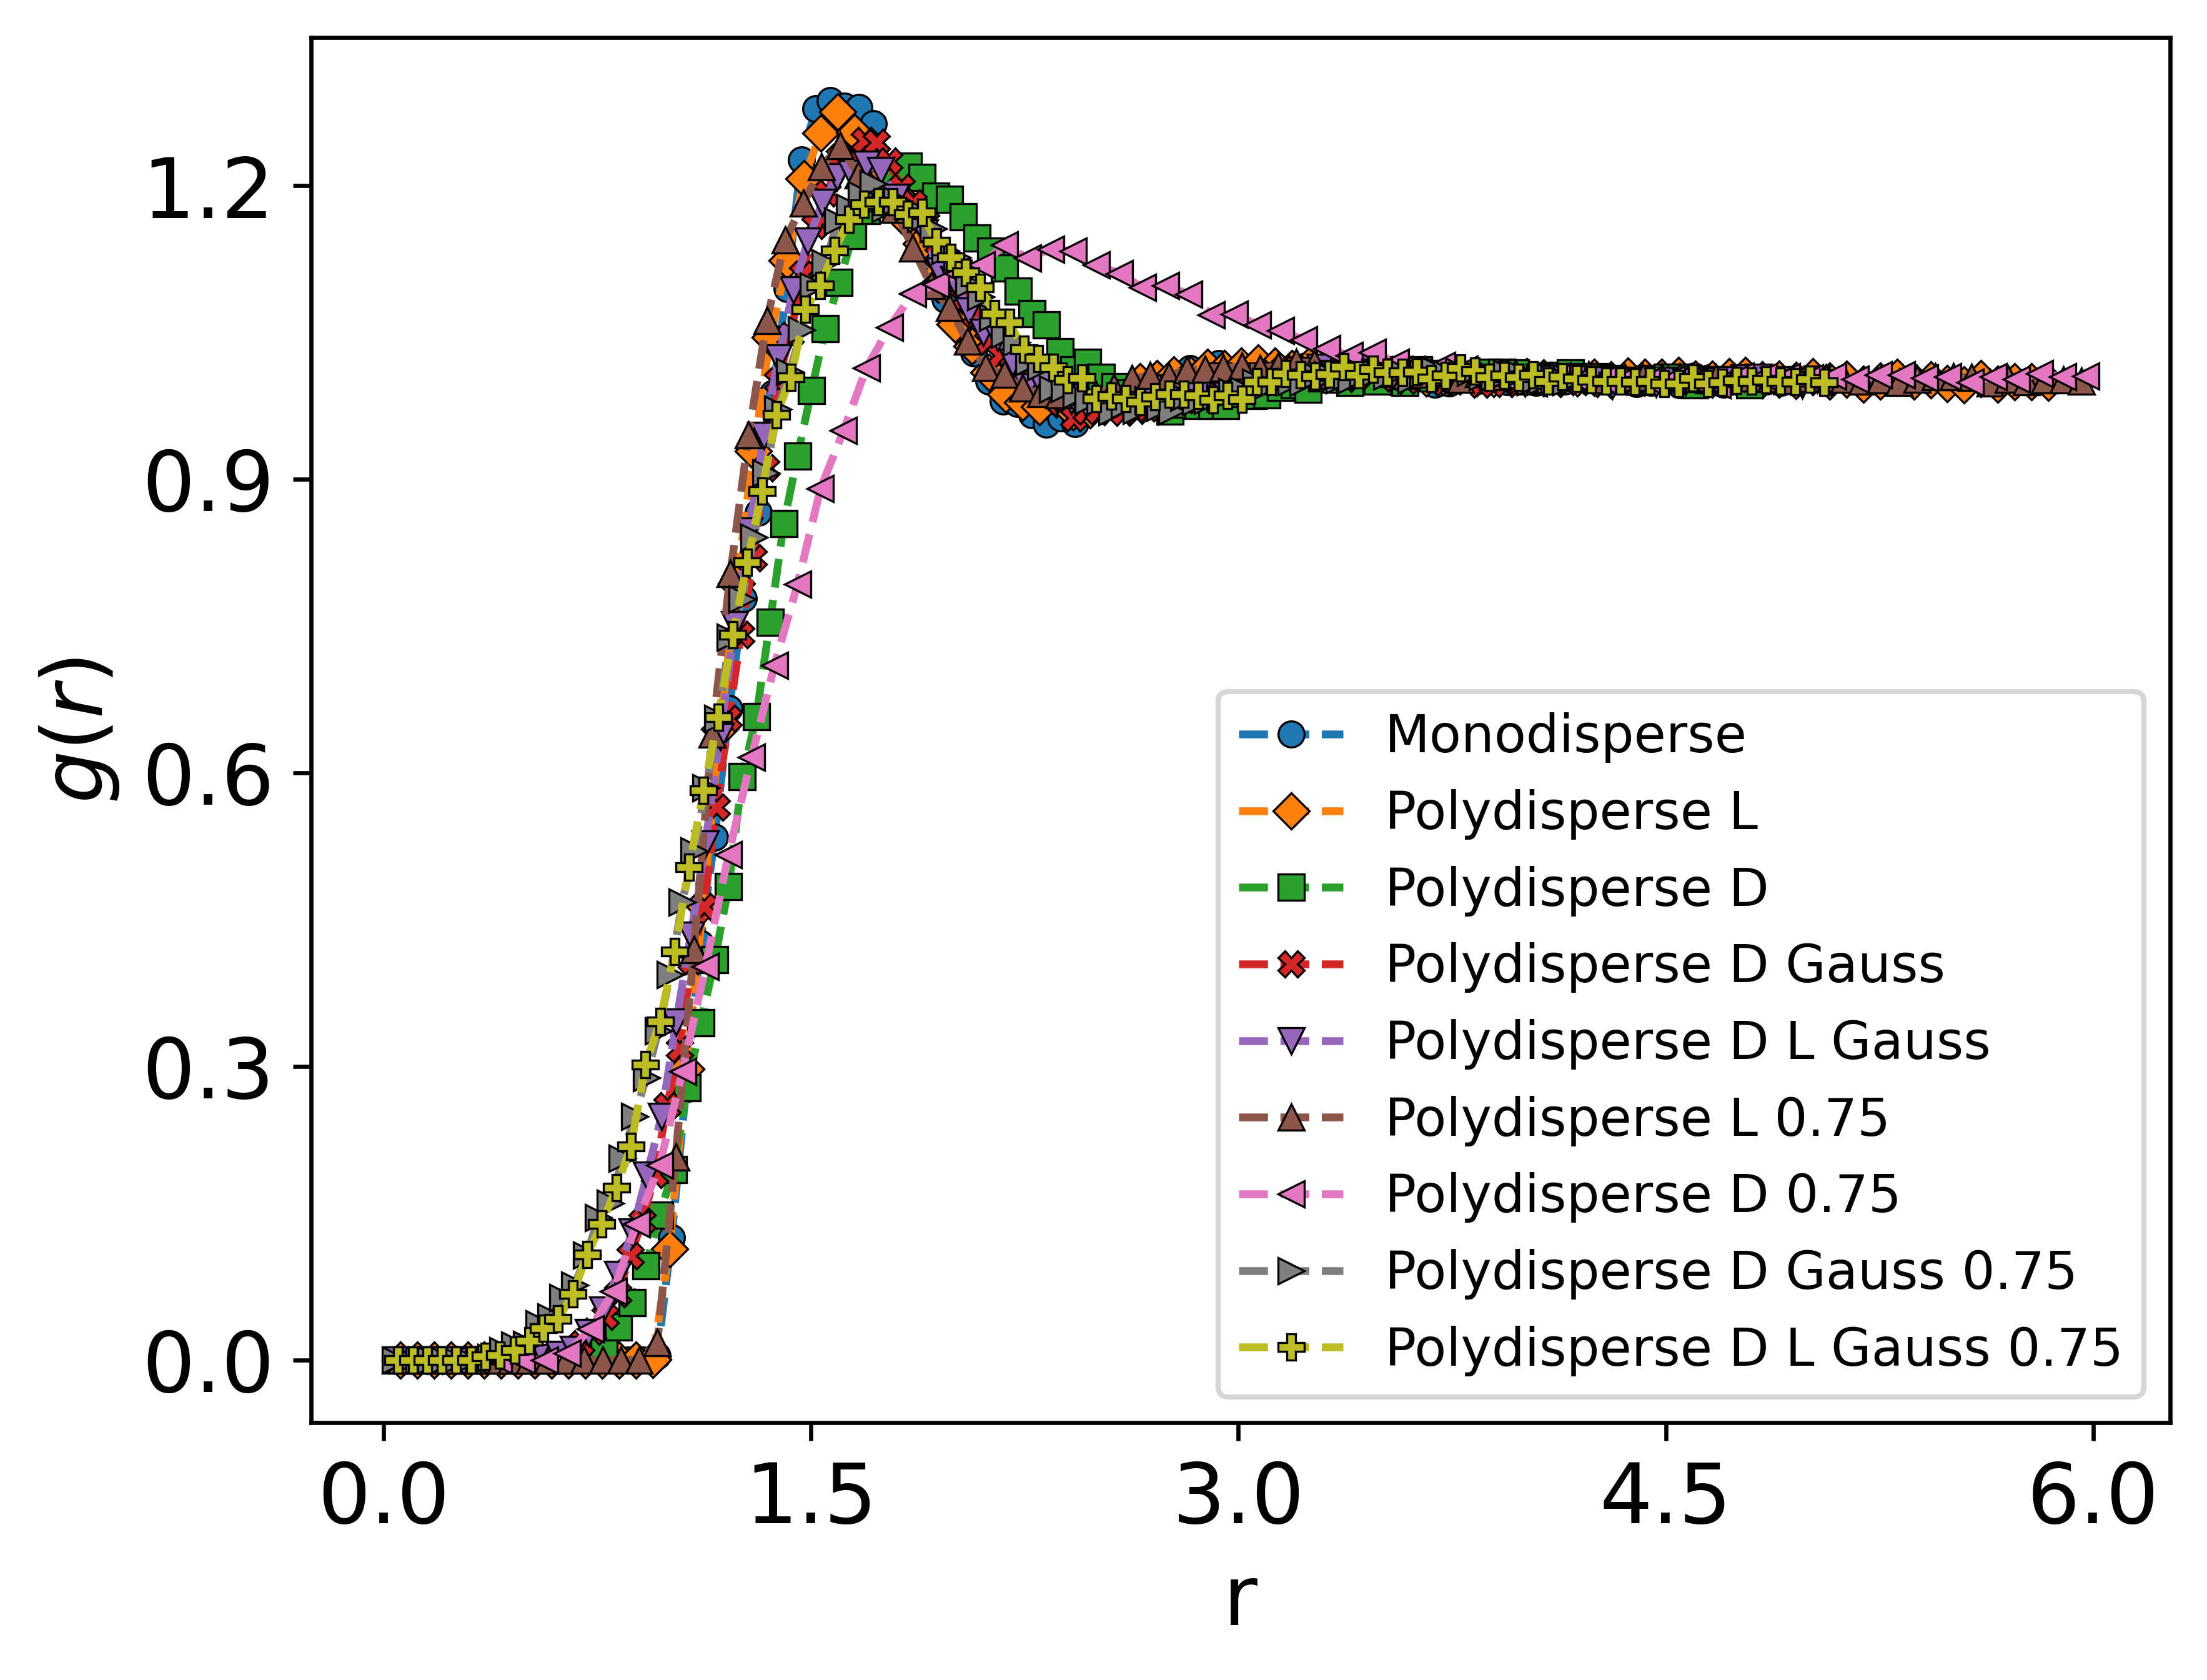
\includegraphics[width=0.45 \columnwidth]{Figures/G_A1.png}
    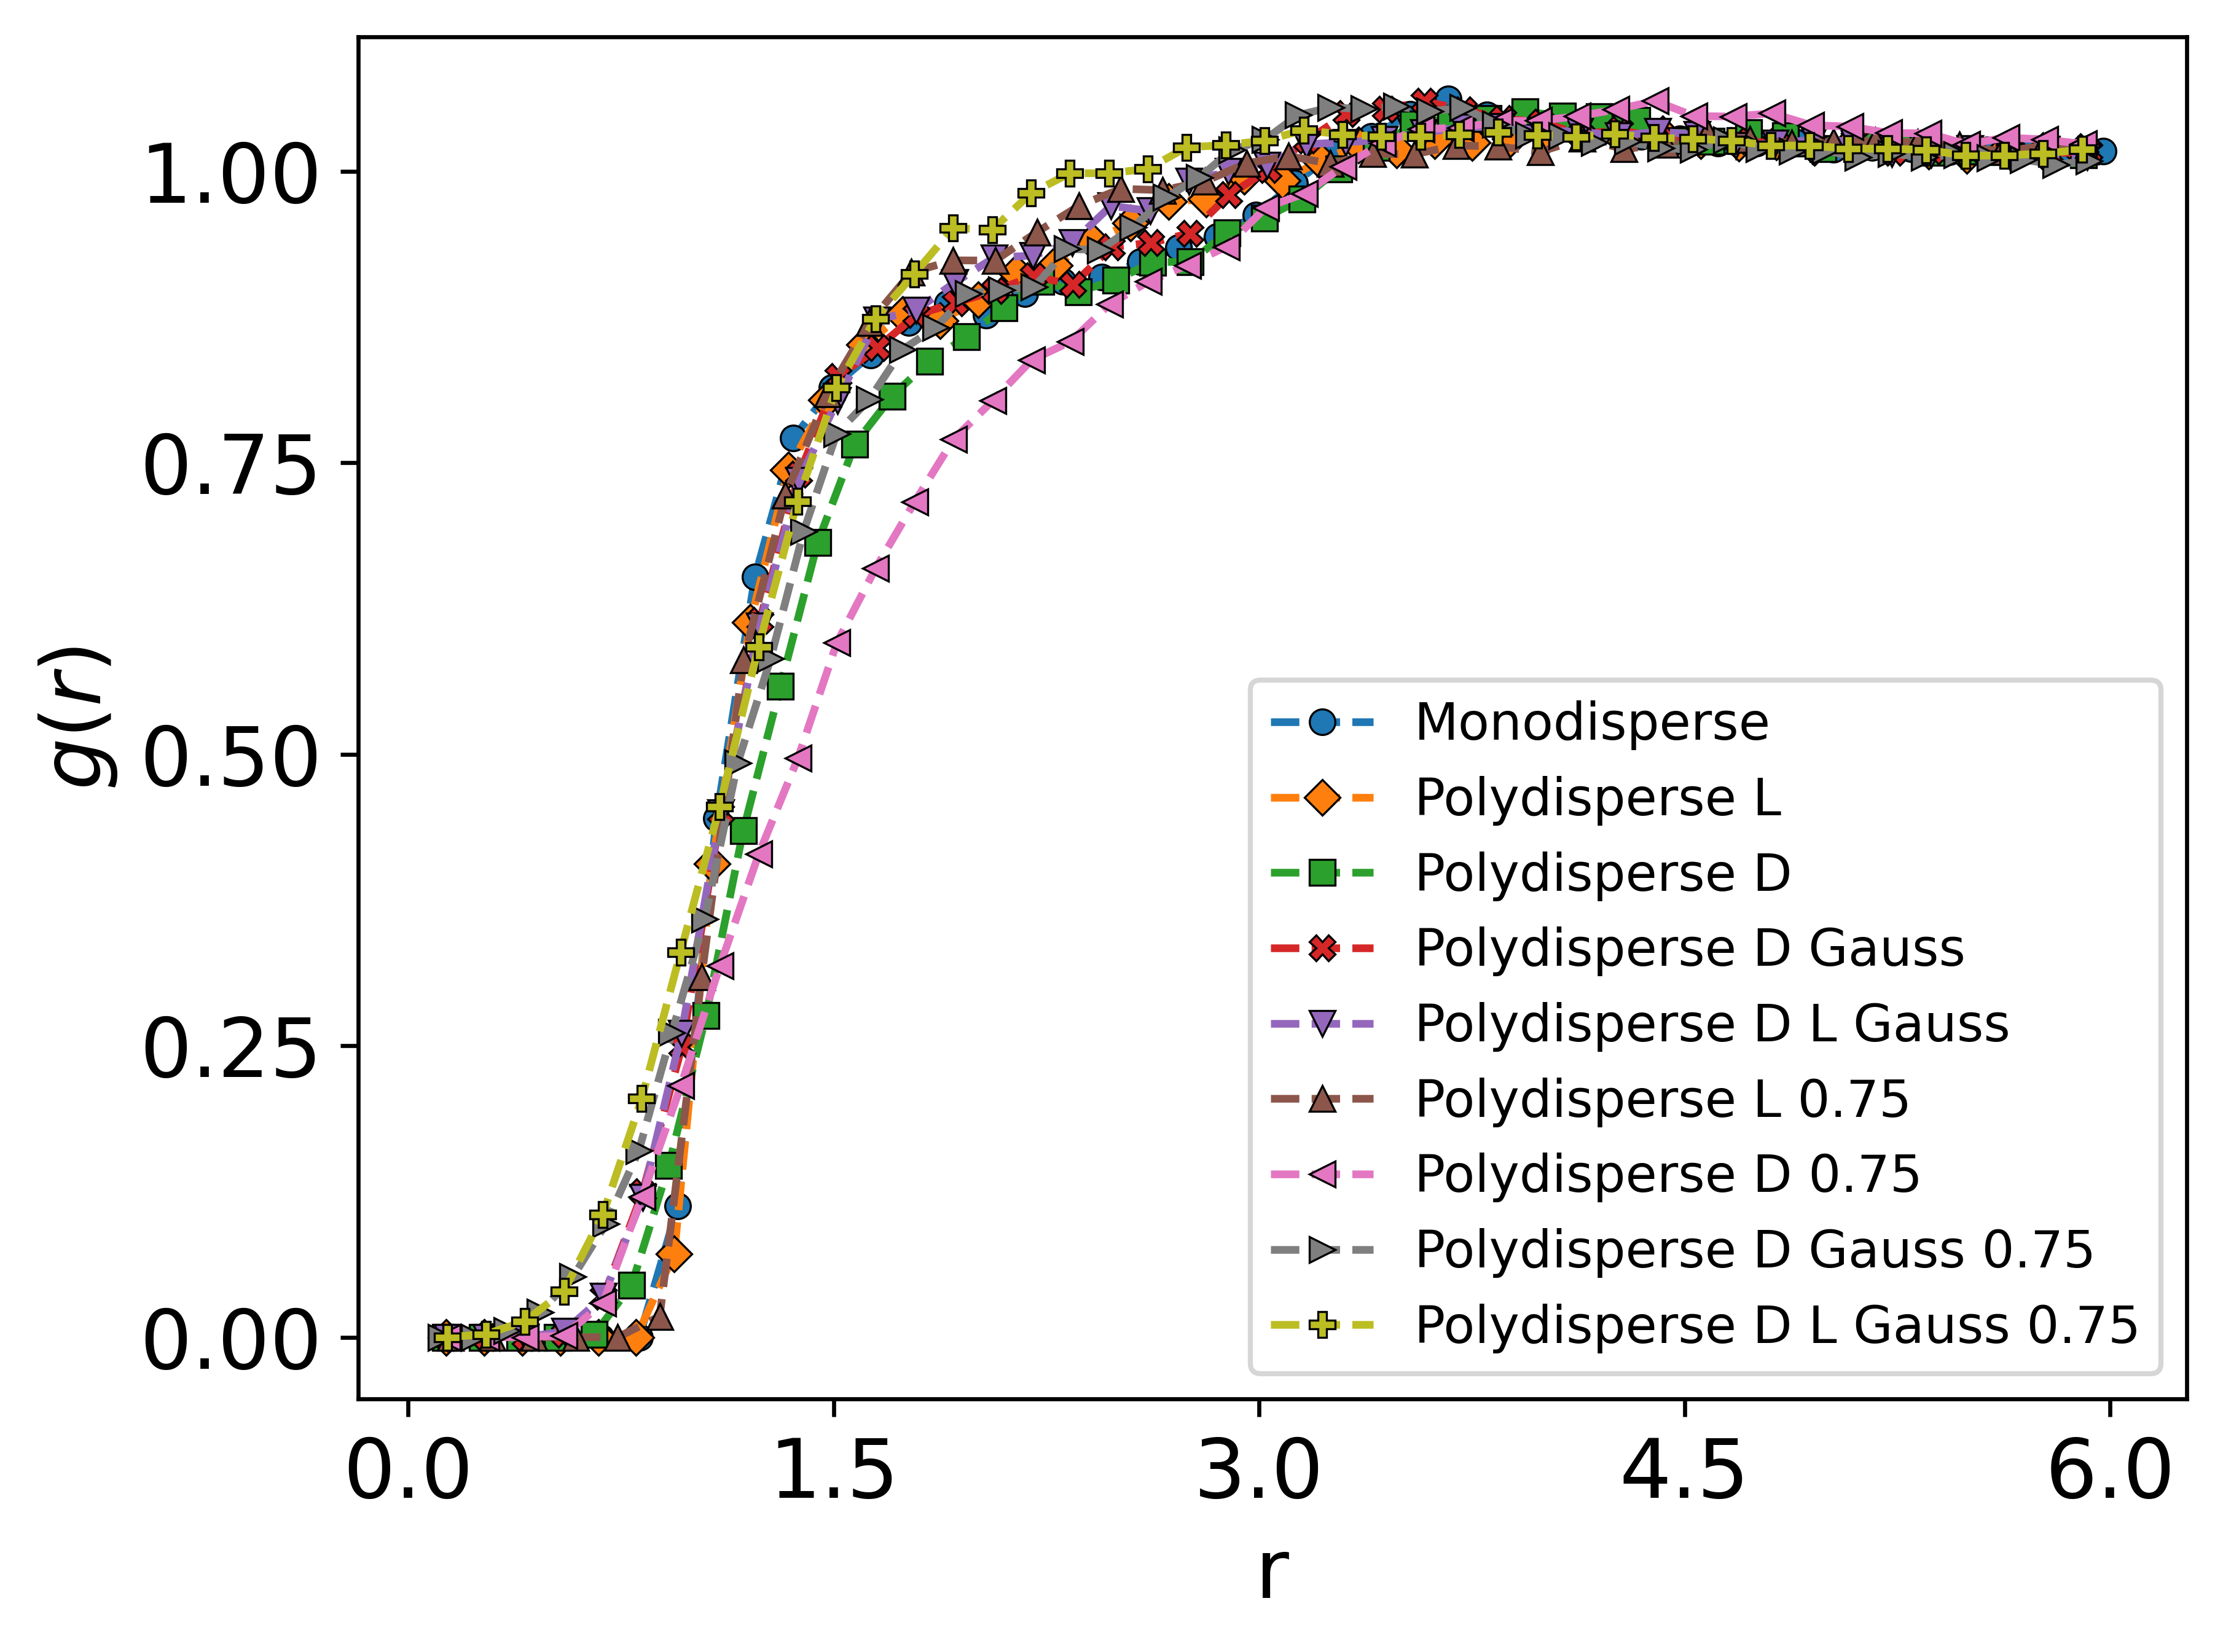
\includegraphics[width=0.45 \columnwidth]{Figures/G_A5.png}
    \caption{Pair radial distribution function $g(r)$ as a function of the inter-particle distance $r$ with $P^* = 1$ for the systems analysed in this work for $A = 1$ (left) and $A = 5$ (right).}
    \label{fig:G_comparison}
\end{figure}



To assess whether the effect of the polydispersity on the EOS is due to the emergence of local alignment, we focus on the orientational pair distribution function; if particles are completely aligned, $g_2(r)=1$, whether if particles are not aligned at all $g_2(r)=0$. 

%The exam of this parameter appears to be quite interesting in unveiling one of the reasons behind the different role played by a polyldispersity in $D$ and in $L$ on the EOS: as soon as pressure (or the packing fraction) is high enough (POSSIAMO QUANTIFICARE MEGLIO?) for particles to interact in average with one another, particles start aligning along their elongated axis. The bigger $A$, the stronger the alignment effect.
%FIGURE
The analysis of $g_2(r)$ shows that, notwithstanding no global nematic order is present in the system, anysotropy introduces the breaking of the global symmetry with a consequent local pre-ordering between particles, even in extremely dilute solutions. We saw such a phomenon in the dried TEM images reported in figure\ref{fig:tem}, where particles dried from extremely diluted solutions, show a local alignment along their principal axis. 

We can thus make a first comment on the fact that since particles are aligned parallel to $L$, but the low packing fraction considered do not present any long range order, a polydispersity in $L$ does not affect the global properties of the solution. 
Differently, the polydispersity in $D$ plays a  role, given that - due to the emergent pre-alignement - the average distance between particles is dominated by $D$. For such a reason not only the polydispersity in $D$ changes the global properties of the solution, but different polydispersities introduce different effects, as was pre-announced in the EOS shown in Figure \ref{fig:EOS_HSC_comparison}. Moreover no polydispersity influences the presence of local alignment between particles; the effect of a polydispersity in the diameter is shown in the width of the distribution, as shown for the $A=5$ case in figure\ref{fig:G_or_A5}

  \begin{figure}[!h]
    \centering
    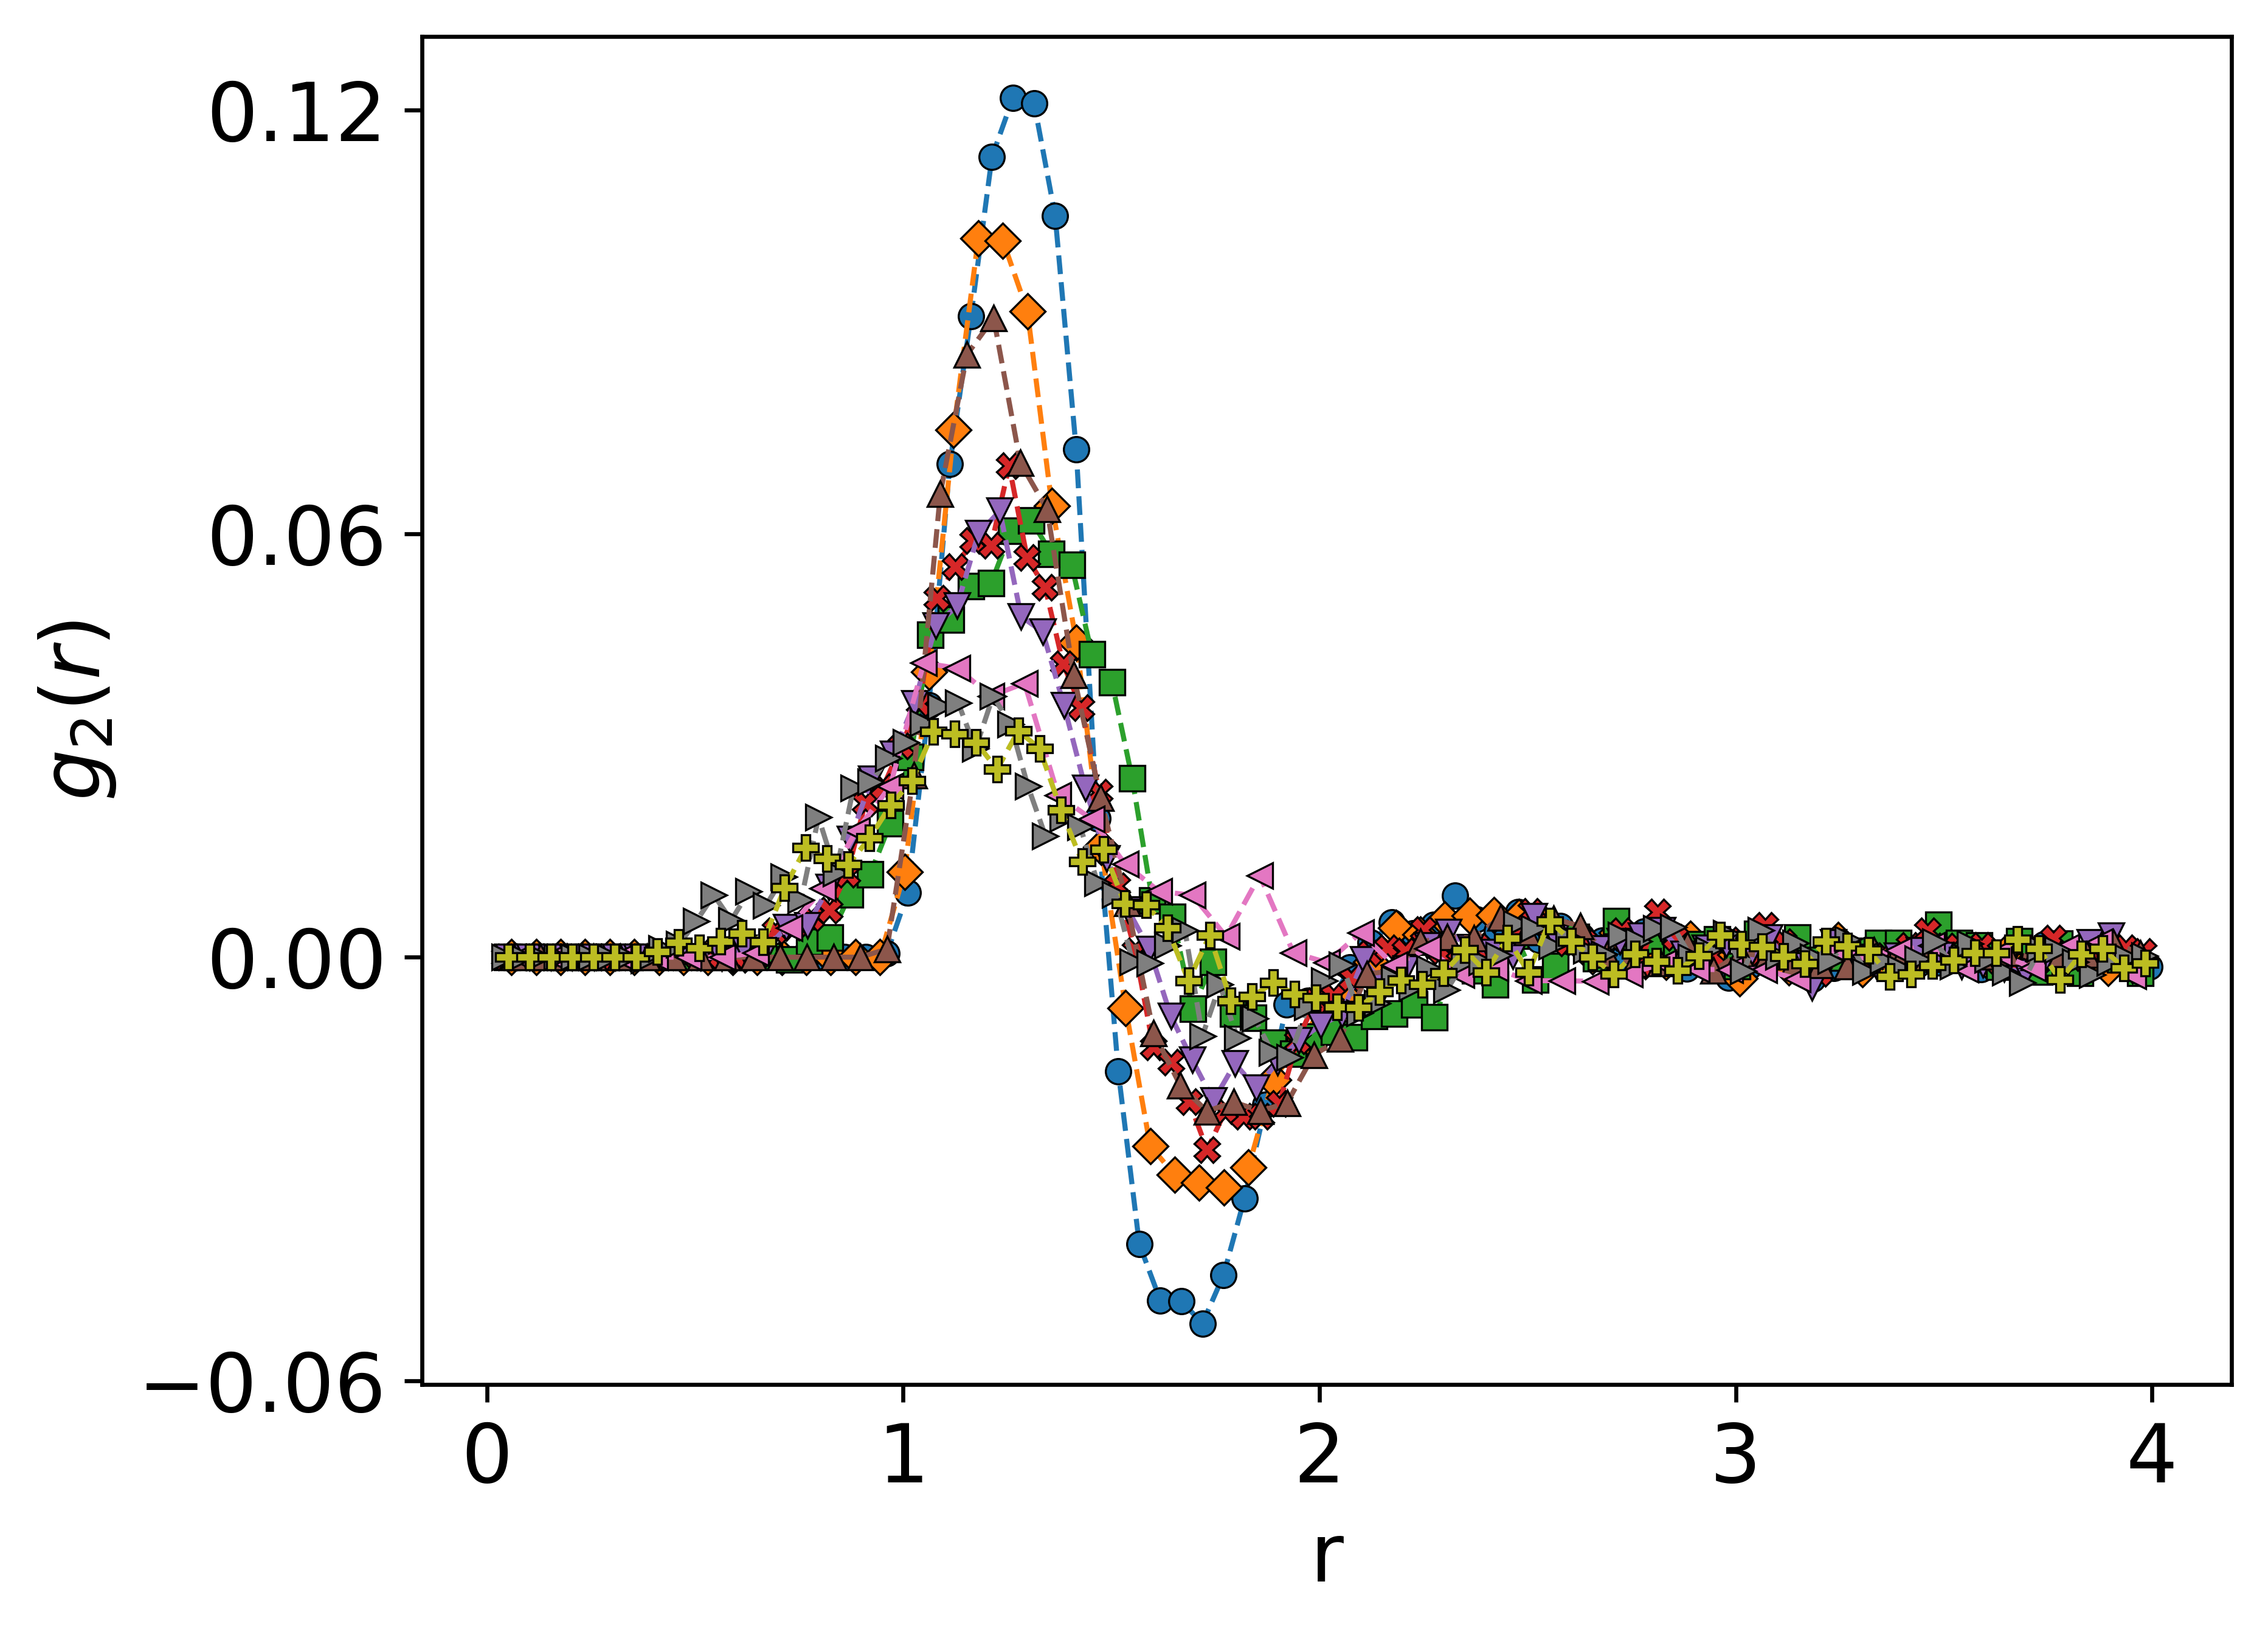
\includegraphics[width=0.45 \columnwidth]{Figures/G_or_A1.png}
    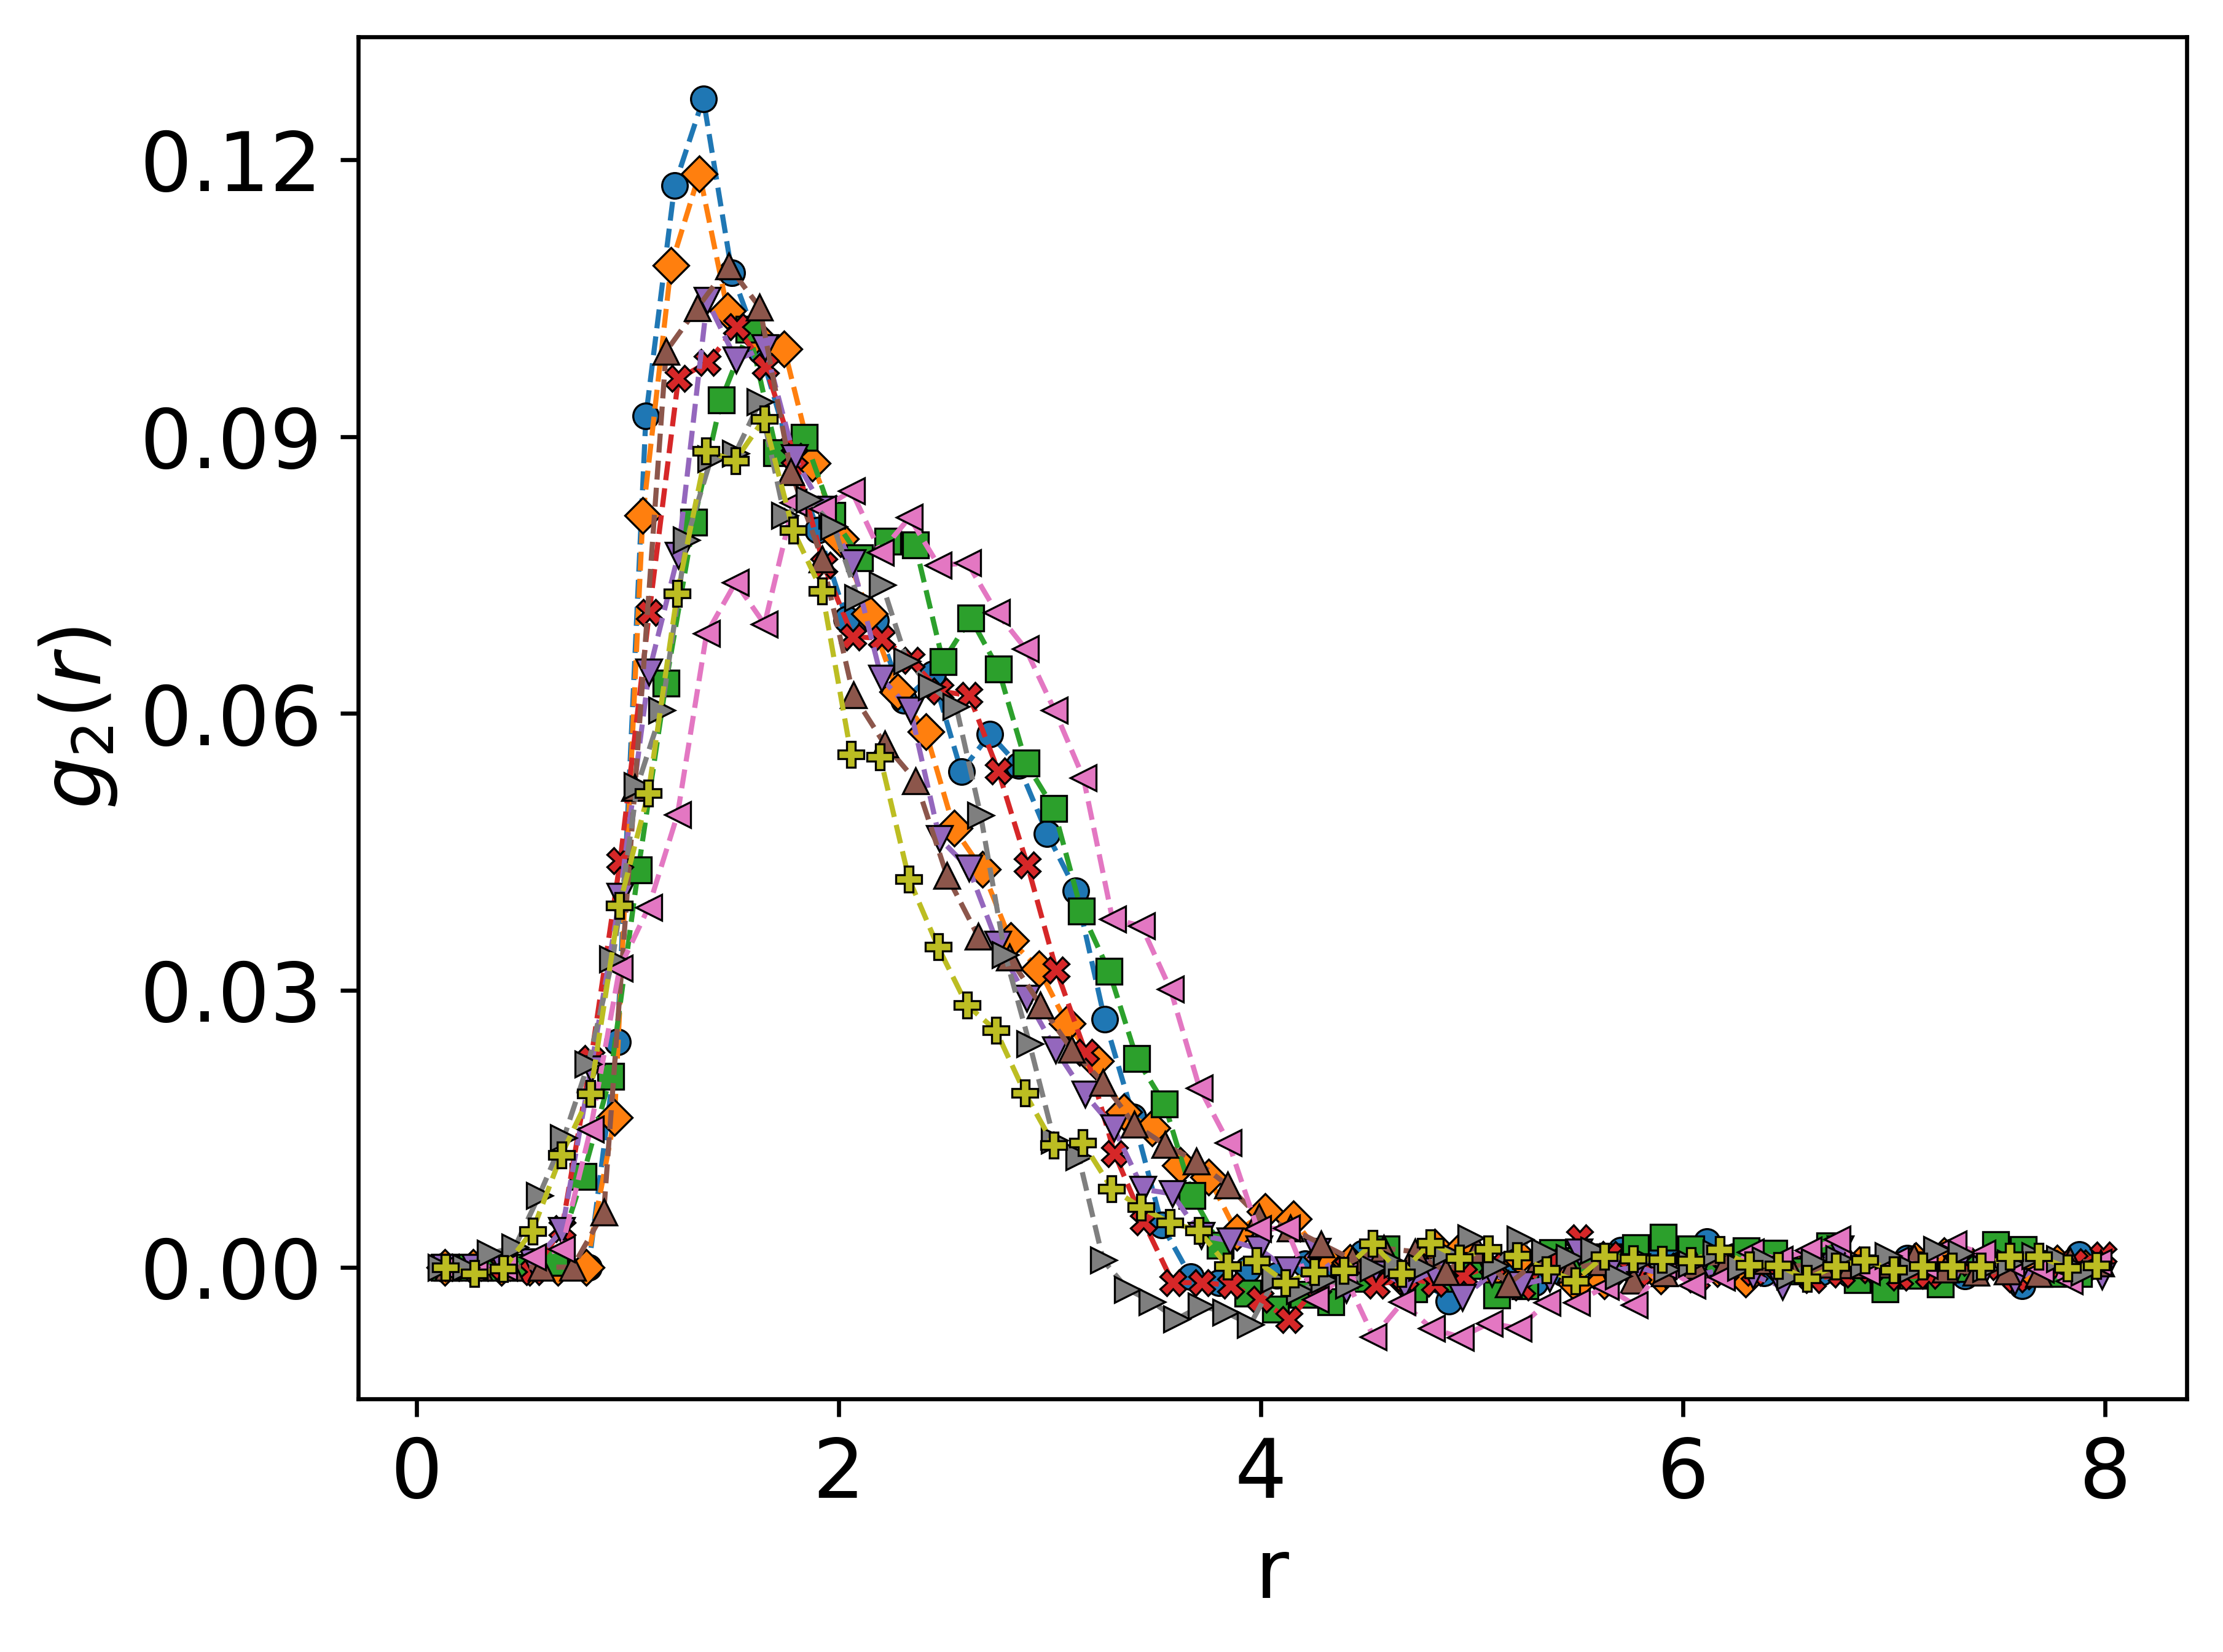
\includegraphics[width=0.45 \columnwidth]{Figures/G_or_A5.png}
    \caption{Orientational pair radial distribution function $g_2(r)$ as a function of the inter-particle distance $r$ for the systems considered in this paper.}
    \label{fig:G_or_A5}
\end{figure}
 
 

We now move to a more theoretical investigation of the system exploiting the theoretical approach introduced in the previous section.



\begin{comment}
\section{Radial pair distribution function $g(r)$}

\begin{figure}[!h]
    \centering
    \includegraphics[width=0.5 \columnwidth]{Figures/G_or_Monodisperse.png}
    \caption{}
    \label{fig:G_or_Monodisperse}
\end{figure}

\section{Orientational radial pair distribution function $g_2(r)$}

Another interesting information grasped by the $g_2(r)$ is the effect on the local arrangement due to a change in  $A$ (see Figure \ref{fig:G_or_Monodisperse}) - commentala un poco 

\begin{figure}[!h]
    \centering
    \includegraphics[width=0.5 \columnwidth]{Figures/G_or_Monodisperse.png}
    \caption{Orientational pair radial distribution function $g_2(r)$ as a function of the inter-particle distance $r$ for monodisperse systems with different aspect ratio.}
    \label{fig:G_or_Monodisperse}
\end{figure}

\begin{figure}[!h]
    \centering
    \includegraphics[width=0.6 \columnwidth]{Figures/PL_mono_5.png}
    \caption{EOS of monodisperse system of spherocylinders of A = 5. The lines correspond to: ideal gas ($P^* = \phi$), virial expansion ($P^* = \phi + \phi^2 \frac{\overline{v_{excl}}}{2 v_0}$) and Parson-Lee approximation as in Eq.\ref{ParsonLee}. }
    \label{fig:Theory_comp_A5}
\end{figure}


\begin{figure}[!h]
    \centering
    \includegraphics[width=0.6 \columnwidth]{Figures/Monodisperse_PL.png}
    \includegraphics[width=0.6 \columnwidth]{Figures/PolydisperseD_PL.png}
    \caption{EOS of a monodisperse system (left) and with a polydispersity in D (right) for different aspect ratios. The lines correspond to the Parson-Lee approximation as in Eq.\ref{ParsonLee}. }
    \label{fig:PL_5_mono}
\end{figure}

\end{comment}

\section{Average particle volume and excluded volume}

In this section is shown the calculation of the average excluded volume $\overline{v_{excl}}$ of a system of polydisperse hard spherocylinders in the isotropic phase and its average particle volume $\overline{v_0}$.

The excluded volume of two spherocylinders of length $(L_1, L_2)$ and diameter $(D_1, D_2)$ is a function of the angle $\gamma$ between their main axes [Onsager 1949]:

\begin{equation} \label{eq:vexcl}
    v_{excl}(\gamma[\Omega_1, \Omega_2]) = \frac{4}{3} \pi \left(\frac{D_1 + D_2}{2}\right)^3 + \pi \left(\frac{D_1 + D_2}{2}\right)^2 (L_1 + L_2) + 2 \left( \frac{D_1 + D_2}{2} \right) L_1 L_2 \sin(\gamma)
\end{equation}

As already wrote in the main text (credo che non vada bene detta così), we can calculate the average excluded volume as:

\begin{equation}
	\overline{v_{excl}}  = \iint v_{excl}(\gamma[\Omega_1, \Omega_2]) f(\Omega_1)f(\Omega_2) d\Omega_1 d\Omega_2    
\end{equation}

The orientational distribution function for the isotropic phase is equal to $f(\Omega) = 1 / (4 \pi)$, thus the integral over the solid angles $\Omega_1$ and $\Omega_2$ of the last term of Eq. \ref{eq:vexcl} gives

\begin{equation}
    \iint \sin{\left(\gamma[\Omega_1, \Omega_2]\right) f(\Omega_1) f(\Omega_2) d\Omega_1 d\Omega_2 =4 \pi^3} \frac{1}{16 \pi^2} = \frac{\pi}{4}
\end{equation}

and the average mutual excluded volume of two spherocylinders becomes:

\begin{equation} \label{eq:mean_vexcl}
    \overline{v_{excl}}(L_1, D_1, L_2, D_2) = \frac{4}{3} \pi \left(\frac{D_1 + D_2}{2}\right)^3 + \pi \left(\frac{D_1 + D_2}{2}\right)^2 (L_1 + L_2) + \frac{\pi}{2} \left( \frac{D_1 + D_2}{2} \right) L_1 L_2
\end{equation} 

In a monodisperse system the average excluded volume is given by

\begin{equation} \label{eq:vexcl_mono}
   \overline{v_{excl}}(L, D) = \frac{4}{3} \pi D^3 + 2 \pi D^2 L + \frac{\pi}{2} D L^2
\end{equation}

For a polydisperse system it is possible to obtain the mean excluded volume following two paths. The first, suitable for the analysis of simulation data, consists of averaging Eq. \ref{eq:mean_vexcl} on all possible the combinations of particles in the finite system:

\begin{equation}\label{Vexcl_poly}
    \overline{v_{excl}} = \frac{2}{N (N-1)} \sum_{i=1} ^N \sum_{j>i}^N \overline{v_{excl}}(L_i, D_i, L_j, D_j).
\end{equation}

The second involves the calculation of the integral by means of the probability distributions of the diameter $\rho(D)$ and length $\rho(L)$ of the sample:

\begin{equation}
    \overline{v_{excl}} = \iiiint \rho(L_1) \rho(L_2) \rho(D_1) \rho(D_2) \overline{v_{excl}}(L_1, L_2, D_1, D_2) dL_1 dL_2 dD_1 dD_2
\end{equation}

Analogously to the excluded volume, the average particle volume $v_0$ can be computed for a finite system as

\begin{equation}
    \overline{v_0} = \frac{1}{N} \sum_{i=1} ^N  v_0(L_i, D_i)
\end{equation}

or by using the probability distributions

\begin{equation}
    \overline{v_0} = \iint \rho(L) \, \rho(D) \, v_0(L, D) \, dL dD
\end{equation}

where $v_0(L, D) = \frac{\pi D^3}{6} + \frac{\pi D^2 L}{4}$ is the volume of a single particle of the system.


\section{Theory comparison}

Qualitative agreement between simulations and Parson-Lee theory for all the elongations analysed.

\begin{figure}[!h]
	\centering
	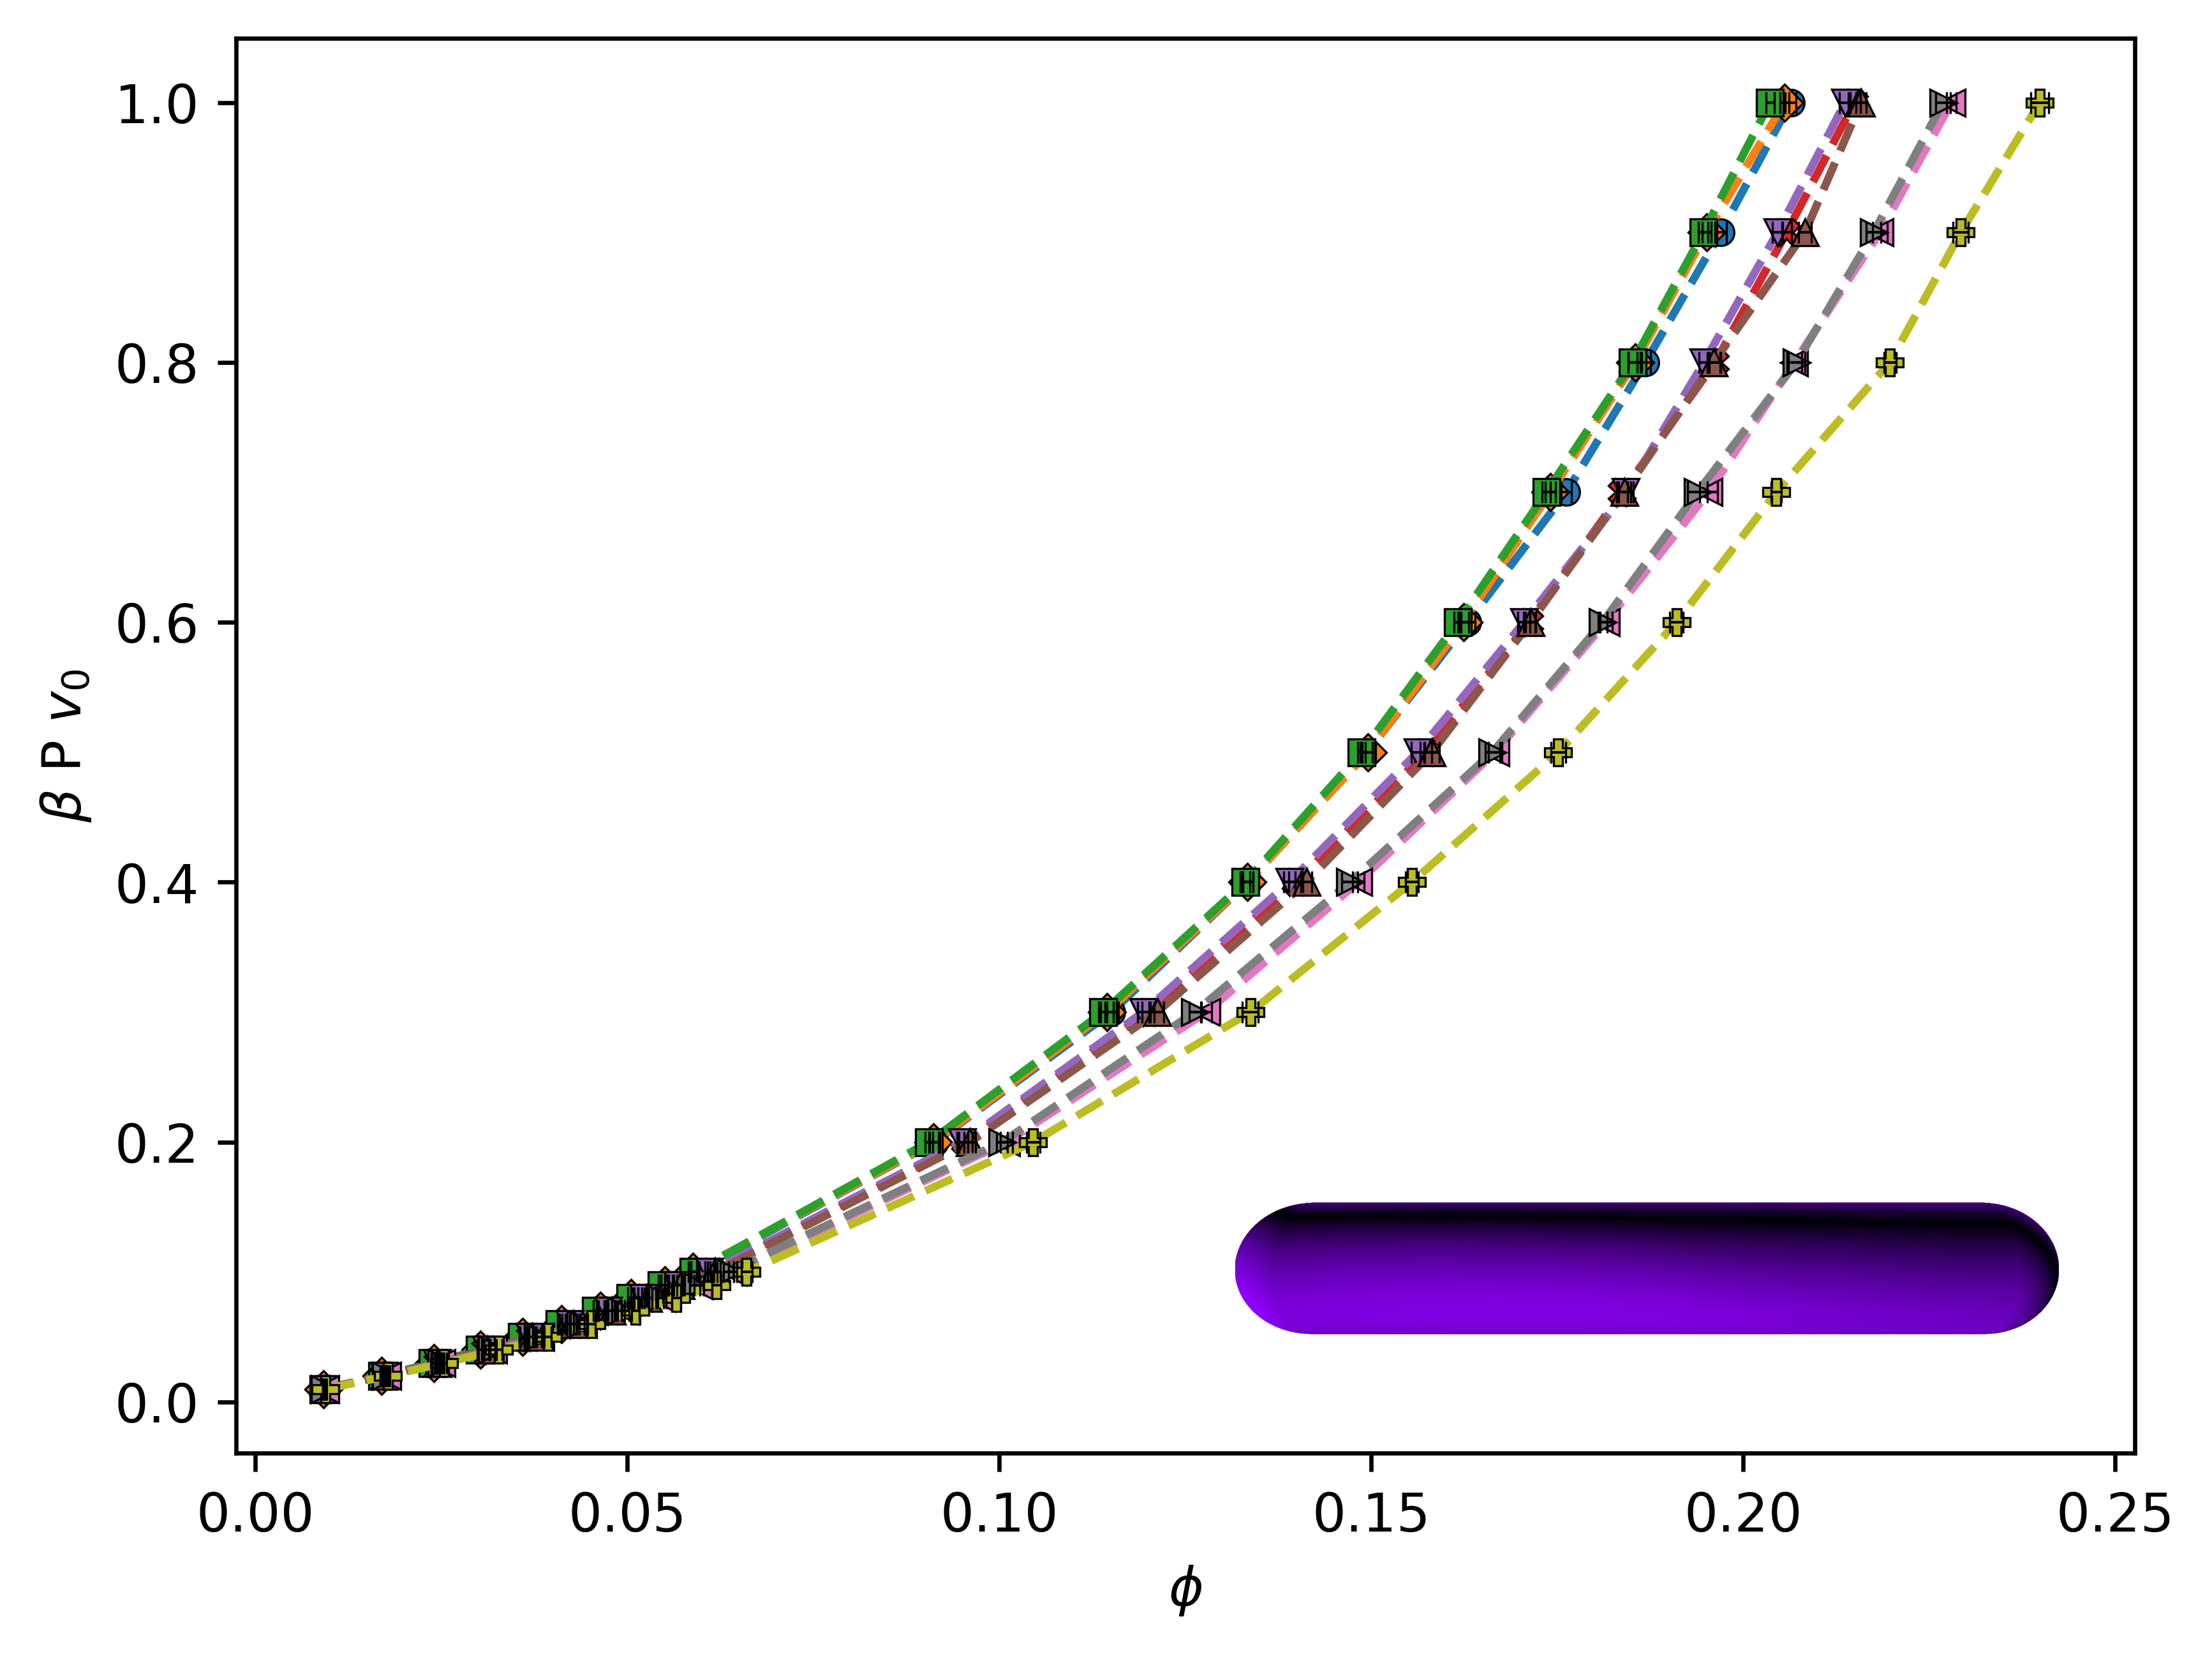
\includegraphics[width=0.45 \columnwidth]{Figures/EOS_A5.png}
	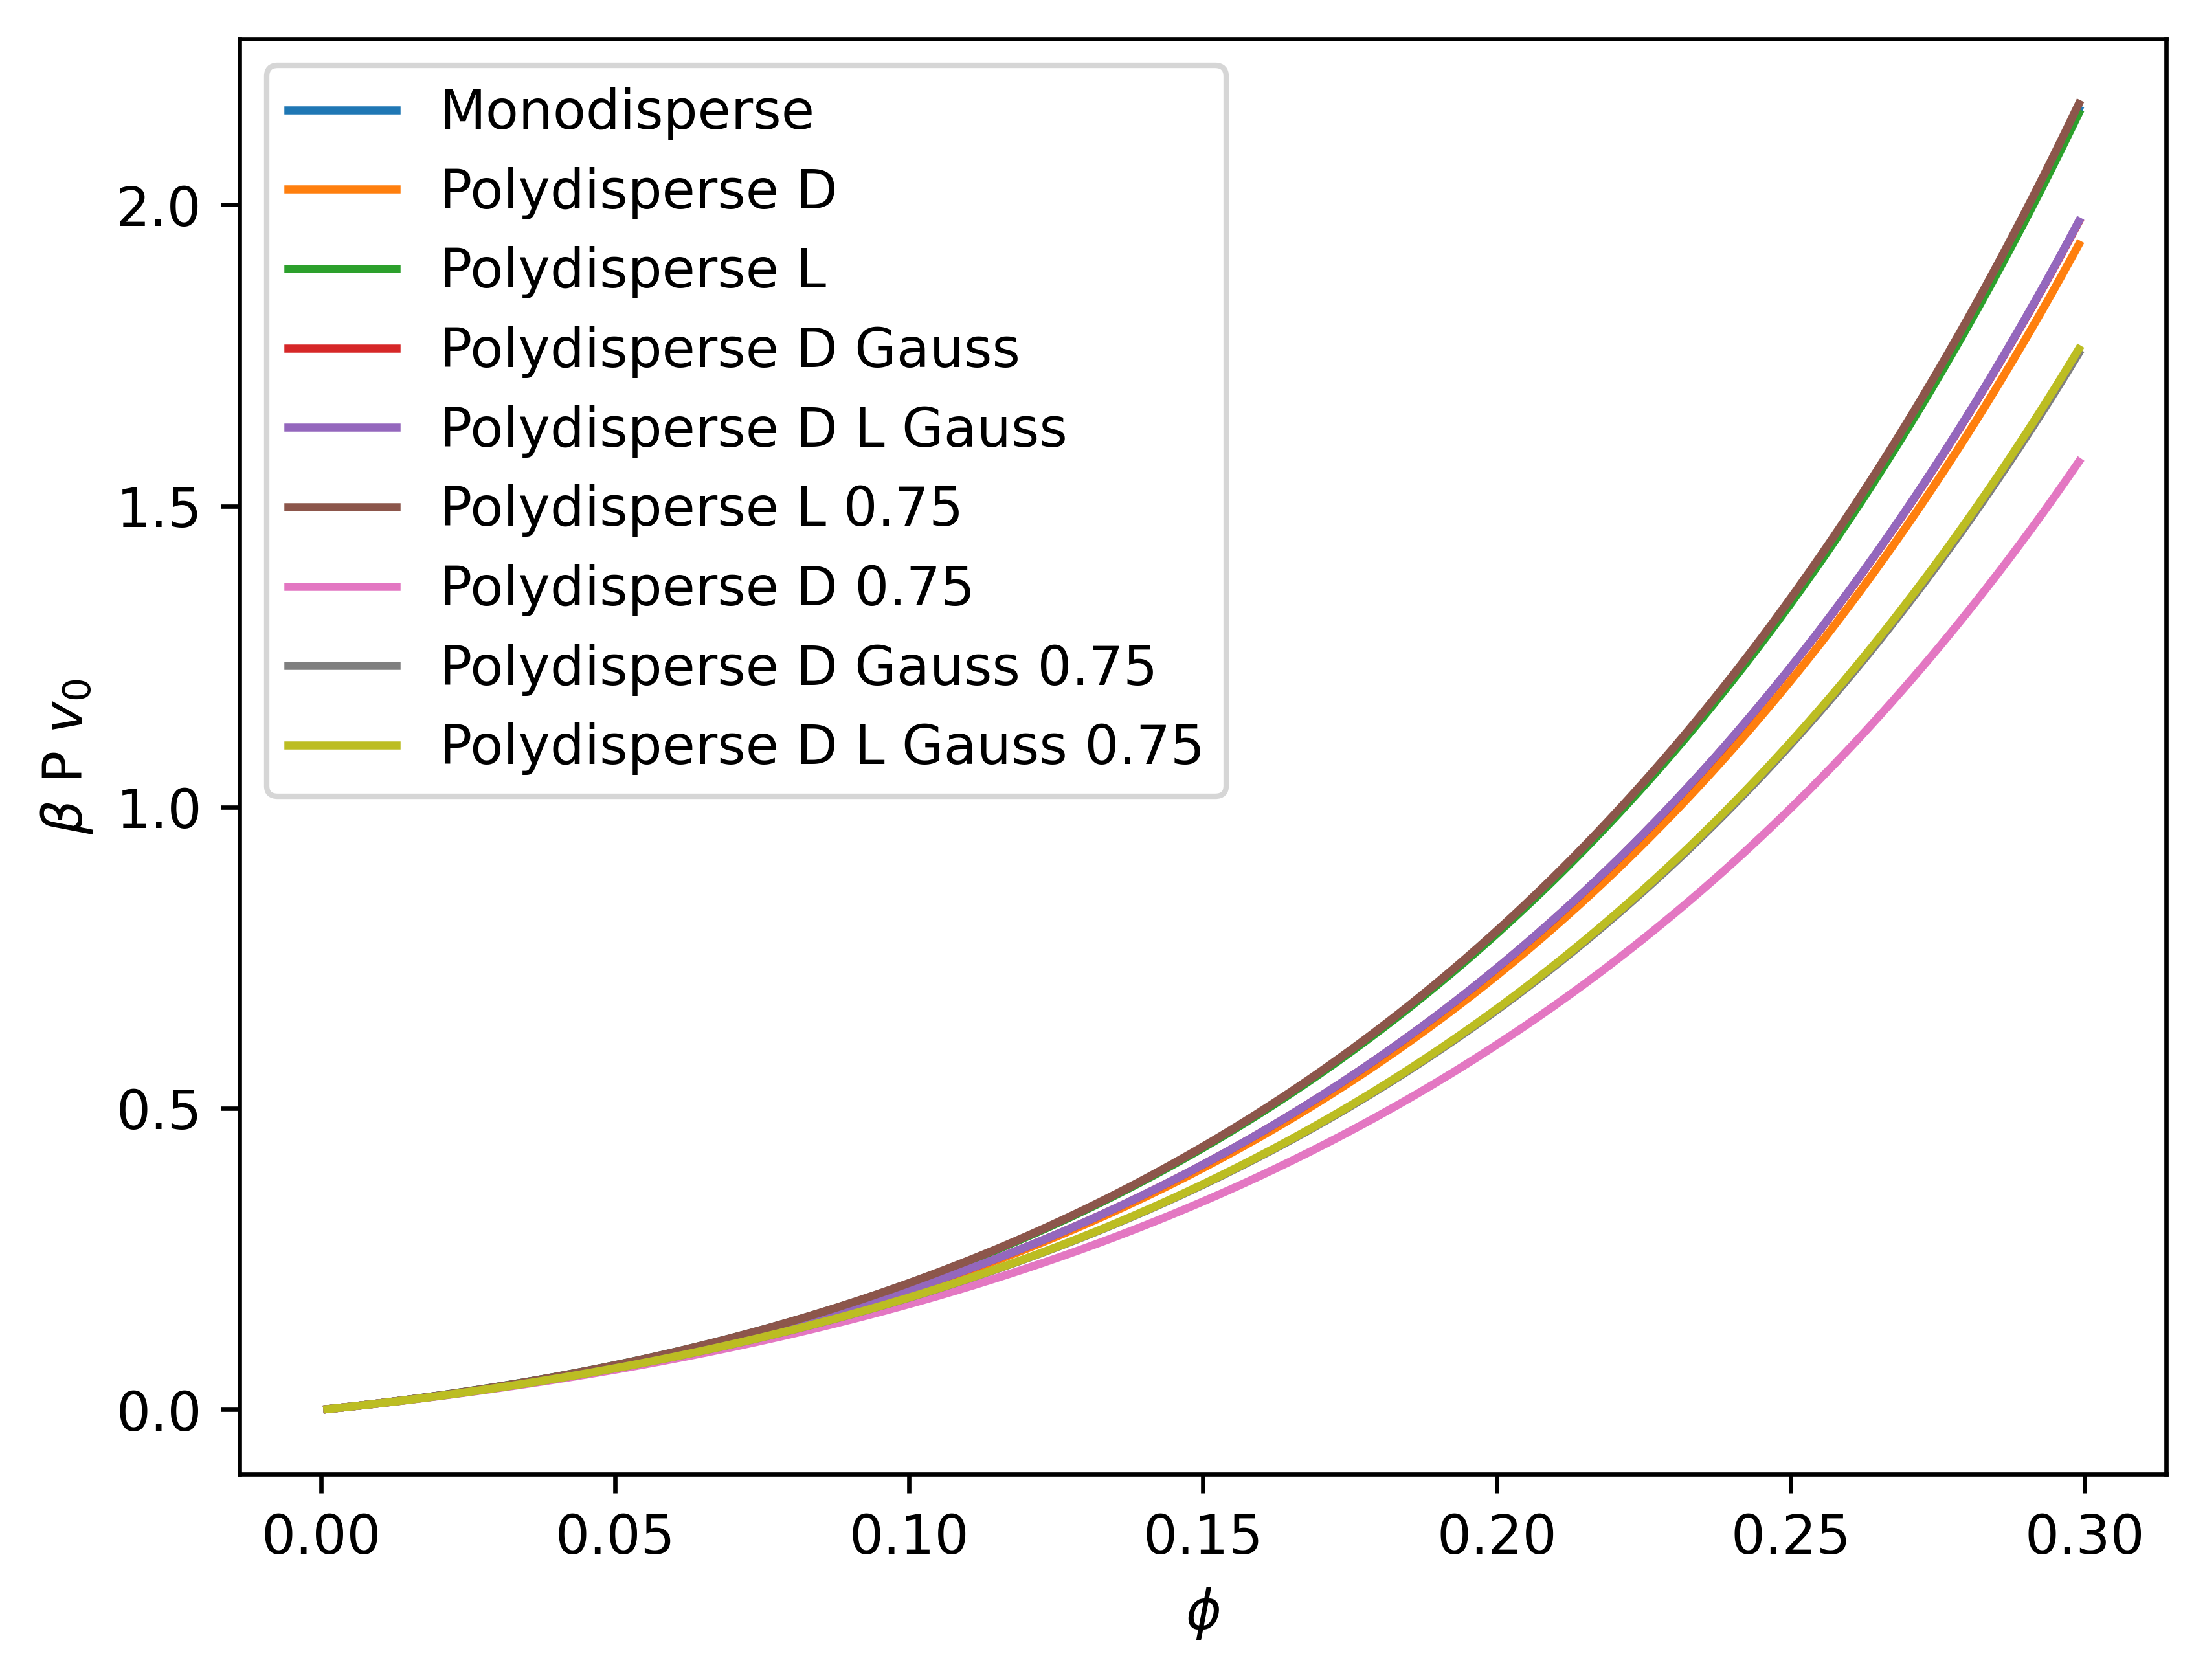
\includegraphics[width=0.45 \columnwidth]{Figures/EOS_Th_A5.png}
	\caption{Qualitative theory agreement. EOS of systems composed by particles with $A = 5$ obtained by the simulations (left) and via the Parson-Lee approximation (right). Monodisperse (circles), polydisperse L (diamonds), polydisperse L 75 \% (squares), Gauss polydisperse D (x symbols), Gauss polydisperse D and L (downward triangles), polydisperse D (upward triangles), Gauss polydisperse D 75 \% (leftward trinagles), Gauss polydisperse D and L 75 \% (rightward triangles), and polydisperse D 75 \% (plus symbols).}
	\label{fig:A5_comparison}
\end{figure}



\end{document}